\documentclass[review]{elsarticle}
\usepackage{lineno,hyperref}
% package added by zhixuan, not sure whether allowed by JCP or not!
\usepackage{amsmath}
\usepackage{float}

\modulolinenumbers[5]
\journal{Journal of Computational Physics}
%%%%%%%%%%%%%%%%%%%%%%%
%% Elsevier bibliography styles
%%%%%%%%%%%%%%%%%%%%%%%
%% To change the style, put a % in front of the second line of the current style and
%% remove the % from the second line of the style you would like to use.
%%%%%%%%%%%%%%%%%%%%%%%
%% Numbered
\bibliographystyle{model1-num-names}
%% Numbered without titles
%\bibliographystyle{model1a-num-names}
%% Harvard
%\bibliographystyle{model2-names.bst}\biboptions{authoryear}
%% Vancouver numbered
%\usepackage{numcompress}\bibliographystyle{model3-num-names}
%% Vancouver name/year
%\usepackage{numcompress}\bibliographystyle{model4-names}\biboptions{authoryear}
%% APA style
%\bibliographystyle{model5-names}\biboptions{authoryear}
%% AMA style
%\usepackage{numcompress}\bibliographystyle{model6-num-names}
%% `Elsevier LaTeX' style
%\bibliographystyle{elsarticle-num}
%%%%%%%%%%%%%%%%%%%%%%%
\begin{document}
\begin{frontmatter}
\title{Combining SPH with random choice method: a new scheme with adaptive artificial viscosity and shock capturing ability}
%\tnotetext[mytitlenote]{Can add  title note here}
%% Group authors per affiliation:
\author{Zhixuan Cao}
\author{Abani Patra \fnref{mycorrespondingauthor}}
\address{MAE Department,The State University of New York at Buffalo, Amherst, NY, 14260-4200, USA}
%\fntext[myfootnote]{Since 1880.}
%% or include affiliations in footnotes:
%\author[mymainaddress,mysecondaryaddress]%{Elsevier Inc}
%\ead[url]{www.elsevier.com}
%\author[mysecondaryaddress]{Global Customer Service\corref{mycorrespondingauthor}}
\cortext[mycorrespondingauthor]{Abani Patra}
\ead{abani@buffalo.edu}
%\address[mymainaddress]{1600 John F Kennedy Boulevard, Philadelphia}
%\address[mysecondaryaddress]{360 Park Avenue South, New York}
\begin{abstract}
Standard smoothed particle hydrodynamics (SPH) employs an artificial viscosity to properly capture hydrodynamical shock waves. In its original formulation, the artificial viscosity is large enough to 
%suppress structure in the velocity field on scales well above the nominal resolution limit, and to 
damp the generation of turbulence by fluid instabilities.
We present in this article a novel SPH scheme with adaptive artificial viscosity, in which the artificial viscosity is determined implicitly based on solution of a local Rieman Problem. Different from Godunov SPH (GSPH) method, which using solution of local Riemann problem at an imaginary interface, the new method randomly sample the solution of Riemann problem mimicking the random choice method (RCM). One dimensional shock tube tests demonstrate that this new method can capture shock waves while introducing less but sufficient artificial dissipation compared with classical SPH and GSPH. Combining of RCM with SPH also overcomes the inability of classical RCM method in solving multi-dimensional non-linear systems. Three dimensional time dependent Euler equations are solved for simulating an inject flow, demonstrating the ability of this new scheme for solving multi-dimensional non-linear systems. The tests also illustrate that the new method introduces much less dissipation for shearing flow than standard SPH and GSPH.
\end{abstract}
\begin{keyword}
Smoothed Particle Hydrodynamics (SPH), Random Choice Method, Hyperbolic PDEs, Rimemann Solver, Godunov method
\end{keyword}
\end{frontmatter}
\linenumbers
\section{Introduction}
Smoothed particle hydrodynamics (SPH) \citep{gingold1977smoothed,lucy1977numerical} is a meshfree particle method based on Lagrangian formulation, and has been widely applied to different areas in engineering and science. SPH has both advantages and disadvantages with respect to other numerical techniques. One main advantage is that it automatically adapts to following dynamic flows and arbitrary geometries. Another advantage is that it needs less programming effort to include more physics. In addition, SPH particles only interact with neighbouring particles, which avoids massive global communication in parallel implementation of SPH.

Historically, SPH has difficulty in capturing discontinuities, such as shocks or contact discontinuities. Inviscid description of fluids becomes invalid at shock fronts, where specific entropy of the fluids increases through the conversion of mechanical energy into internal. Most SPH codes have included an artificial viscosity term explicitly, both for stablizing the simulation and for handling shock discontinuities by dissipating local velocity differences and convert them into heat \citep{monaghan1983shock, monaghan1997sph, klapp2012strong}. Without knowing the minimum amount of dissipation for shock capturing, such methodology usually provides dissipation more than need and smears the discontinuity if the artificial viscosity coefficients are not tuned. The method of using constant artificial viscosity might also introduce spurious effects at region away from shocks, for instance, causing an unphysical damping of turbulent mixing (As shown, for example, by \citet{borgani2012hydrodynamic}) or spurious
shearing torques in rotating flows \citep{flebbe1994smoothed}. Selective application of artificial viscosity techniques, such as the time dependent viscosity \citep{morris1997switch, dolag2005turbulent} and shock-indicator-based viscosity \citep{cullen2010inviscid} have been tried for counteracting this. 
\citet{sigalotti2008adaptive} improved the standard SPH near sharp discontinuities adopting an adaptive density kernel estimation (ADKE) techniques. However, the parameters for ADKE have to be tuned to the problem at hand. Hence hard to implement for real implementations.

Besides adding dissipation explicitly, \citet{inutsuka2002reformulation} proposed an innovative approach to introduce dissipation implicitly by reformulating the SPH convolution integrals. Artificial viscosity is introduced implicitly by using iterative solution to a Riemann problem at an imaginary interface between an interacting particle pair. This method, named as Godunov SPH (GSPH), is attractive because it eliminates parameterization and hence user intervention associated with artificial viscosity coefficients. The GSPH method has been shown to be able to handle shock discontinuities \citep{inutsuka2002reformulation, cha2003implementations,iwasaki2011smoothed, puri2014approximate}, introduces less damping to turbulent mixing \citep{cha2010kelvin, borgani2012hydrodynamic} than standard SPH, and relieve pressure "blips" at the contact discontinuity \citep{borgani2012hydrodynamic}. However, the amount of dissipation introduced by GSPH is stll excessive than needs. When using a linear interpolation of the volume function, it has been shown \citep{borgani2012hydrodynamic} that the excess of diffusion, which manifests itself in the shock tube tests as a smooth transition at the rarefaction fan, is such to prevent the development of the Kelvin-Helmholtz (KH) instability.
The development of KH instability is also significantly affected by number of neighbouring particles for cubic interpolation of the volume function.

The random choice method (RCM) was introduced by \citet{glimm1965solutions} for the construction of solutions of systems of nonlinear hyperbolic conservation laws. \citet{chorin1976random} developed the RCM as a practical computational method for solutions to 1D Euler equations of gas dynamics. Chorin's work was followed by numerous researchers, with applications and further improvements \citep{sod1977numerical,concus1979numerical,colella1982glimm, freistuhler1992numerical}. In essence, the solution is advanced in time by a sequence of operations that includes the solution of Riemann problems and a stochastic sampling procedure. When applied to one dimensional time dependent Euler equations \citep{colella1982glimm}, diffusive errors from spatial averaging are completely eliminated and hence discontinuities, such as shocks or material interface, can be resolved as true discontinuities.
For unsteady flows in genuine two (or higher) space dimensions, however, such very desirable property of RCM do not seem to persist \citep{colella1982glimm}. Implementing of RCM within the framework of SPH only involves sampling of solutions of Riemann problem in one dimensional local coordinate system, even for multi-dimensional problems. Hence desirable property of RCM method in one dimension will be retained in higher dimensional implementations. 
%This need to be proven ---> But at least, if the good property of preserving true discontinuity is still valid in 1D shock tube problem, it should be preserved in multiple-dimensional implementations. Because in current framework of RSPH, no matter what is the dimension of the problem, the techniques is only implemented in a one-dimensional scenario. 

In this investigation, we introduce a new method, which will be refered to as RSPH in later paragraph, by combining RCM method with SPH. The RSPH inherits the attraction of classical RCM in handling complex wave interaction involving discontinuities such as shock waves and material interfaces. True discontinuity is resolved by RCM while most other methods would smear discontinuities.
%Need to prove by simulations
As RCM method is implemented within one dimensional local coordinate system, established for pair of interacting particles, hence does not involve multi-dimensional coordinates even for non-linear problems in a multi-dimensional space. Thereby, the attractive properties of RCM showing in one dimensional case is preserved in multi-dimensional implementations. the RSPH overcomes the fundamental shortcoming of RCM method, that is its inability in solving multi-dimensional (more than two dimentional) non-linear system .
Compared with classical SPH method, RSPH has the following advantages:
\begin{itemize}
\item RSPH is able to capture discontinuities with less smearing.
\item The RSPH is able to adaptively adjust equivalent artificial viscosity coefficients, assigning larger artificial viscosity coefficients around the shock and small artificial viscosity coefficients otherwhere.
\item RSPH is able to suppress pressure "wiggles? at the contact discontinuity, a common issue in classical SPH.
\end{itemize}
Compared with GSPH, which is also based on solution of local Riemann problem, RSPH introduces much less but sufficient dissipation than GSPH, especially in the region away from shocks. Such feature of RSPH is specially beneficial for simulating of scenarios involving turbulence mixing, for which excessive dissipation would suppress mixing.

The scheme of this paper is follows. We start with a brief review of standard SPH and GSPH in the second section. The RSPH is then explained in details in the third section followed by numerical test section, where both one dimensional (1D) and three dimensional (3D) inviscid Euler equations (see Eq. (\ref{eq:gov-cs-rho}) - (\ref{eq:gov-cs-e}) are solved by standard SPH, GSPH and RSPH. Limitations and potential application of RSPH are discussed in last section.
\begin{align}
\dfrac{\partial \rho}{\partial t} + \nabla \cdot \left(\rho \textbf{v} \right) = 0 \label{eq:gov-cs-rho} \\
\dfrac{\partial \rho \textbf{v}}{\partial t} + \nabla \cdot \left(\rho \textbf{v} \textbf{v} + p\textbf{I}\right) = 0 \label{eq:gov-cs-v} \\
\dfrac{\partial \rho E}{\partial t} + \nabla \cdot \left[\left(\rho E + p \right)\textbf{v}\right] = 0 \label{eq:gov-cs-e}
\end{align}
where $\rho$ is the density, $\textbf{v}$ is the velocity, $\textbf{I}$ is a unit tensor.
$E = e + K $ is the total energy which is a summation of kinetic energy $K$ and internal energy $e$.
The system of equations is closed by equation of state (EOS) for idea gas.
\begin{equation}
p = \left(\gamma - 1\right)\rho e \label{eq:EOS}
\end{equation}
with $\gamma=1.4$.
For SPH, governing equations in Lagrange form are needed. By deducting kinetic energy from energy equation, subtracting mass conservation from momentum equation, combining transient term and advection term into material derivative (for any function $A$, material derivative is defined as $\frac{D A}{Dt} = \frac{\partial A}{\partial t} + \textbf{v} \cdot \nabla A$) term, the governing equations are put into the final form. 
\begin{align}
\dfrac{D \rho}{D t} + \rho \nabla \cdot \textbf{v} = 0 \label{eq:gov-nc-rho}\\
\dfrac{D \textbf{v}}{D t} + \dfrac{\nabla P}{\rho} =0 \label{eq:gov-nc-v}\\
\dfrac{D e}{D t} + \dfrac{P \nabla \cdot \textbf{v}}{\rho} = 0 \label{eq:gov-nc-e}
\end{align}
%\cutet{puri2014comparison} propose an addition of an artificial heating term to the GSPH scheme to eliminate unphysical spikes in the thermal energy at the contact discontinuity.  --> It is worthwhile to check whether RSPH is able to avoid this phenomena without using his techniques.
%Another issue of RCM: the very desirable properties of RCM: no diffusive errors from spatial averaging do not seem to persist for flows in two space dimensions. For two dimensional steady supersonic flow, one of the space variables can be treated as a time-like one and ReM can be applied in a way similar to that for one-dimensional unsteady flow.
%--Then what about RSPH?
\section{Standard SPH and GSPH method}
The RSPH method is proposed based on standard SPH and GSPH. In addition, these three methods are compared in the numerical tests section. We present here a breif review on standard SPH and GSPH.
\subsection{Standard SPH method}
In SPH, the domain is discretized by a set of particles or discretization points and the position of each particle is updated at every time step based on the motion computed. Approximation of all field variables (velocity, density and pressure, ect.) is obtained by interpolation based on discretization points. The physical laws (such as conservation laws of mass, momentum and energy) written in the form of PDEs (partial differential equations) or ODEs (ordinary differential equations) need to be transformed into the Lagrangian particle formalism of SPH. Using a kernel function that provides the weighted estimation of the field variables at any point, the integral equations are estimated as sums over particles in a compact subdomain defined by the support of the kernel function associated with the discretization points. Thus, field variables associated to the particle are updated based on its neighbors. Each kernel function has a compact support determined by smoothing length of each particle. Various tricks can be used to conserve linear and angular momentum and thermal energy \citep{monaghan1992smoothed}. Special treatments are also needed for second order derivative terms \citep{monaghan2005smoothed}. We only refer here to one of these possible discretizations of compressible Euler equations, while we refer to \citet{ monaghan2005smoothed, liu2010smoothed, price2012smoothed} for complete formal derivation.
\begin{align}
<\rho_a> = \sum_b m_b w_{ab} \left(h\right) \label{eq:ns-sph-d} \\
\left\langle\dfrac{d \textbf{v}_a}{d t}\right\rangle = -\sum_b m_b \left(\dfrac{p_b}{\rho_b^2} + \dfrac{p_a}{\rho_a^2} + \Pi_{ab}\right) \nabla_a w_{a b}\left(h\right) \label{eq:ns-sph-v} \\
\left\langle\dfrac{d e_a}{d t}\right\rangle=
 0.5\sum_b m_b \textbf{v}_{a b}\left(\dfrac{p_b}{\rho_b^2} + \dfrac{p_a}{\rho_a^2} + \Pi_{ab}\right) \cdot \nabla_a w_{a b}\left(h\right) \label{eq:ns-sph-e}
\end{align}
where, $a$ is the SPH particle index, $\textbf{v}_{a b} = \textbf{v}_a - \textbf{v}_b$. $\Pi$ is an artificial viscosity term.
One of commonly used models of artificial viscosity \citep{monaghan1983shock} is:
\begin{equation}
\Pi_{ab}=- \frac{\nu}{\bar{\rho}_{ab}} \dfrac{ \textbf{v}_{ab} \cdot \textbf{x}_{ab}}{\textbf{x}_{ab}^2 + \left(\eta h\right)^2}
\label{eq:art-vis-original}
\end{equation}
The coefficient $\nu$ is defined as:
\begin{equation}
\nu = \alpha \bar{h}_{ab} \bar{c}_{ab}
\end{equation}
where 
\begin{align}
\bar{c}_{ab} = \dfrac{c_a + c_b}{2} \\
\bar{\rho}_{ab} = \dfrac{\rho_a + \rho_b}{2} \\
\textbf{v}_{ab}=\textbf{v}_a-\textbf{v}_b \\
\textbf{x}_{ab}=\textbf{x}_a-\textbf{x}_b
\end{align}
The artificial viscosity term $\Pi_{ab}$ is a Galilean invariant and vanishes for rigid rotation. It produces a repulsive force between two particles when they are approaching each other and an attractive force when they are receding from each other.
An extra term was added to $\nu$ considering aspects of the dissipative term in shock solutions based on Riemann solvers and lead to a new formulation of artificial viscosity. We adopt this new formulation in our simulation:
\begin{equation}
\Pi_{ab}^{\beta} = 
\begin{cases} 
      \dfrac{- \alpha \mu_{ab} \bar{c}_{ab} + \beta \mu_{ab}^2} {\bar{\rho}_{ab}} & \textbf{v}_{ab} \cdot \textbf{x}_{ab} < 0\\
      0 & \textbf{v}_{ab} \cdot \textbf{x}_{ab} > 0
\end{cases}
\label{eq:art-vis-shock}
\end{equation}
where
\begin{equation}
\mu_{ab} = \dfrac{h \textbf{v}_{ab} \cdot \textbf{x}_{ab}}{\textbf{x}_{ab}^2 + \left(\eta h\right)^2} 
\end{equation}
%$\alpha$ and $\beta$ are two parameters that are free to be adjusted for each case. 
$\alpha$ and $\beta$ are two parameters that can be adjusted for different cases.
$\alpha = 1$ and $\beta = 2$ are recommended by Monaghan for best results and mostly adopted. In the numerical test section, these two parameters are varied to show the effect of them. $\eta$ is usually taken as 0.1 to prevent singularities.

In Eq. (\ref{eq:ns-sph-d}) - Eq. (\ref{eq:ns-sph-e}), $w_{a b}\left(h\right)$ is weighting function and is a concise form of $w\left(\textbf{x}_a - \textbf{x}_b, h\right)$. From here on, we will use this concise form.
There is a wide variety of possible weighting functions, such as spline functions (with different orders) and Gaussian functions. We are adopting a truncated Gaussian function as the weighting function for standard SPH, GSPH and RSPH.
\begin{equation}
w\left(\textbf{x} - \textbf{x} \prime \right) = 
\begin{cases} 
      \dfrac{1}{\left(h \sqrt{\pi}\right)^d} exp \left[- \left(\dfrac{\textbf{x} - \textbf{x} \prime}{h} \right)^2 \right] &  \vert \textbf{x} - \textbf{x} \prime \vert \leq 3h\\
      0 & \text{Otherwise}
\end{cases}
\label{eq:SPH-kernel}
\end{equation}
where $d$ is number of dimensions.
The derivative of the weighting function is:
\begin{equation}
\nabla w\left(\textbf{x} - \textbf{x} \prime \right) = 
\begin{cases} 
      -2\left(\dfrac{\textbf{x} - \textbf{x} \prime}{h}\right) \dfrac{1}{\left(h \sqrt{\pi}\right)^d} exp \left[- \left(\dfrac{\textbf{x} - \textbf{x} \prime}{h}\right)^2 \right] &  \vert \textbf{x} - \textbf{x} \prime \vert \leq 3h\\
      0 & \text{Otherwise}
\end{cases}
\label{eq:SPH-kernel-gradient}
\end{equation}

As a Lagrangian method, particle position is also updated at every time step.
\begin{equation}
\left\langle\dfrac{d \textbf{x}_a}{dt}\right\rangle = \textbf{v}_a \label{eq:SPH-update-pos}
\end{equation}

\subsection{GSPH method}
Here we present essential formulations for solving Euler equations with GSPH. The density field is updated in the same way as updating of density in SPH, according to Eq. (\ref{eq:ns-sph-d}). Updating of velocity and internal energy in GSPH is different from these in SPH. 
Derivation of discretized momentum and energy equation in first GSPH paper \citep{inutsuka2002reformulation} is based on the following discreted consistency identities: 
\begin{equation}
1=\sum_{b} \frac{m_{b}}{\rho(\textbf{x})}w(\textbf{x} - \textbf{x}_{b}, h)
\label{eq:GSPH-basic1}
\end{equation}
\begin{equation}
0=\sum_{b} m_{b} \nabla \frac{w(\textbf{x} - \textbf{x}_{b}, h)}{\rho(\textbf{x})}
\label{eq:GSPH-basic2}
\end{equation}
Lengthy algebraic manupulations \citep{inutsuka2002reformulation,iwasaki2011smoothed, } lead to the discretized momentum and energy equations:
\begin{equation}
\ddot{\textbf{x}}_{a} = <\dfrac{d \textbf{v}_{a}}{dt}>= -\sum_{b} m_{b} p_{a b}^{\ast} \left[\frac{1}{\rho_{a}^2} \nabla w_{a b}(h_{a}) + \frac{1}{\rho_{b}^2} \nabla w_{a b}(h_{b}) \right]
\label{eq:gov-gsph-v-simple-form}
\end{equation}
\begin{equation}
<\dfrac{d e_{a}}{dt}>= - \sum_{b} m_{b} p_{a b}^{\ast} [\textbf{v}_{a b}^{\ast} - \dot{\textbf{x}}_{a}^{\ast}] \left[\frac{1}{\rho_{a}^2} \nabla w_{a b}(h_{a}) + \frac{1}{\rho_{b}^2} \nabla w_{a b}(h_{b}) \right]
\label{eq:gov-gsph-e-simple-form}
\end{equation}
Where, $p_{a b}^{\ast}$ and $\textbf{v}_{a b}^{\ast}$ is obtained by solving a 1D Riemann problem constructed based on state of particle $a$ and particle $b$.
$\dot{\textbf{x}}_{a}^{\ast}$ is time centered velocity of particle $a$:
\begin{equation}
\dot{\textbf{x}}_{a}^{\ast} = <\textbf{v}_{a}> + \frac{\Delta t}{2} \ddot{\textbf{x}}_{a}
\end{equation}
The difference between this formulation and classical SPH formulations come from two sources: 
\begin{itemize}
\item the averaged (in certain sense) pressure and the effect of artificial viscosity is replaced by  $p^{\ast}$, obtained based on a local Riemann solver.
\item A time centered velocity is used, which satisfies the following identities approximately. 
\begin{equation}
\left( \textbf{v}_{a b}^{\ast} - \dot{\textbf{x}}_{a}^{\ast} \right) \approx -0.5 \textbf{v}_{a b}
\label{eq:SPH-GSPH-difference2}
\end{equation}
Where $\textbf{v}_{a b}$ is defined as $\textbf{v}_a - \textbf{v}_b$.
\end{itemize}
Actually, Godunov's idea of using Riemann solver can be combined with other SPH discretization formulations \citep{cha2003implementations}.

The constructing of Riemann problem, Riemann solvers and projection of picked solution back to global coordinate system are similar in both GSPH and RSPH, which will be described in detail in the next section. The way how solutions of Riemann problems are used is different in GSPH and RSPH. In GSPH, solution of Riemann problem at an imaginary interface is picked up, either based on interpolation of specific volume \citep{inutsuka2002reformulation} or simply assuming a middle points interface \citep{cha2003implementations}. RSPH takes solution of Riemann problem based on random sampling.

\section{RSPH method}
For mesh based method, there is a great deal of commonality between Godunov's method and RCM. Both of them utilize the solution of a local Riemann problem. While Gounov's method take the intergratal average, the RCM pick up a single state contained in the local solutions "randomly". The random selection procedure is carried out by employing a sequence of random numbers. The Godunov's SPH method (GSPH) actually does not take the intergratal average, a single state of a local Riemann solution at a imaginary inteface is picked up and used to upgrade physical quantities through discretized governing equations of SPH summation. So the difference between RSPH and GSPH is how to pick up the single state. RSPH pick up the single state randomly while GSPH chooses the single state at an imaginary interface.
Since the only difference between Godunov's method and RCM is how the solution of local Riemann problem is utilised, we can use exact the same discretization in RSPH as in GSPH. In addition, the construction of 1D Riemann problem for RSPH is the same as piecewise constant contruction of Riemann problem for GSPH. 
It is a commom practice in real implementation of Godunov's method to use approximate non-iterative Riemann solvers. This strategy is also adopted for RSPH. The one that we choose to use is a HLLC type of Riemann solver \citep{toro1994restoration}, in which the contact wave is also solved.

\subsection{Constructing of 1D Riemann problem}
Even for a 2D and 3D problems, only a 1D Riemann problem need to be solved to obtain  $p_{a b}^{\ast}$ and $\textbf{v}_{a b}^{\ast}$. Hence, a 1D Riemann problem need to be construted. Constructing of 1D Riemann problem starts from establishing of a local coordinate systems ($q$). The origin is at the middle-point of the line segment joining two particles with the unit vector along the line defined as: 
\begin{equation}
\hat{r}_{a b}= \frac{\textbf{v}_{a} - \textbf{v}_{ b}}{|\textbf{x}_{a} - \textbf{x}_{ b}|}
\end{equation}
Then project velocity onto the local coordinate system.
\begin{equation}
u_{a}= \textbf{v}_{a} \cdot \hat{r}_{a b}
\end{equation}
\begin{equation}
u_{b}= \textbf{v}_{b} \cdot \hat{r}_{a b}
\end{equation}
In Godunov's SPH method, the construction of Riemann problem is divided into two sub-steps: projection and construction. 
Different from Godunov's method, which assumes piecewise constant distribution of the data (for higher order method like MUSCL and PPM, they use higher order polynomial approximation.), RCM method assumes that the given data at the center of cell is constant throughout the respective cell. The same idea can be easily (and naturally) applied in RSPH, as there is actually no "cell interface" in SPH method.
In this case, no additional steps for constructing a Riemann problem is needed. The Riemann problem is defined directly based on data on particles. There is no need to calculate and project first order derivative of $\rho$, $u$ and $p$ any more. The computation associated with calculation of gradient and projection of gradient is avoid in RSPH. So it is supposed to be more computationally efficient than GSPH.
Solving the 1D Riemann problem with initial right and left states that the same as those on the paired particles leads to a solution of the local system. Then random sample these solutions to pick up a state and assign its corresponding state to $p^{\ast}$ and $u^{\ast}$. 
Assume the solution between of a pair of particles ($a$ and $b$) to be $\textbf{W} (q) \forall q \in [q_a, q_b]$ (note, we use $\textbf{W}$ to represent the primitive variable vector $[\rho, u, p]^T$ and $\textbf{U}$ for conservative variable vector  $[\rho, \rho u, \rho E]^T$). The star values would depends on the random number $\epsilon$.
\begin{equation}
p^{\ast} = p \left(\epsilon \left( q_a - q_b \right) \right)
\label{eq:RSPH-Random-Pick-p}
\end{equation}
\begin{equation}
u^{\ast} = u \left(\epsilon \left( q_a - q_b \right) \right)
\label{eq:RSPH-Random-Pick-u}
\end{equation}
A short comments regarding the difference between application of RCM method in SPH and its application in finite volume method. In finite volume method, the superposition of solutions of Riemann problems defined on boundaries is taken as local solution within the cell and the sampled single state is assigned to the cell center. In RSPH, only one Riemann problem is defined between two particles and the sampled single state (the $p^{\ast}$ and $u^{\ast}$) is used in momentum and energy updating.
Then it needs to project $u^{\ast}$ back to the 3D coordinate system to obtain $\textbf{v}^{\ast}$. One of such back-project approximations is:
\begin{equation}
\textbf{v}^{\ast}_{a b}=u^{\ast}_{a b} \hat{\textbf{r}}_{a b} + \left [\frac{\textbf{v}_{a} + \textbf{v}_{b}}{2} - \frac{u_L + u_R}{2} \hat{\textbf{r}}_{a b}\right]
\label{eq:RP-project-to-3d-arithmetic}
\end{equation}
In Eq. (\ref{eq:RP-project-to-3d-arithmetic}), the arithmetic average of shear velocity is taken as the shear velocity in the star region. Alternative approximation might be distance weighted average or Roe average (weighted by square root of density). If $q_{a b}^{\ast}$ is assumed to be zero, then distance weighted average will degenerate to the arithmetic average.
%Eigenstructure analysis shows that there are two additional contact discontinuity waves for 3D Euler equations. They are associated to two shear velocity components. Different from $u$ and $p$, the shear velocity is not constant in the star region. Using the average of left and right shear velocity as an approximate of shear velocity in the star region might be a poor approximation.
We have to mention that it is strange in GSPH to assume an imaginary interface, which we never need in RSPH. And that's one of the reasons why we like RSPH more.
\subsection{Approximate Riemann solvers}
The stared variable $p^{\ast}$ and $u^{\ast}$ represent the interpolated pressure and velocity at some point (the "interface" in GSPH, a random poit in RSPH) along the line joining the pairs of two particles. They do not have to be obtained by solving a Riemann problem. However, $p^{\ast}$ and $u^{\ast}$ obtained by solving a Riemann problem provides necessary and sufficient dissipation needed to stablize the shceme. 
%From numerical analysis point of view, numerical dissipation is necessary for numerical stability. From physics point of view, viscosity is a necesssary condition for shock formation. But Euler equations are based on assumption of invisd, which means Euler equation themselves are not capable to represent shock formation correctly. Adding of artificial viscosity helps fix the "birth defect" of Euler equations. 

The exact Riemann solver even though more accurate and robust, requires an interative root finding, and hence is computational inefficient. For governing equations other than well studied ones , such as Euler equation, no exact Riemann solver available. Non-iterative approximate Riemann solvers can relieve these drawbacks of exact Riemann solvers. Among the available Reimann solvers \citep{rider1994review, luo2004computation, puri2014approximate}, we adopted the Harten, Lax and van Keer shceme with contact (HLLC).
The HLLC solver is a 3-wave approximate Riemann solver proposed by \citet{toro1994restoration}. In this work, we adopt the formulation of the HLLC solver proposed by \citet{luo2004computation} for multi-material, underwater explosions in their ALE scheme. This Riemann solver has the properties of being positivity preserving for scalar quantities, entropy satisfying and to exact preserve isolated contacts.

The expression for itermediate pressure and velocity can be written as \citep{puri2014approximate}:
\begin{equation}
p^{\ast} =  \begin{cases} 
      p_L & if \  S_L > 0 \\
      \frac{S_M}{S_L - S_M}\left [ (S_L - \hat{u}_L) M_L + (\hat{p}- p_L) \right] + \hat{p} & if \  S_L \leq 0 \leq S_M \\
      \frac{S_M}{S_R - S_M}\left [ (S_R - \hat{u}_R) M_R + (\hat{p}- p_R) \right] + \hat{p} & if \  S_M \leq 0 \leq S_R\\
      p_R & if \  S_R < 0
\end{cases}
\label{eq:RP_solver_HLLC_u}
\end{equation}
\begin{equation}
(pu)^{\ast} =  \begin{cases} 
      p_L u_L& if \  S_L > 0 \\
      \frac{S_M}{S_L - S_M}\left [ (S_L - \hat{u}_L) E_L + (\hat{p} S_M - p_L \hat{u}_L) \right] + (S_M - \hat{u}_{LR}) \hat{p} & if \  S_L \leq 0 \leq S_M \\
      \frac{S_M}{S_R - S_M}\left [ (S_R - \hat{u}_R) E_R + (\hat{p} S_M- p_R \hat{u}_R) \right] + (S_M + \hat{u}_{LR}) \hat{p} & if \ S_M \leq 0 \leq S_R\\
      p_R u_R & if \  S_R < 0
\end{cases}
\label{eq:RP_solver_HLLC_pu}
\end{equation}
where $\hat{u}_LR$ is the interface velocity and is taken as the Roe-averaged velocity on either side of the interface. The quantities of $\hat{u}_R$ and $\hat{u}_L$ are velocities relative to the interface velocity.
\begin{equation}
\hat{p}= \rho_L (\hat{u}_L - S_L) (\hat{u}_L - S_M) + p_L
\end{equation}
One formulation to approximate the signal speeds $S_M$, $S_L$ and $S_R$ is given by Eq. (\ref{eq:RP-solver-HLLC-SM}) to (\ref{eq:RP-solver-HLLC-SR}) (WaveEva0).
\begin{eqnarray}
S_M= \frac{\rho_R \hat{u}_R (S_R - \hat{u}_R) - \rho_L \hat{u}_L (S_L - \hat{u}_L) + p_L - p_R}{\rho_R (S_R - \hat{u}_R) - \rho_L (S_L - \hat{u}_L)} \label{eq:RP-solver-HLLC-SM} \\
S_L = min (\hat{u}_L - c_L, -c_{LR}) \label{eq:RP-solver-HLLC-SL} \\
S_R = max (\hat{u}_R - c_R, c_{LR}) \label{eq:RP-solver-HLLC-SR}
\end{eqnarray}
where $c_{LR}$ is the relevant Roe averaged sound speed.

%There are other different ways to estimate the singal speeds \citep{davis1988simplified, einfeldt1991godunov, batten1997average, toro2013riemann}.
%\citet{davis1988simplified} proposed a simplified formulation (WaveEva2):
%\begin{eqnarray}
%S_L = min (\hat{u}_L - c_L, u_R-c_{R}) \label{eq:RP-solver-HLLC-SL-David} \\
%S_R = max (\hat{u}_R - c_R, u_L-c_{L}) \label{eq:RP-solver-HLLC-SR-David}
%\end{eqnarray}
%The speed of the middle wave is still esitmated according to Eq. (\ref{eq:RP-solver-HLLC-SM}).
%\citet{toro2013riemann} suggests to adopt the pressure-based approximate-state Riemann solver (WaveEva3).
%\begin{eqnarray}
%S_L = min (\hat{u}_L - c_L, q_L c_{L}) \label{eq:RP-solver-HLLC-SL-Toro} \\
%S_R = max (\hat{u}_R - c_R, q_R c_{R}) \label{eq:RP-solver-HLLC-SR-Toro}
%\end{eqnarray}
%where 
%\begin{equation}
%q_K=  \begin{cases} 
%      1, & if \ p_{\ast} \leq p_K \\
%      \left[ 1 + \frac{1+\gamma}{2 \gamma} \left( \frac{p_{\ast}}{p_k} - 1 \right) \right] ^{0.5}, & p_{\ast} > p_K
%      \end{cases}
%\end{equation}
%for $K=L, R$, and 
%\begin{equation}
%p_{\ast} = max (0, p_{pvrs})
%\end{equation}
%\begin{equation}
%p_{pvrs}=\frac{p_L + p_R}{2} + \frac{u_L - u_R}{8}(\rho_L + \rho_R)(c_L + c_R)
%\end{equation}
%The speed of the middle wave is still esitmated according to Eq. (\ref{eq:RP-solver-HLLC-SM}). 

\subsection{Binary Van Der Corput pseudo-random numbers}
The random number $\epsilon$ is used to determine which single state ($p^{\ast}$ and $\textbf{v}^{\ast}$) of the solution of Riemann problem should be used in Eq. (\ref{eq:gov-gsph-v-simple-form}) and (\ref{eq:gov-gsph-e-simple-form}). The quantity of the computed RCM solution depends crucially on the random number $\{\epsilon ^n\}$.

A general Van Der Corupt pseudo-random number sequence depends on two parameters $x_1$ and $x_2$ with $x_1 > x_2 > 0$ both interger and relatively prime. The sequence is formally defined as \citep{hammersley2013monte}:
\begin{equation}
\epsilon ^n = \sum_{i=0}^{s} H_i x_1^{-(i+1)}
\label{eq:Van-Der-Corput-pseudo-random-num}
\end{equation}
where
\begin{equation}
H_i = x_2 a_i(mod x_1)
\label{eq:Van-Der-Corput-pseudo-random-num-Hi}
\end{equation} 
\begin{equation}
n = \sum_{i=0}^{s} a_i x_1^i
\label{eq:Van-Der-Corput-pseudo-random-num-n}
\end{equation} 
Equation (\ref{eq:Van-Der-Corput-pseudo-random-num-n}) gives the binary expansion of n when we take $x_1$ as $2$. For example,
\begin{equation}
5=1 \times 2^0 + 0 \times 2^1 + 1 \times 2^2
\end{equation}
and m=2. 

The next stage is to find the coefficient $H_i$ according to Eq. (\ref{eq:Van-Der-Corput-pseudo-random-num-Hi}). If we take $x_2 = 1$, for which case, $H_i = a_i, \ \forall i$. Having $H_i$, $x_1$ and $m$ ready, the random number $\epsilon ^n $ can be easily obtained according to Eq. (\ref{eq:Van-Der-Corput-pseudo-random-num}).
We take $x_1=2$  and $x_2 =1$ in our application. Other combinations of $x_1$ and $x_2$ were also discussed by \citet{toro2013riemann}. A desirable statistical property of the sequence $\{\epsilon ^n\}$ is that $\{\epsilon ^n\}$ be uniformly distributed over $[0,1]$.
 
The arithmetic mean and the standard deviation of 200 binary Van Der Corput pseudo-random numbers are $0.49459$ and $0.28885$. The chi-square statistic (see \citet{toro2013riemann} for its calculation) $\chi_{sq}$ is $1.0000$. 
The binary Van Der Corput pseudo-random numbers can be generated offline to save computational time.

\subsection{Convergence}

\subsection{RSPH algorithm (the PESB algorithm)}
The Godunov's method is summarized as a REA (reconstruct, evolve, average) algorithm. Here we summarize the RSPH algorithm as a PESB (project, evolve, smaple, back-project) algorithm. 
\begin{itemize}
\item For any two pair of particles, establish a local coordinate system whose axis joints these two particles then project the primitive variables vector onto the local coordinate system.
\item Evolve the hyperbolic equation exactly or approximately with the projected data to obtain a solution between these two particles.
\item Sample these solutions between the particles pair to pick up a state and assign it to $p^{\ast}$ and $u^{\ast}$
\item Project $p^{\ast}$ and $u^{\ast}$ from local coordinate system back to the global coordinate system obtaining $p^{\ast}$ and $\textbf{v}^{\ast}$.
\end{itemize}

\section{Numerical tests}
\subsection{1D shock tube tests input parameters}
One dimentional shock tube tests are conducted to compare standard SPH, GSPH and RSPH. Comprehensive shock tube tests are also carried out to check the capacity of RSPH for different situations. In addition, order of accuracy is investigated based on 1D shock tube prolem. Details of all tests can be found in Table \ref{tab:1D-shock-input_parameters}.
\begin{table}[htp]
\centering
      \caption{Overview of 1D shock tube tests}		
	  \begin{tabular}{lrrrrrrrrrr}
	    \hline
	          & $\rho_L$ & $p_L$ &$v_L$ & $\rho_R$ & $p_R$ &$v_R$ & $\Delta x$ & $[x_L, x_R]$ & $t_f$\\
	    \hline
	    Test 1 & $1.0$ & $1.0$ &$0$ & $0.25$ & $0.1795$ &$0$ & $0.00075$  & $[-0.4, 0.4]$ & $0.17$\\
	    	Test 2 & $1.0$ & $1.0$ &$0$ & $0.5$ & $0.2$ &$0$ & $0.0015$  & $[-0.4, 0.4]$ & $0.2$\\
	    	Test 3 & $2.0$ & $1.95$ &$1.0$ & $1.0$ & $1.95$ &$-1.0$  & $0.0015$  & $[-0.4, 0.4]$ & $0.13$\\
	    Test 4 & $1.0$ & $2.4$ &$8.0$ & $0.5$ & $0.4$ &$-0.25$ & $0.0015$  & $[-0.4, 0.4]$ & $0.05$\\
	    	Test 5 & $1.0$ & $-2.0$ &$0.4$ & $1.0$ & $0.4$ &$2.0$ & $0.003$  & $[-0.4, 0.4]$ & $0.18$\\
	    	Test 6 & $1.0$ & $0$ &$1000$ & $1.0$ & $0$ &$0.01$ & $0.003$  & $[-0.5, 0.5]$  & $0.01$\\
	    \hline
	  \end{tabular}
	  \label{tab:1D-shock-input_parameters}
\end{table}
where, subscript $L$ refers left side and $R$ for right side. $\Delta x$ is interval between two adjcent particles. $t_f$ is the time to terminate simulation and ploting the results. Equal particle mass is assigned to all particles. The x axis is normalized by time, that is $x/t_f$, in plots for shock tube tests resutls.

Test 1 consists of a left rarefaction, a right travelling contact and a right shock. Density increases at down wind of contact wave.
Test 2 also consists of a left rarefaction, a right travelling contact and a right shock. Density decreases at down wind of contact wave.
Test 3 is a double expansion test with different initial dnesity.
Test 4 is a double shock tests with different initial density on the right side and left side.
Test 5 and Test 6 are two extreme cases. Test 5 is a cavity flow while test 6 is a strong blast flow.

\subsection{Comparison of RSPH with standard SPH and GSPH}

\begin{figure}[H]
    \centering
    \begin{minipage}{.495\textwidth}
        \centering
        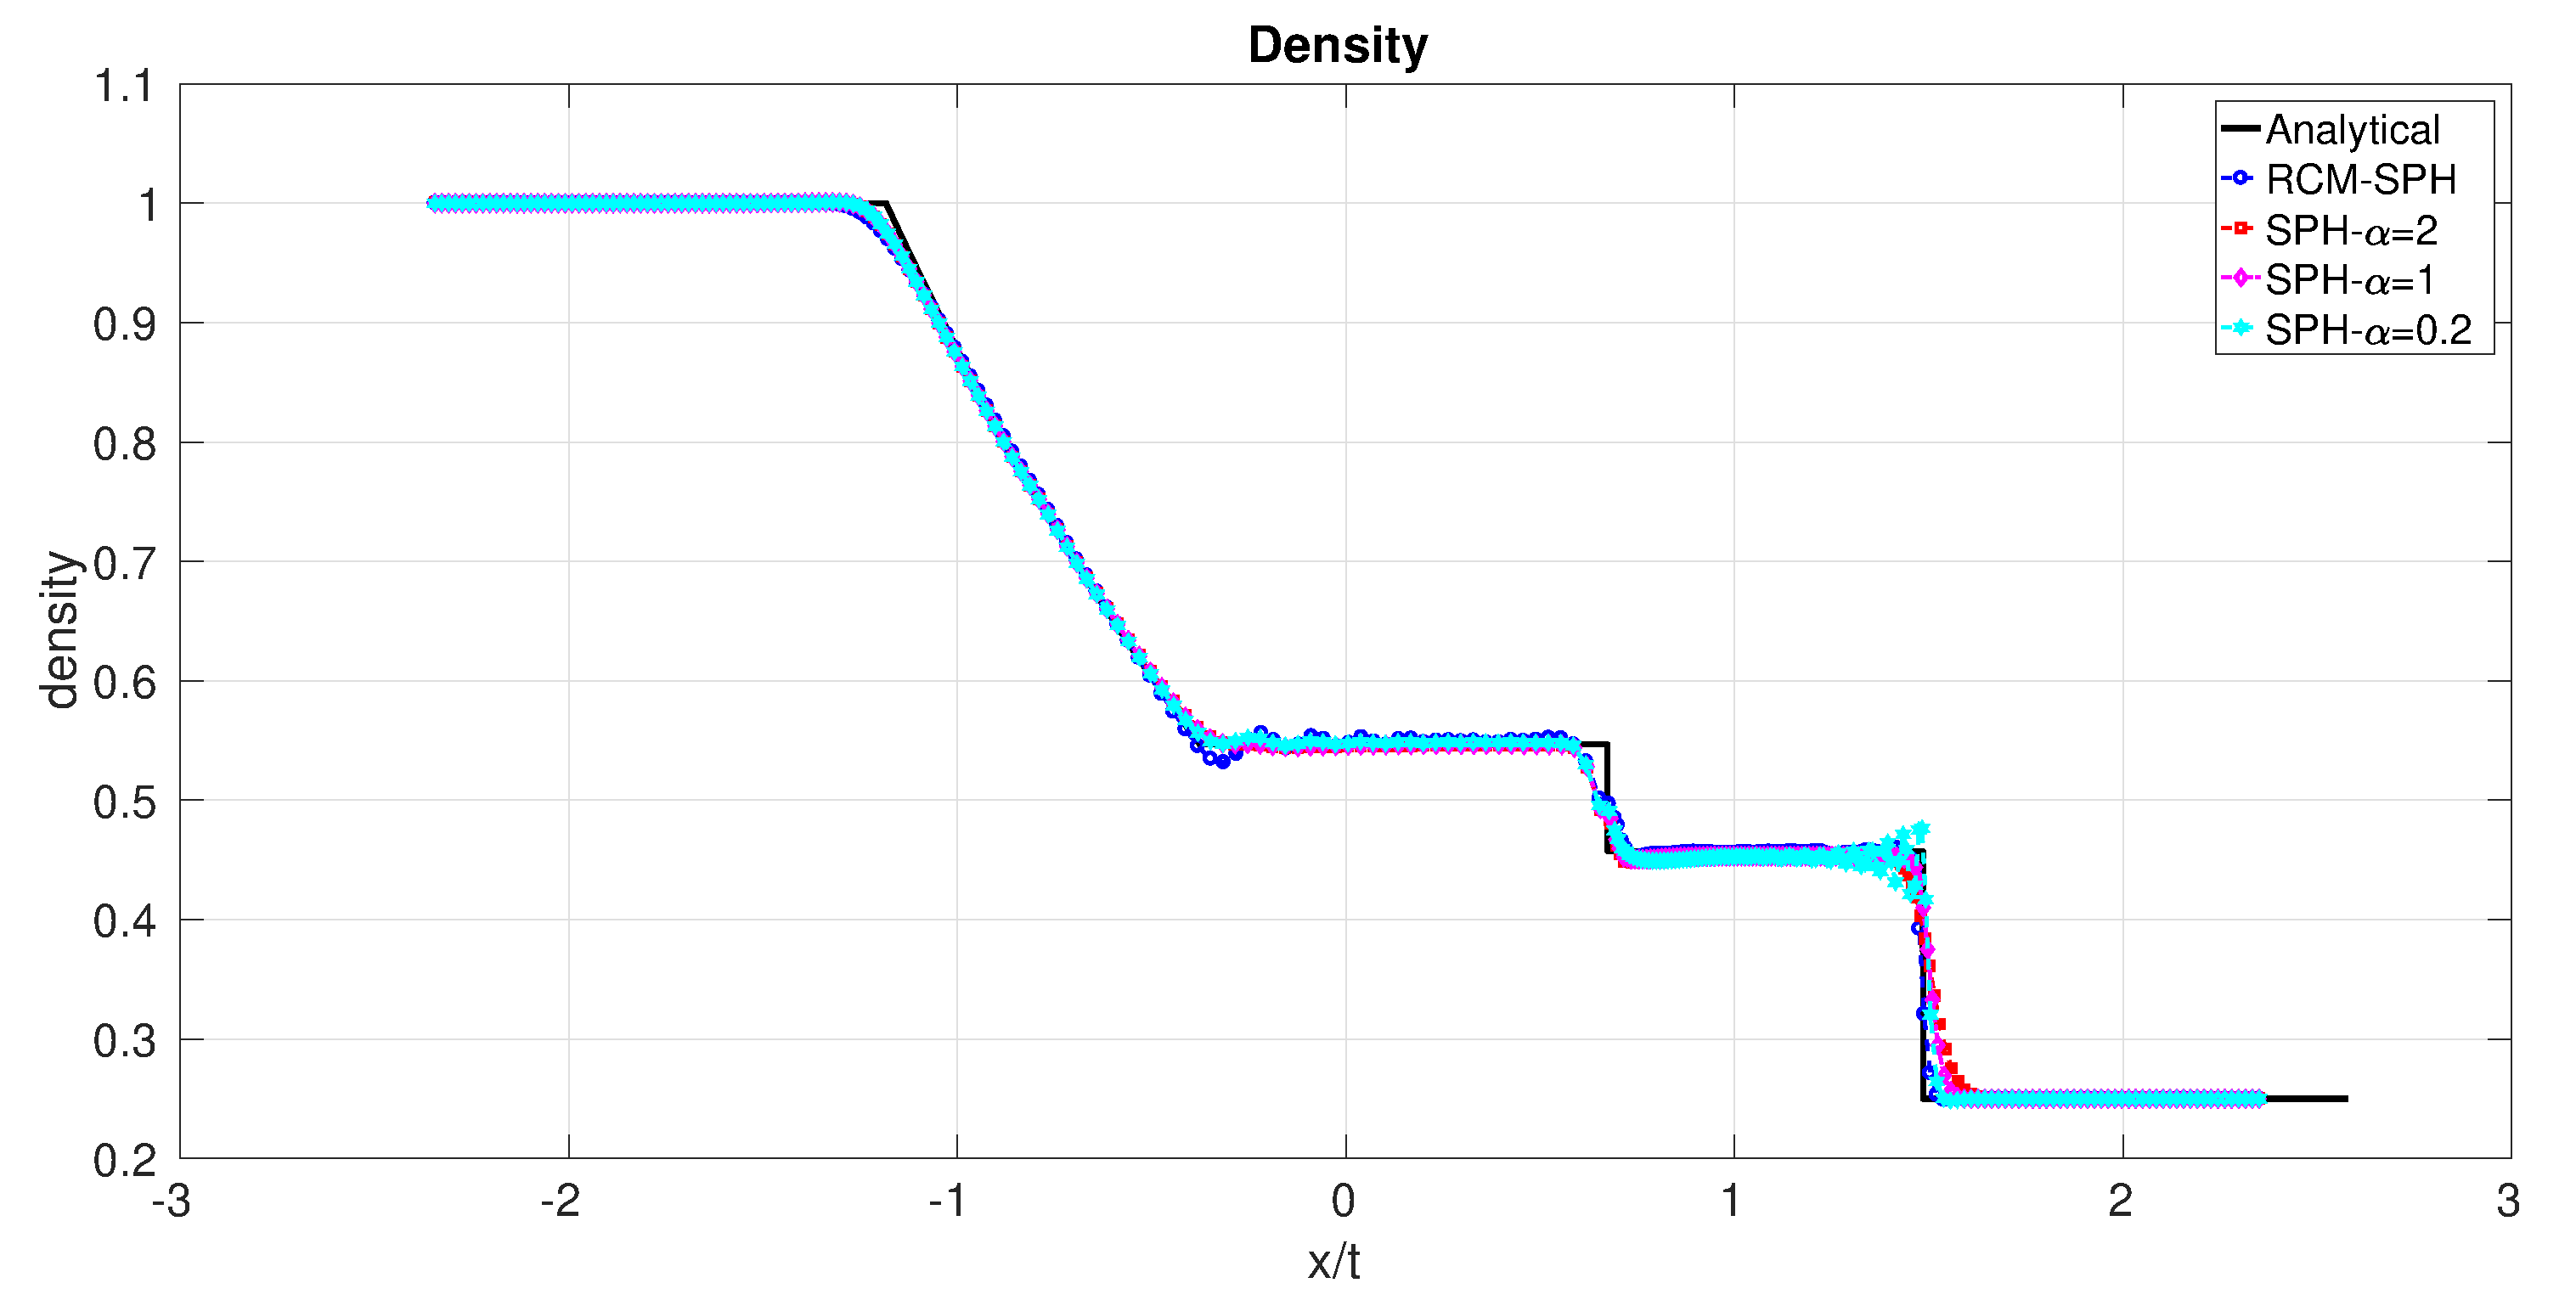
\includegraphics[width=0.99 \textwidth]{./Figures/Sod/RCM-Sod-SPH-alf-rho}
    \end{minipage}%
    \begin{minipage}{.495 \textwidth}
        \centering
        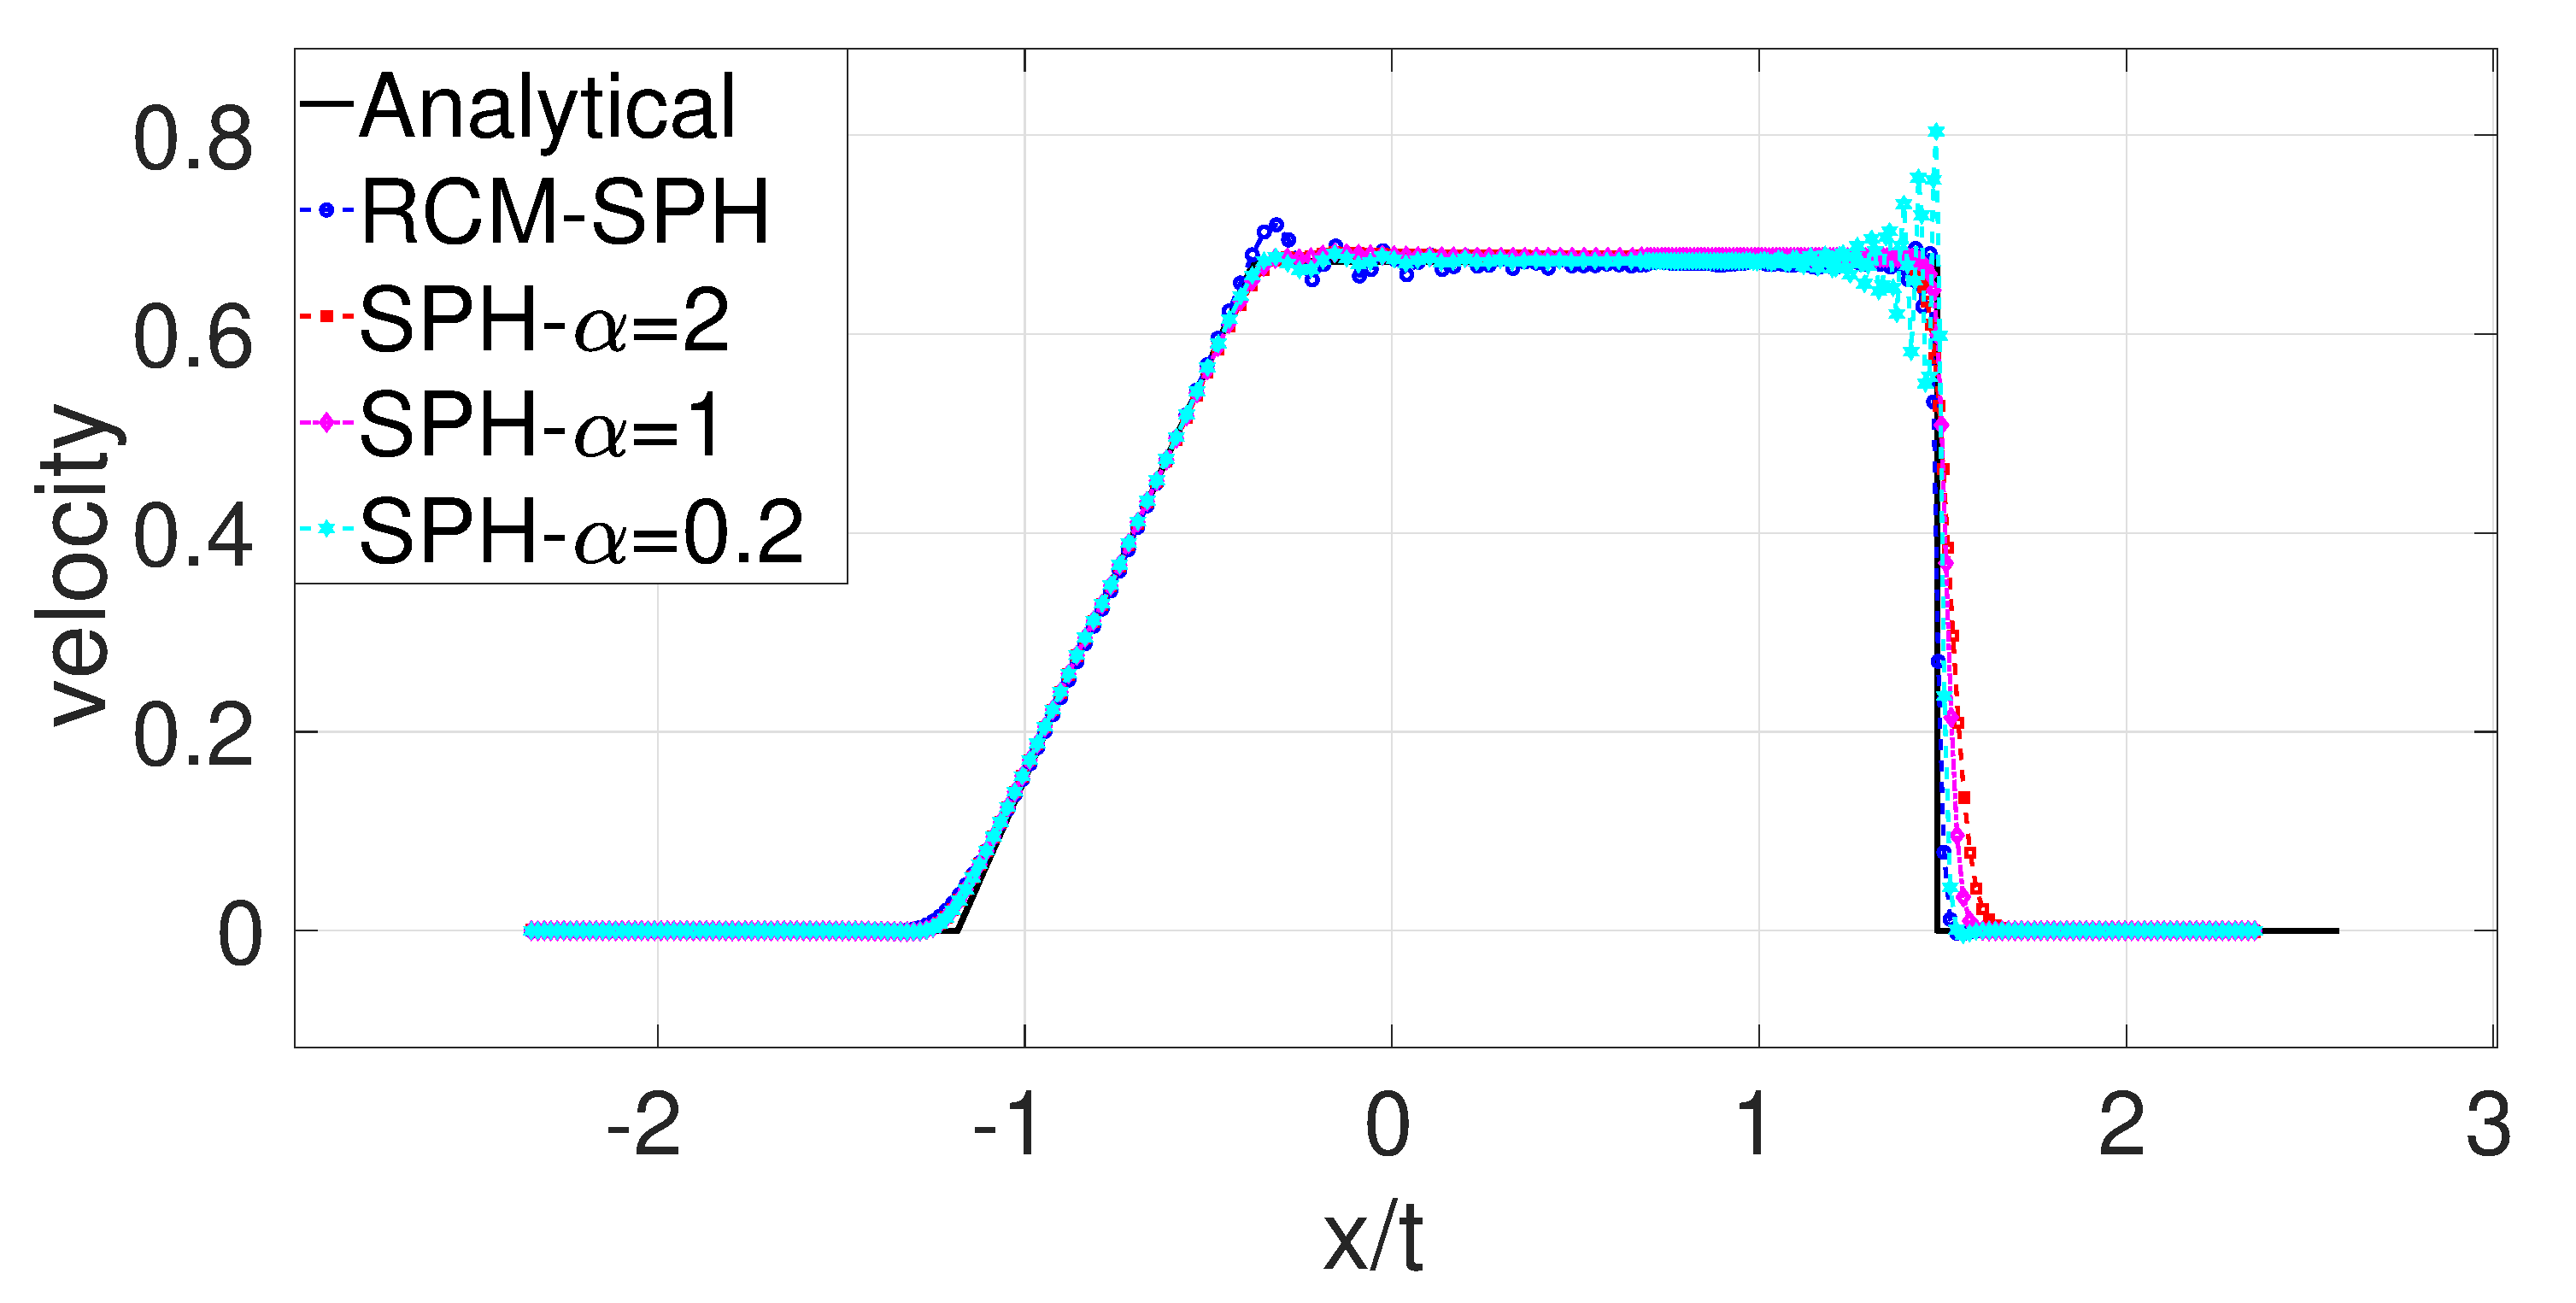
\includegraphics[width=0.99 \textwidth]{./Figures/Sod/RCM-Sod-SPH-alf-v}
    \end{minipage}%
    \\
    \begin{minipage}{.495\textwidth}
        \centering
        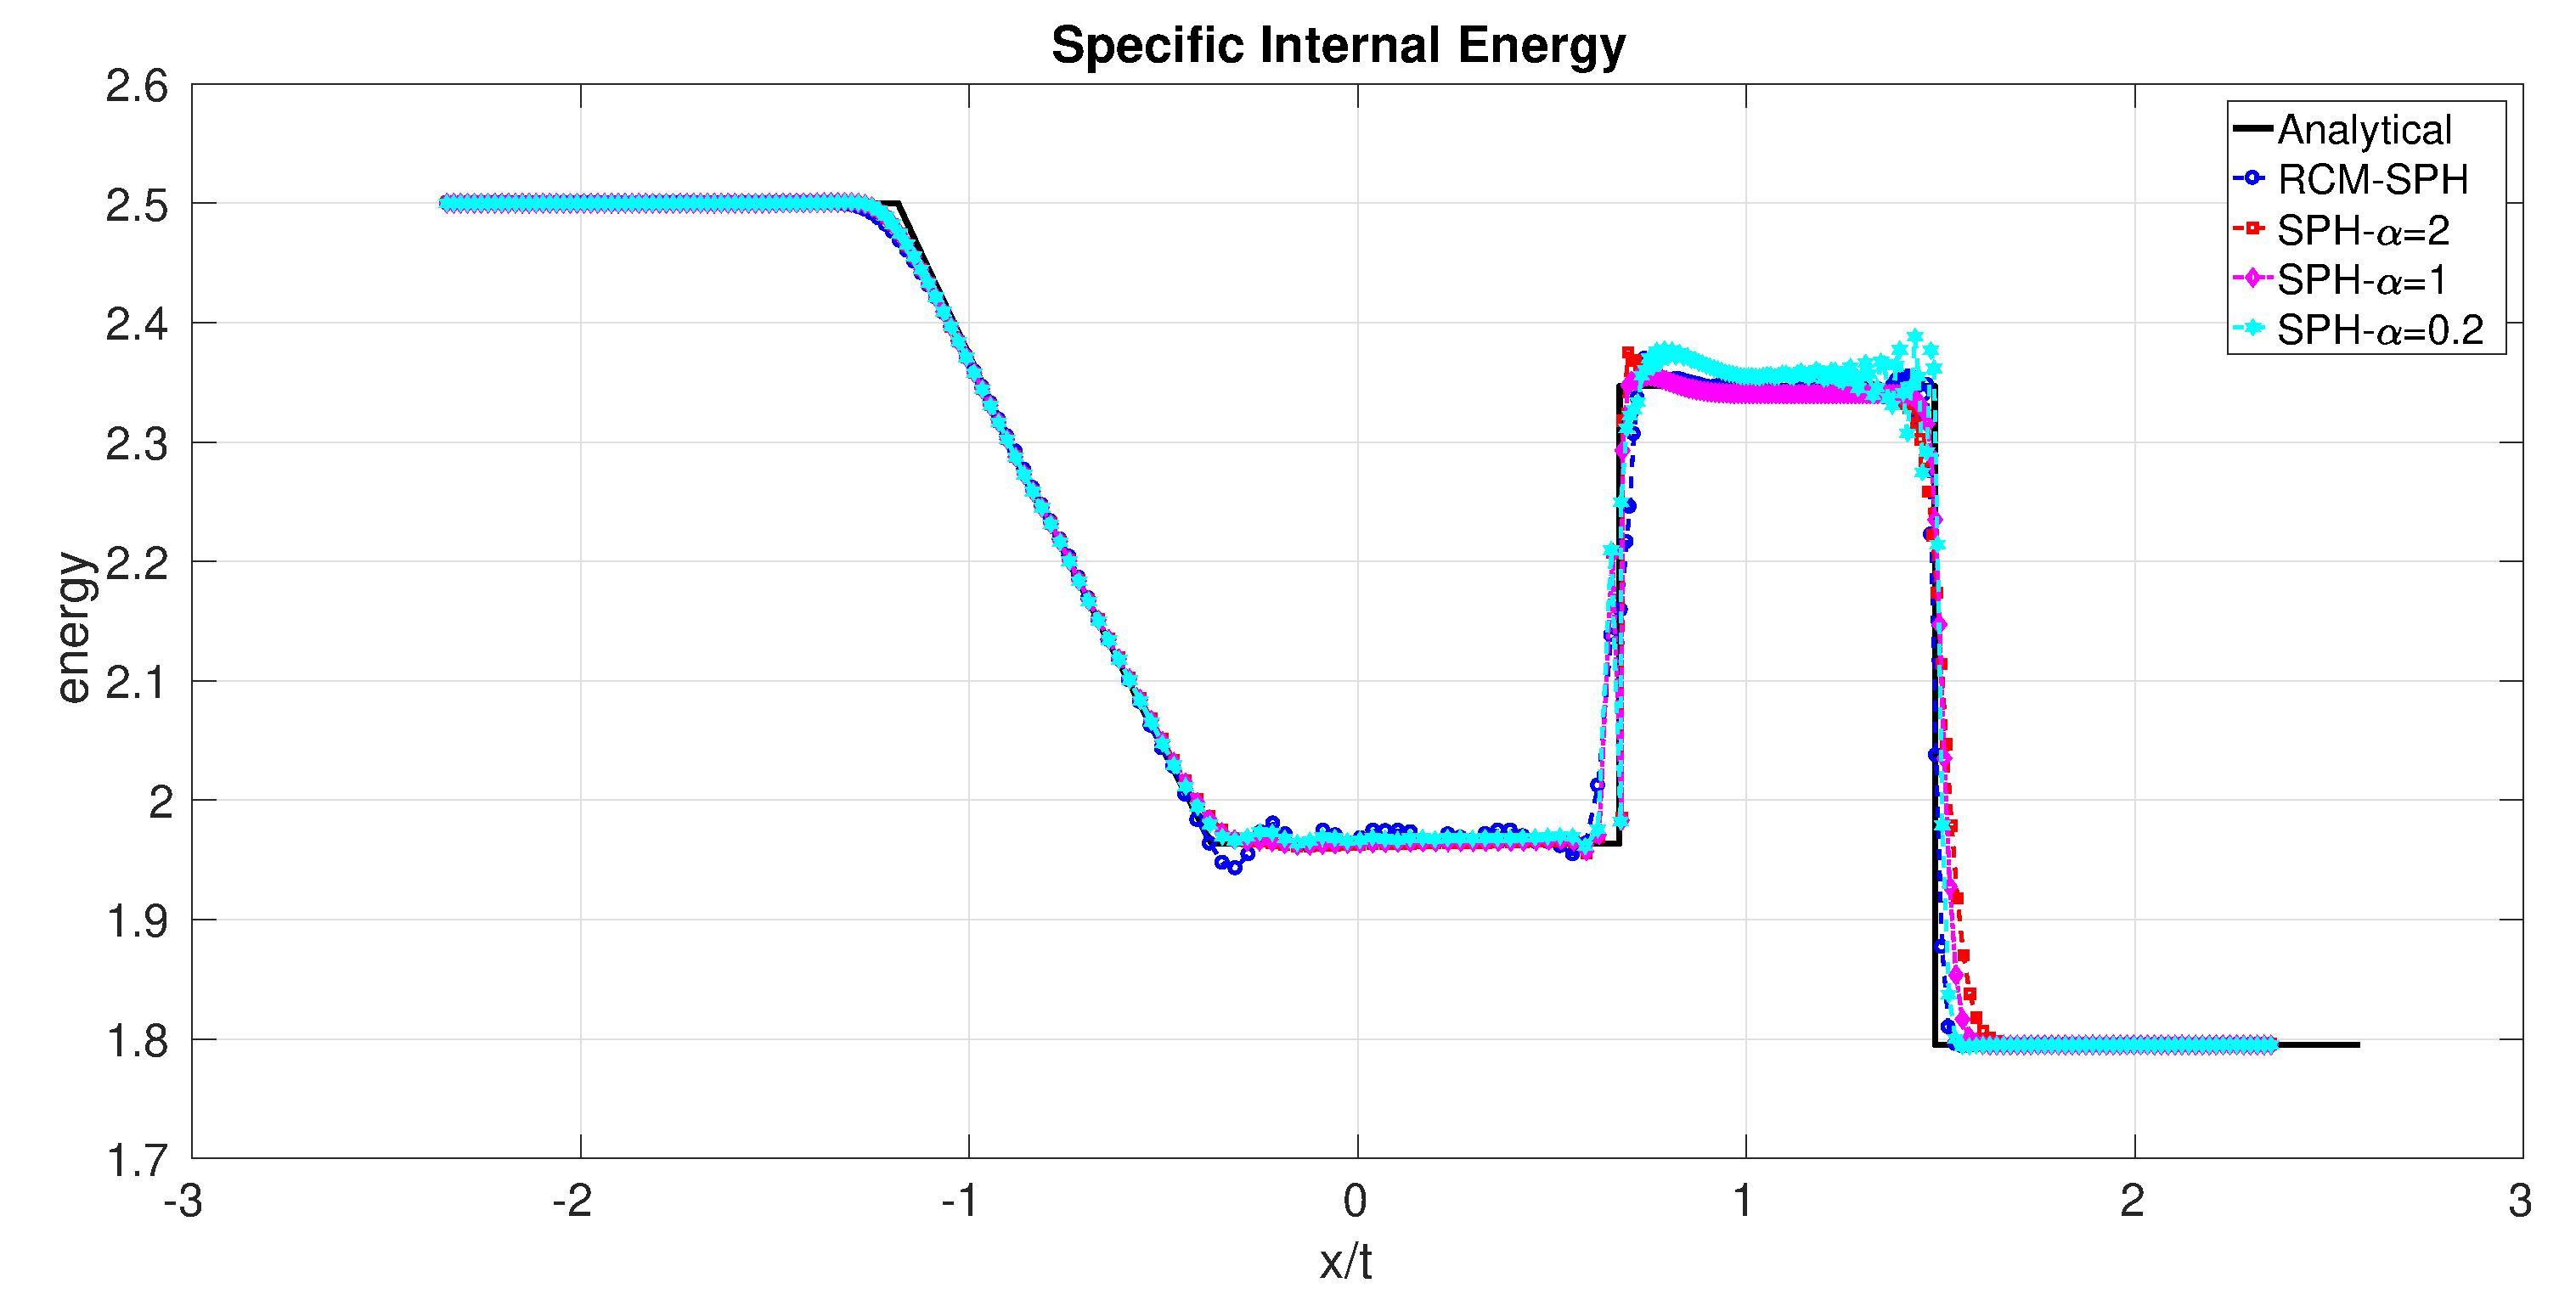
\includegraphics[width=0.99 \textwidth]{./Figures/Sod/RCM-Sod-SPH-alf-e}
    \end{minipage}%
    \begin{minipage}{.495 \textwidth}
        \centering
        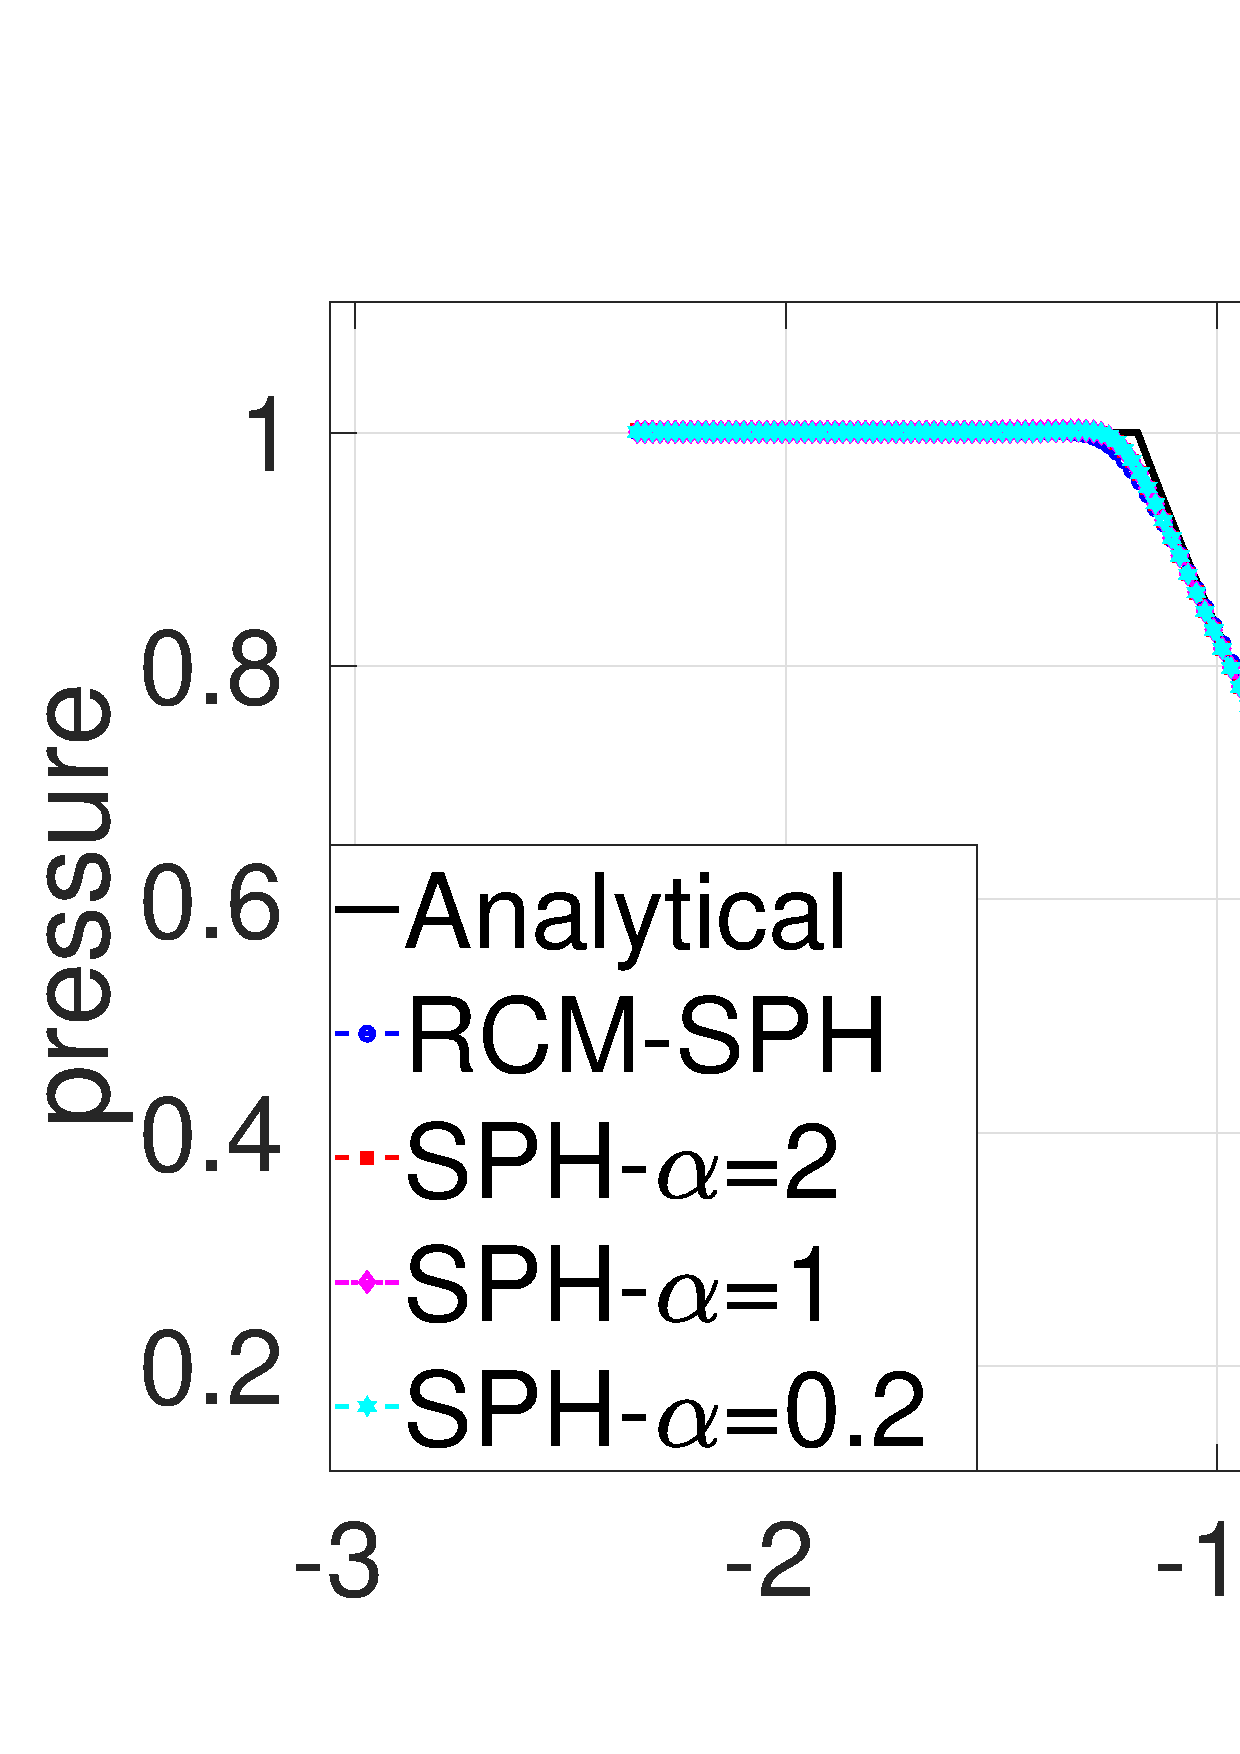
\includegraphics[width=0.99 \textwidth]{./Figures/Sod/RCM-Sod-SPH-alf-p}
    \end{minipage}% 
    \\
    \begin{minipage}{.495\textwidth}
        \centering
        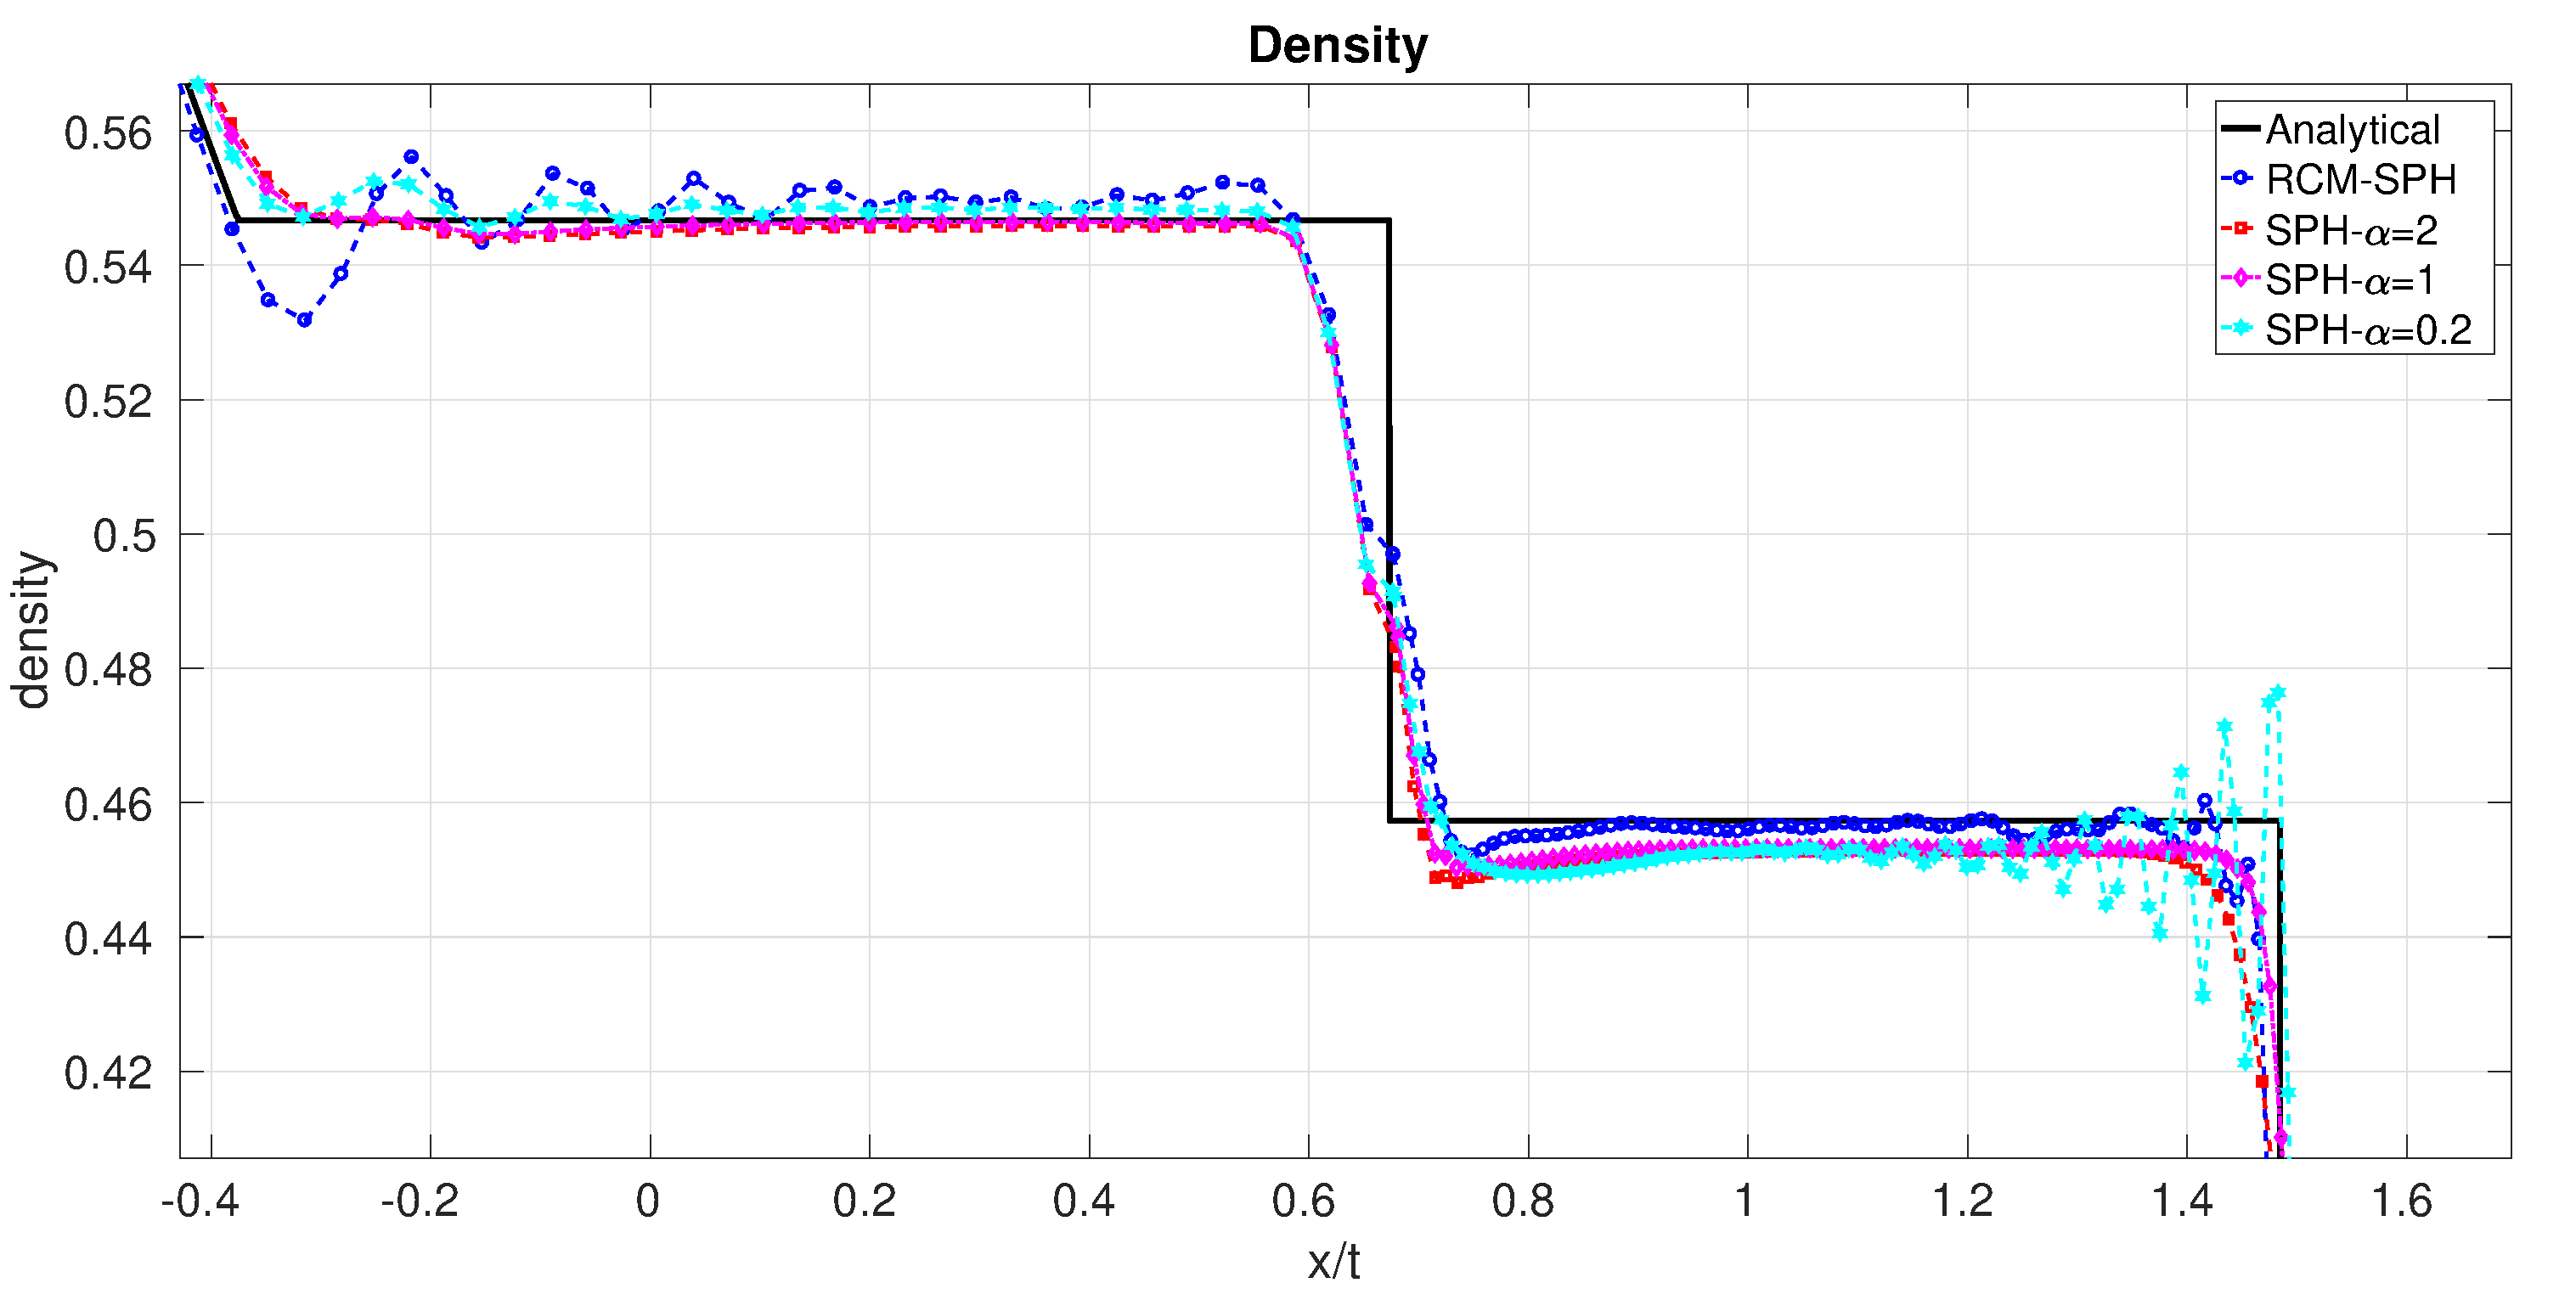
\includegraphics[width=0.99 \textwidth]{./Figures/Sod/RCM-Sod-SPH-alf-rho-zoom}
    \end{minipage}%
    \begin{minipage}{.495 \textwidth}
        \centering
        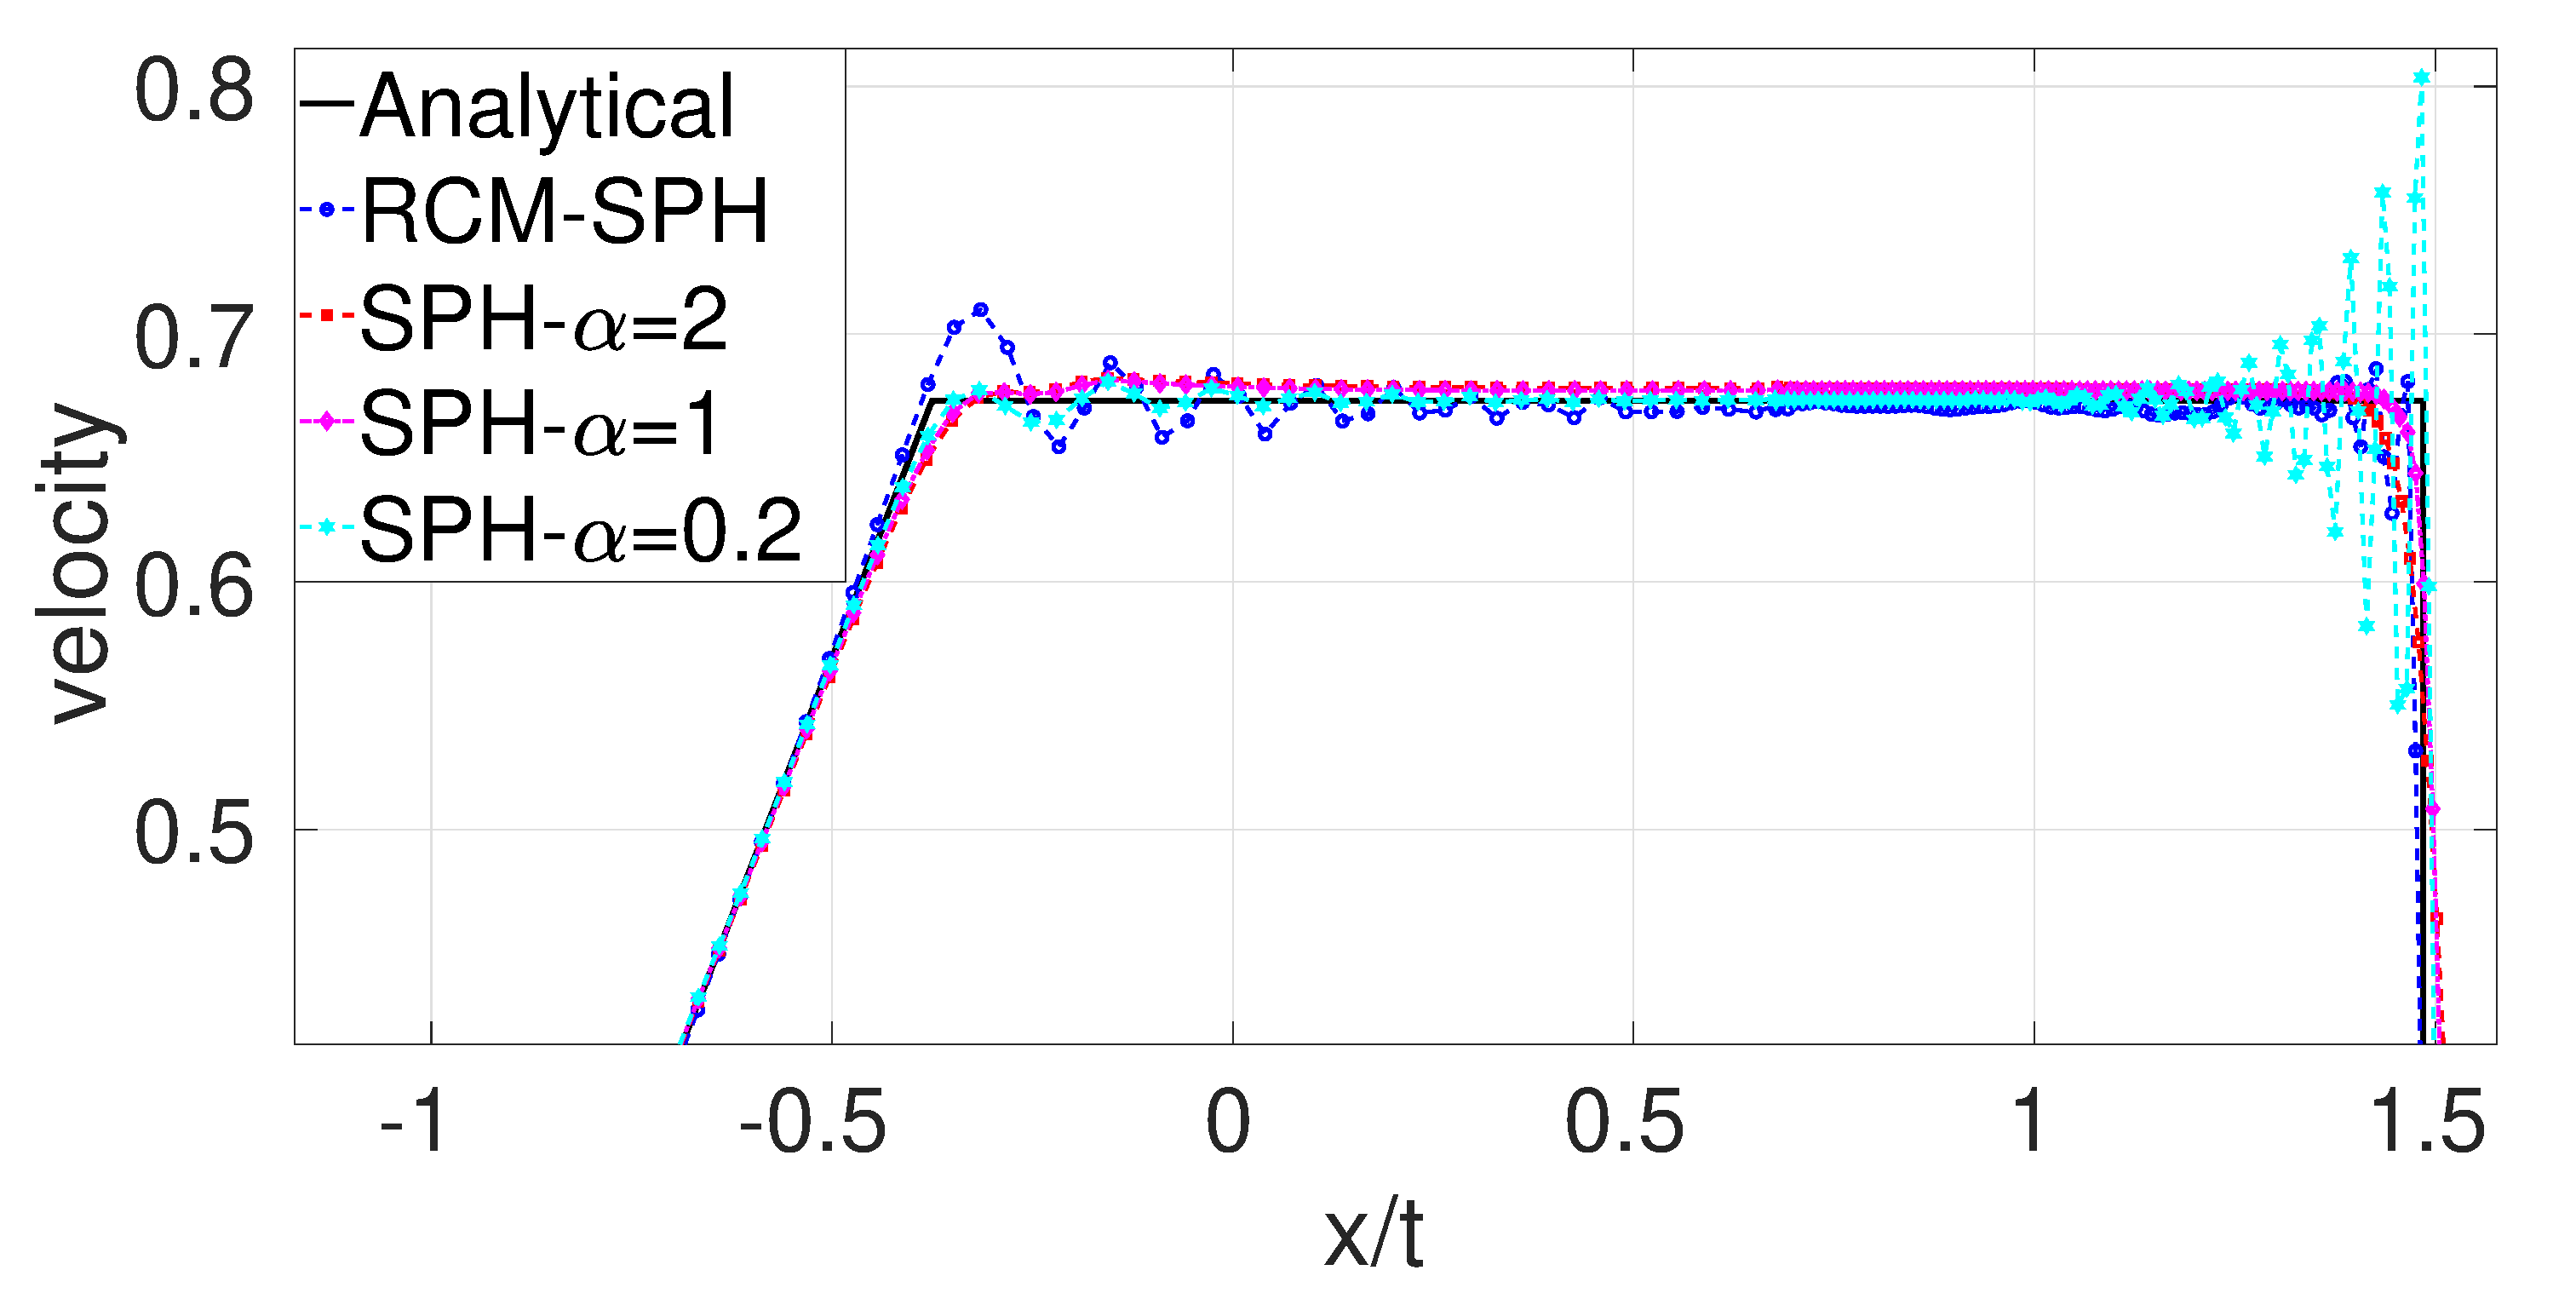
\includegraphics[width=0.99 \textwidth]{./Figures/Sod/RCM-Sod-SPH-alf-v-zoom}
    \end{minipage}% 
    \\
    \begin{minipage}{.495 \textwidth}
        \centering
        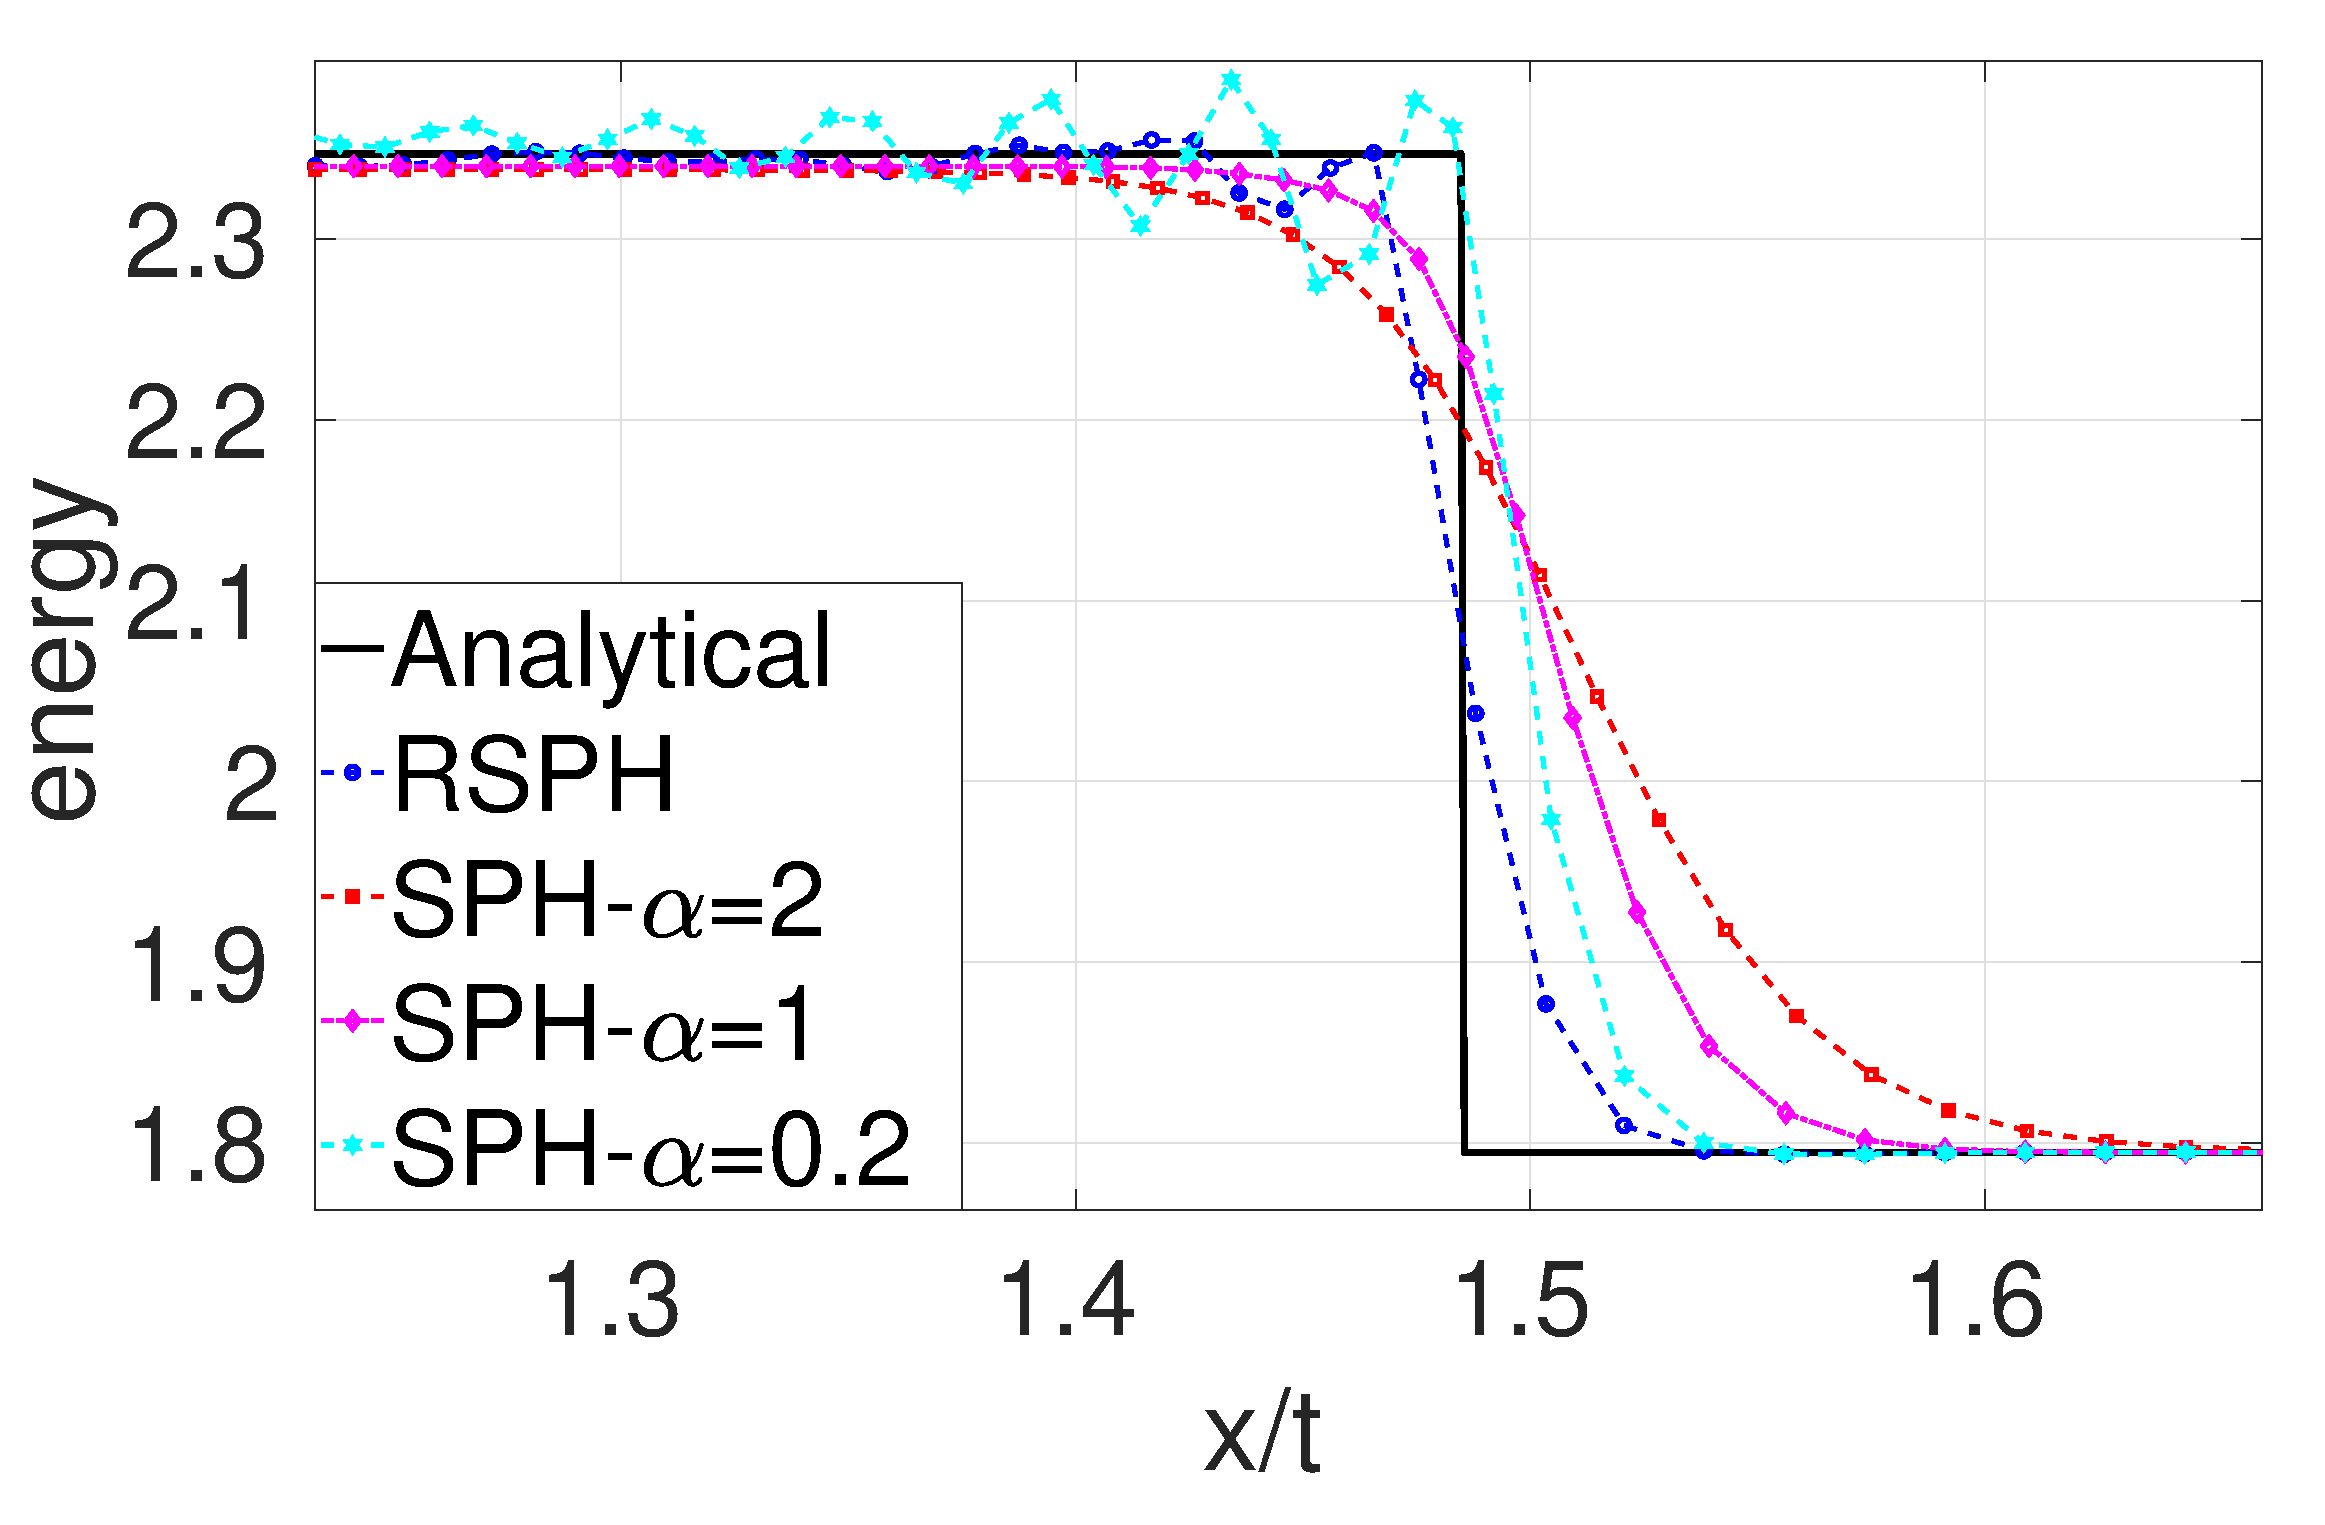
\includegraphics[width=0.99 \textwidth]{./Figures/Sod/RCM-Sod-SPH-alf-e-zoom}
    \end{minipage}% 
    \begin{minipage}{.495\textwidth}
        \centering
        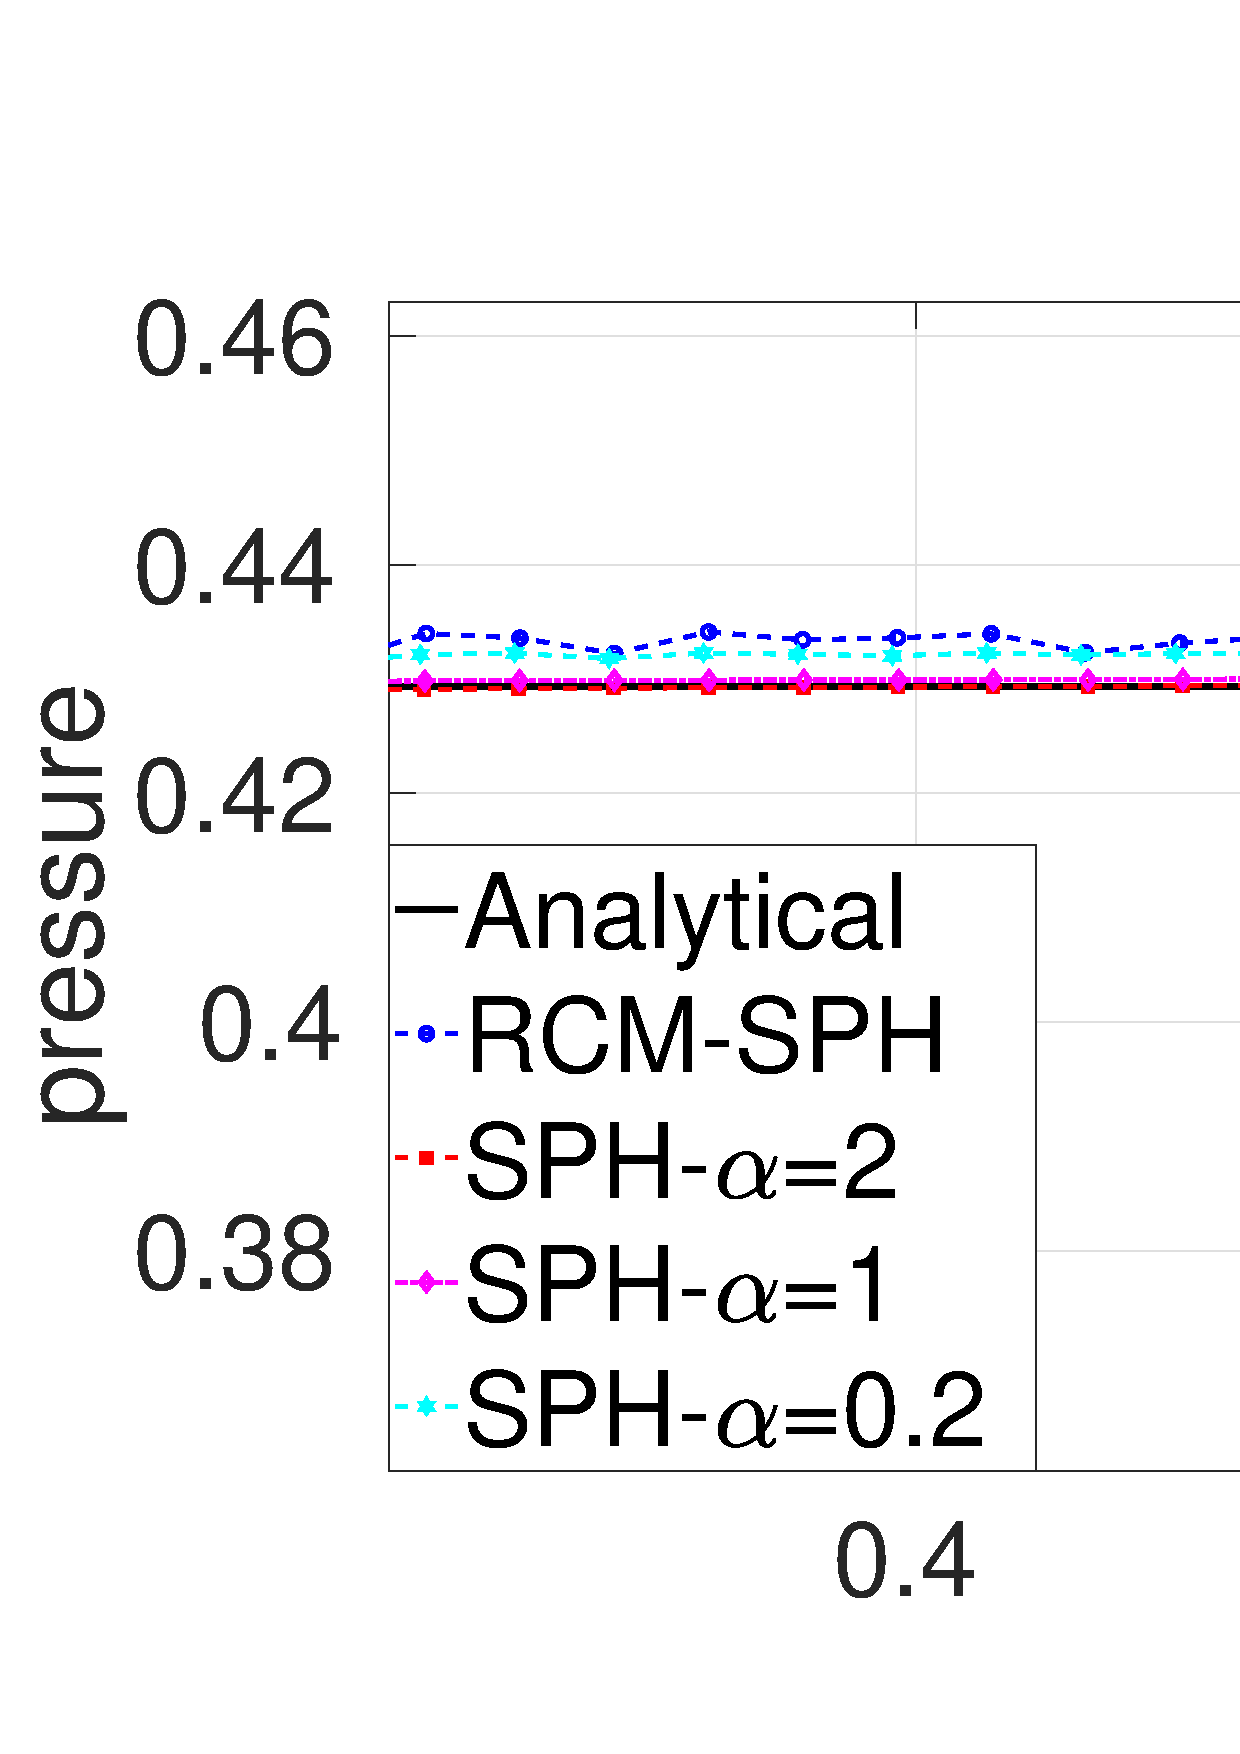
\includegraphics[width=0.99 \textwidth]{./Figures/Sod/RCM-Sod-SPH-alf-p-zoom}
    \end{minipage}%    
    \caption{Comparison of RSPH with SPH using different artificial viscosity coefficients. Artificial viscosity coefficients are choosen to always satisfy: $\beta=2\alpha$ in all SPH tests. The last four plots are zoomed views. There is almost no fluctuation when $\alpha=1$ and $\alpha=2$, illustrating that numerical fluctuation is completely suppressed if artificial viscosity is large enough. Zoomed view of density shows that the fluctuations in the area away from shock for "RSPH" are more obvious than those for "$SPH-\alpha=0.2$", implying that RSPH introduces smaller artificial viscosity than "$\alpha=0.2$" in the area far away from shock. However, fluctuations around shock is much more obvious for "$\alpha=0.2$" than RSPH, implying that RSPH introduces larger artificial viscosity than "$\alpha=0.2$" around shock. To summarize, the equivalent artificial viscosity in RSPH is adaptive. Similar conclusion can be drew from zoomed view of velocity. The third zoomed view shows different degrees of smearing at the shock. The larger the artificial viscosity, the less sharp the solution at the shock. Since "$\alpha=0.2$" is sharper than "RSPH" at the shock, "$\alpha=0.2$" introduces less dissipation at the shock, which is consisitent with information implied by zoomed view of density. "$\alpha=1.0$" and "$\alpha=2.0$" introduces more dissipation than "RSPH" in the area around the shock. The last zoomed view shows pressure around the contact discontinuity. It shows that RSPH get rid of pressure "wiggle" around the contact discontinuity.}
    \label{fig:RCM-Sod-SPH-alf}
\end{figure}

Test 1 is simulated using standard SPH with different artificial viscosity coeffients, GSPH and RSPH. RSPH is compared with SPH using different artificial viscosity coefficients in Fig. \ref{fig:RCM-Sod-SPH-alf}. In all simulation, the artificial viscosity $\beta$ is set to be twice of $\alpha$. For example, for the test "$SPH-\alpha=2$", $\beta=4$. Several interesting observation are made based on the comparison.
First of all, by adding artificial viscosity SPH introduces dissipation that decays the numerical fluctuations. large artificial viscosity in SPH can reduce Numerical fluctuations can be suppressed completely when large enough dissipation is introduced.
%The mechanism for SPH to reduce (or completely get rid of) fluctuations should be completely different from that of new adaptive method of smoothing length. 
%The new adaptive method, reduces the sources of such fluctuations.
Secondly, the equivalent artificial viscosity coefficients introduced by RSPH varies adaptively.
As shown in Fig. \ref{fig:RCM-Sod-SPH-alf}, RSPH can adjust the artificial viscosity adaptively, assigning smaller artificial viscosity coefficients (equivalent $\alpha$ much less then 0.2) at the area far away from shock front and sufficient large artificial viscosity coefficients (equivalent $\alpha$ is about 1.0) around the shock. So RSPH is actually more adaptive than SPH.
Thirdly, RSPH introduces less smearing of the shock front compared with SPH using most commonly adopted artificial viscosity coefficients ($\alpha=1.0$, $\beta=2.0$).
The last but not the least, the pressure around "wiggle" around contact discontinuity is completely eliminated by RSPH. It has been shown that thermal conduction is essential to mitigate the spurious pressure "wiggle" at contact discontinuity in SPH \citep{monaghan1997sph, sigalotti2006shock, price2008modelling, price2012smoothed}. As for GSPH, it is reported that an implicit thermal conduction is introduced by Godunov's scheme and help suppress the anomaly \citep{puri2014approximate}. Since RCM share many common places with Godunov's method, it is not surprise that RSPH can also suppress the "wiggle" at contact discontinuity.

\begin{figure}[H]
    \centering
    \begin{minipage}{.495\textwidth}
        \centering
        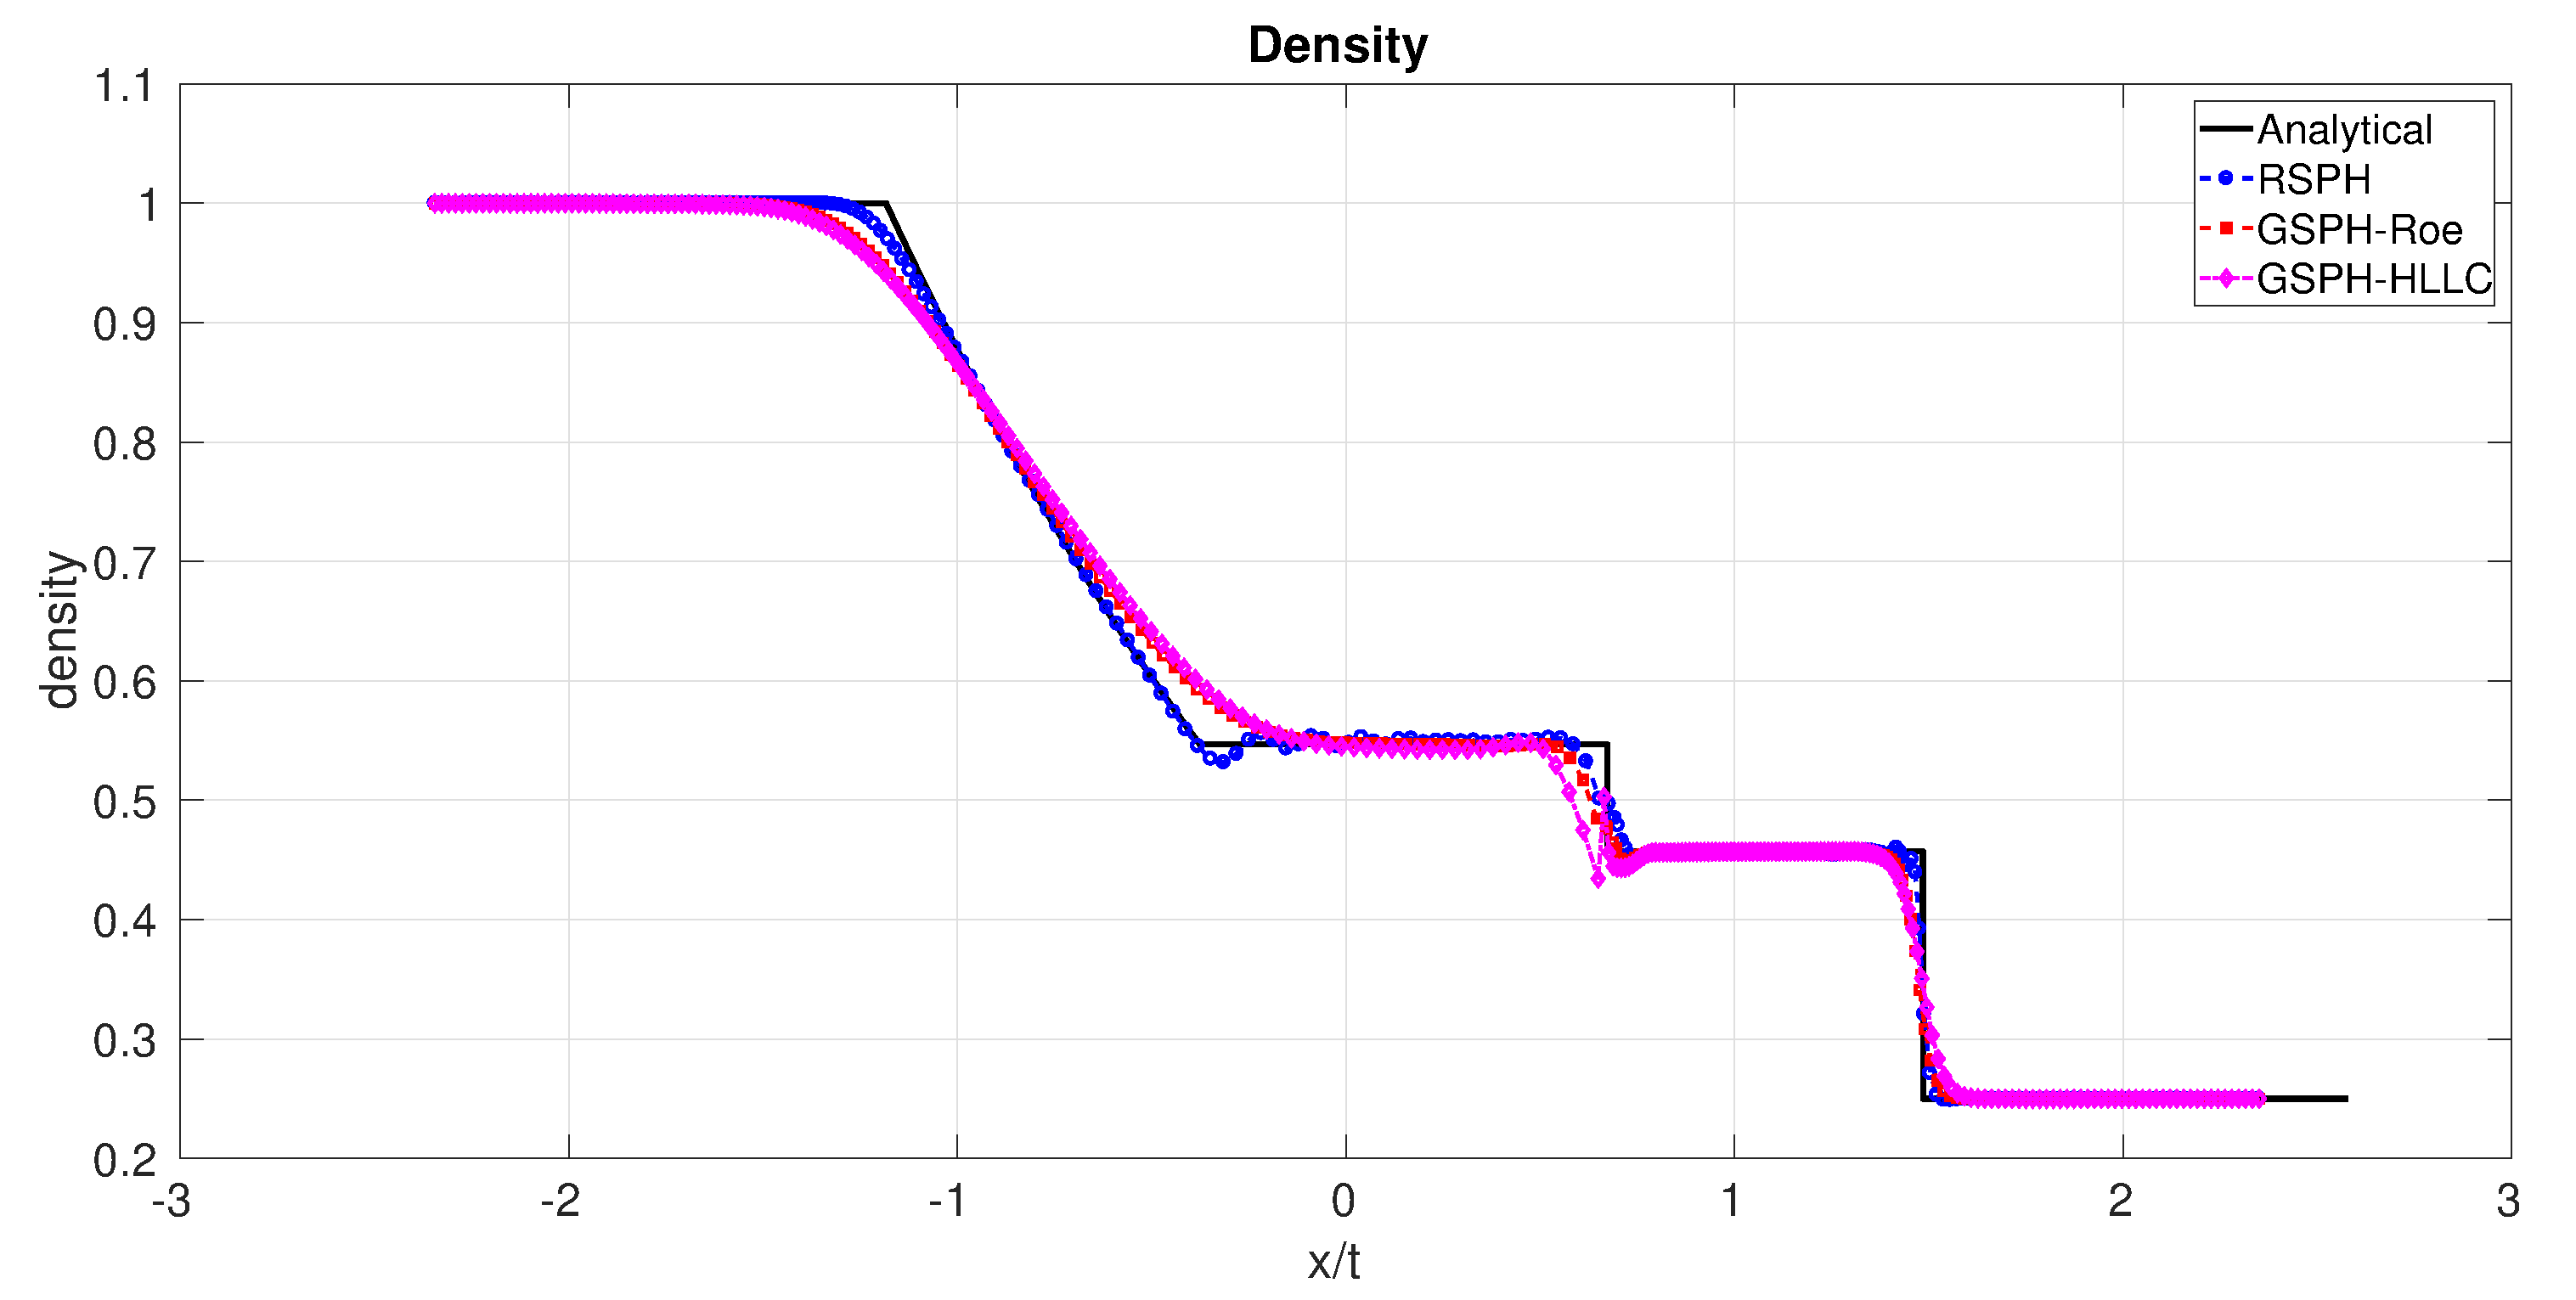
\includegraphics[width=0.99 \textwidth]{./Figures/Sod/RCM-Sod-GSPH-compare-rho}
    \end{minipage}%
    \begin{minipage}{.495 \textwidth}
        \centering
        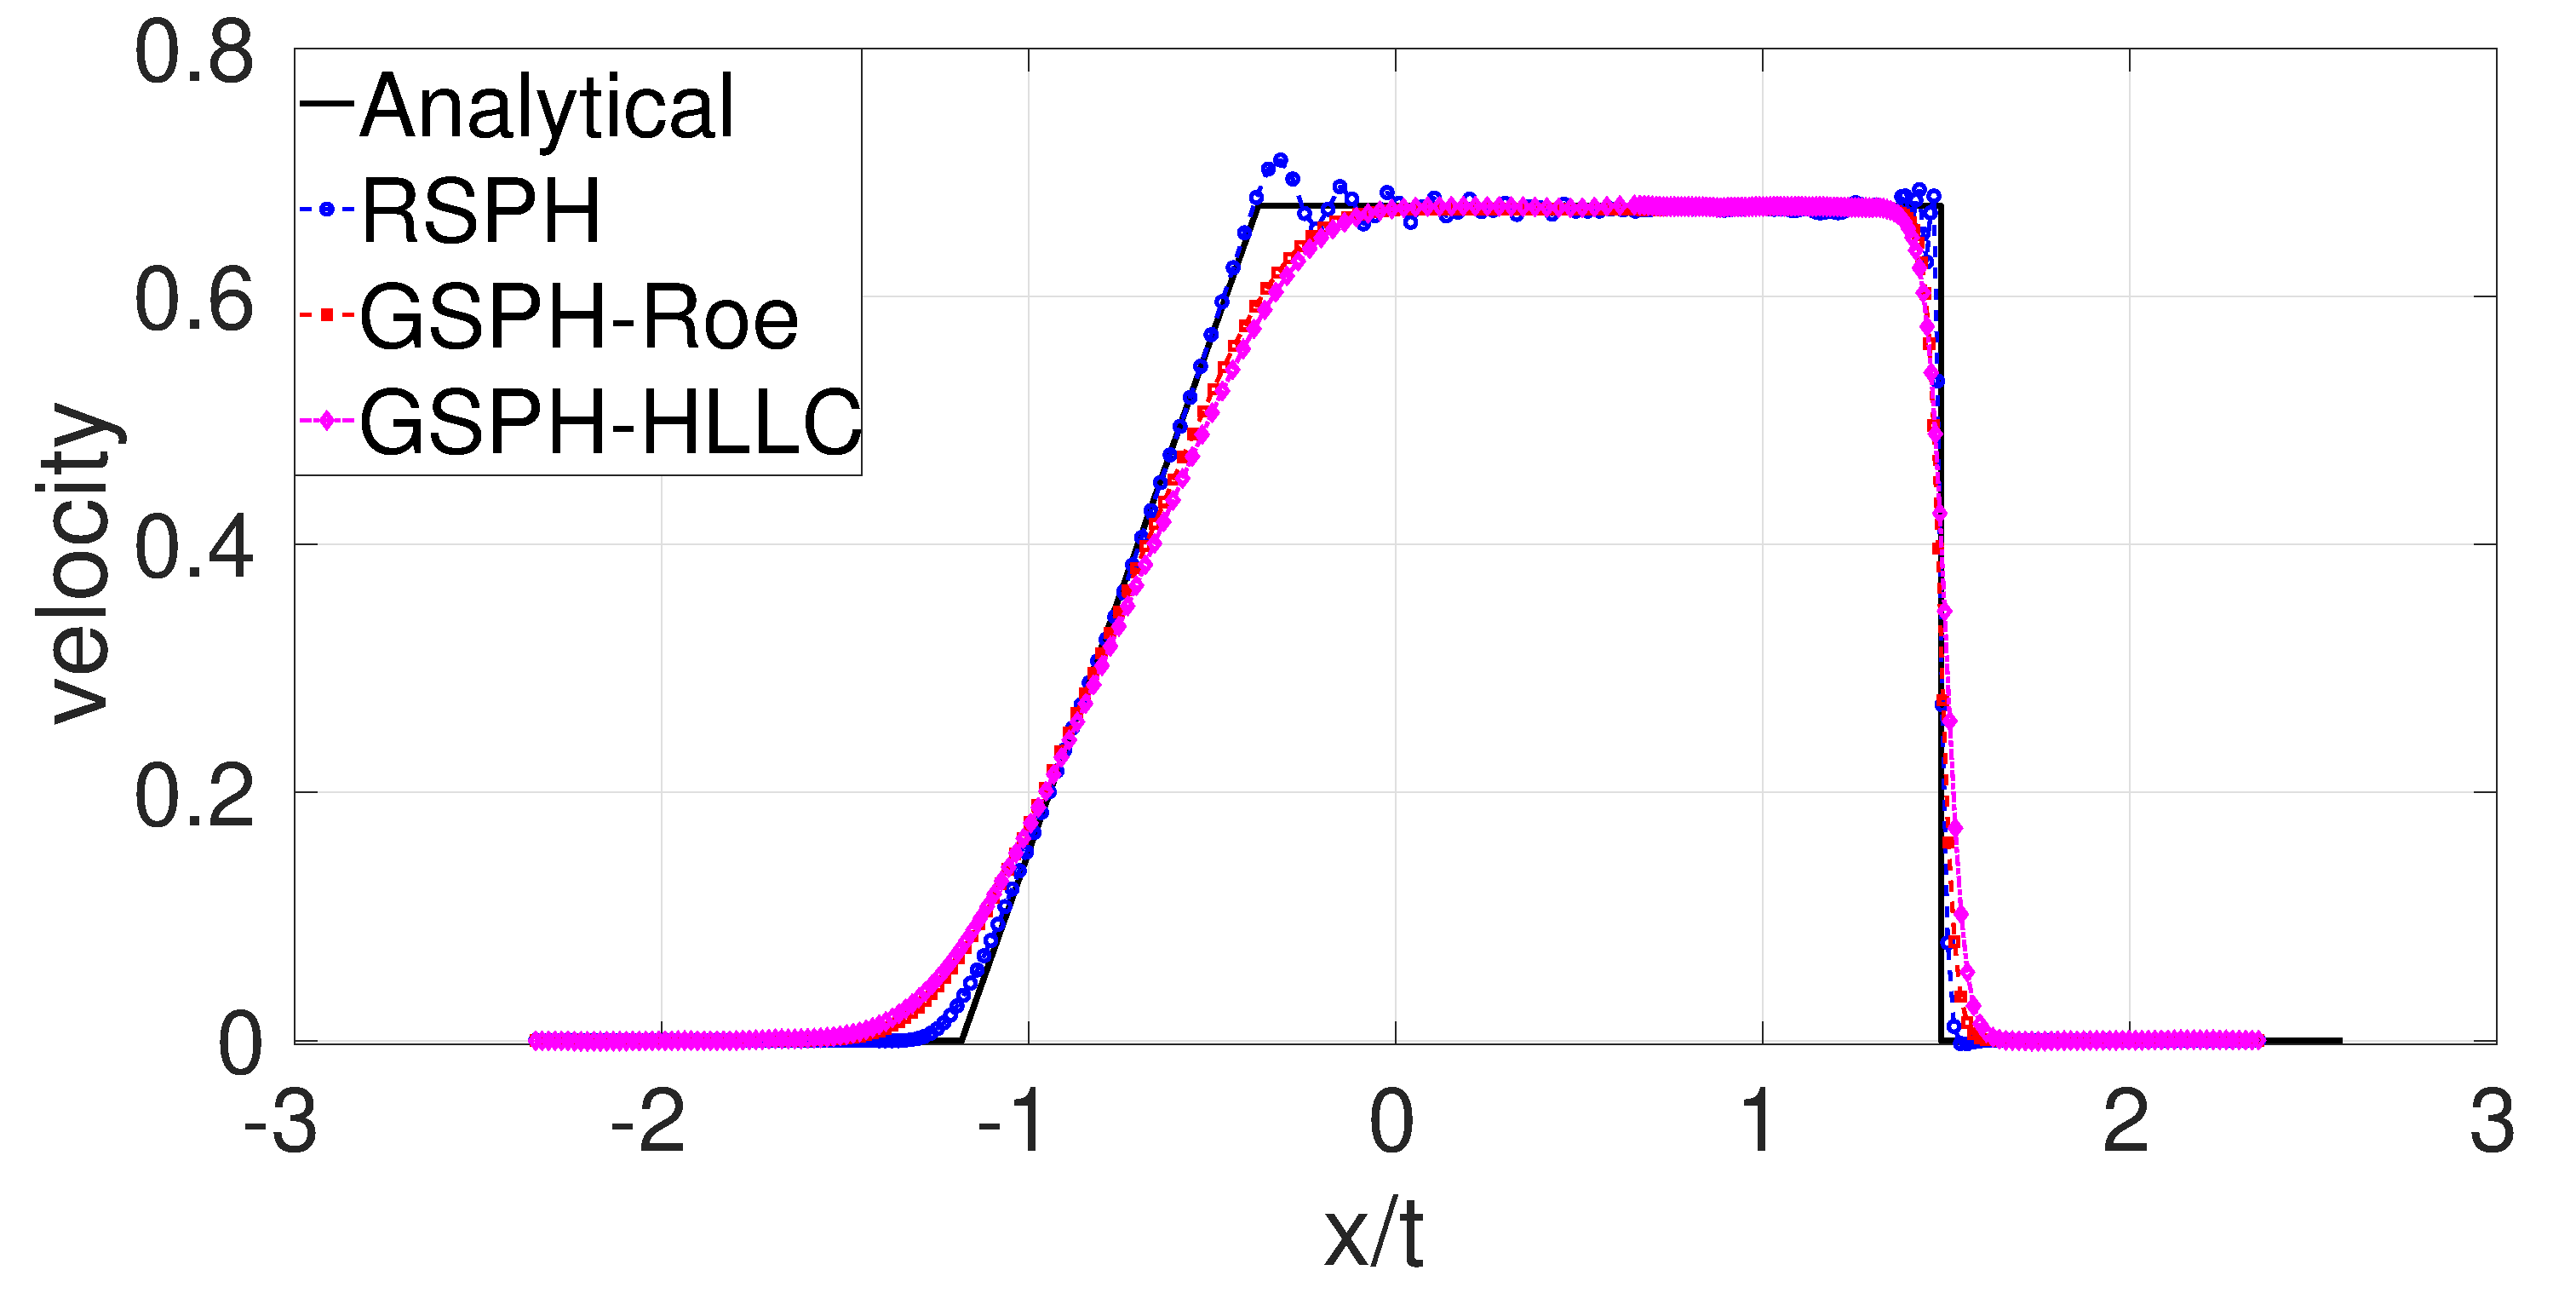
\includegraphics[width=0.99 \textwidth]{./Figures/Sod/RCM-Sod-GSPH-compare-v}
    \end{minipage}%
    \\
    \begin{minipage}{.495\textwidth}
        \centering
        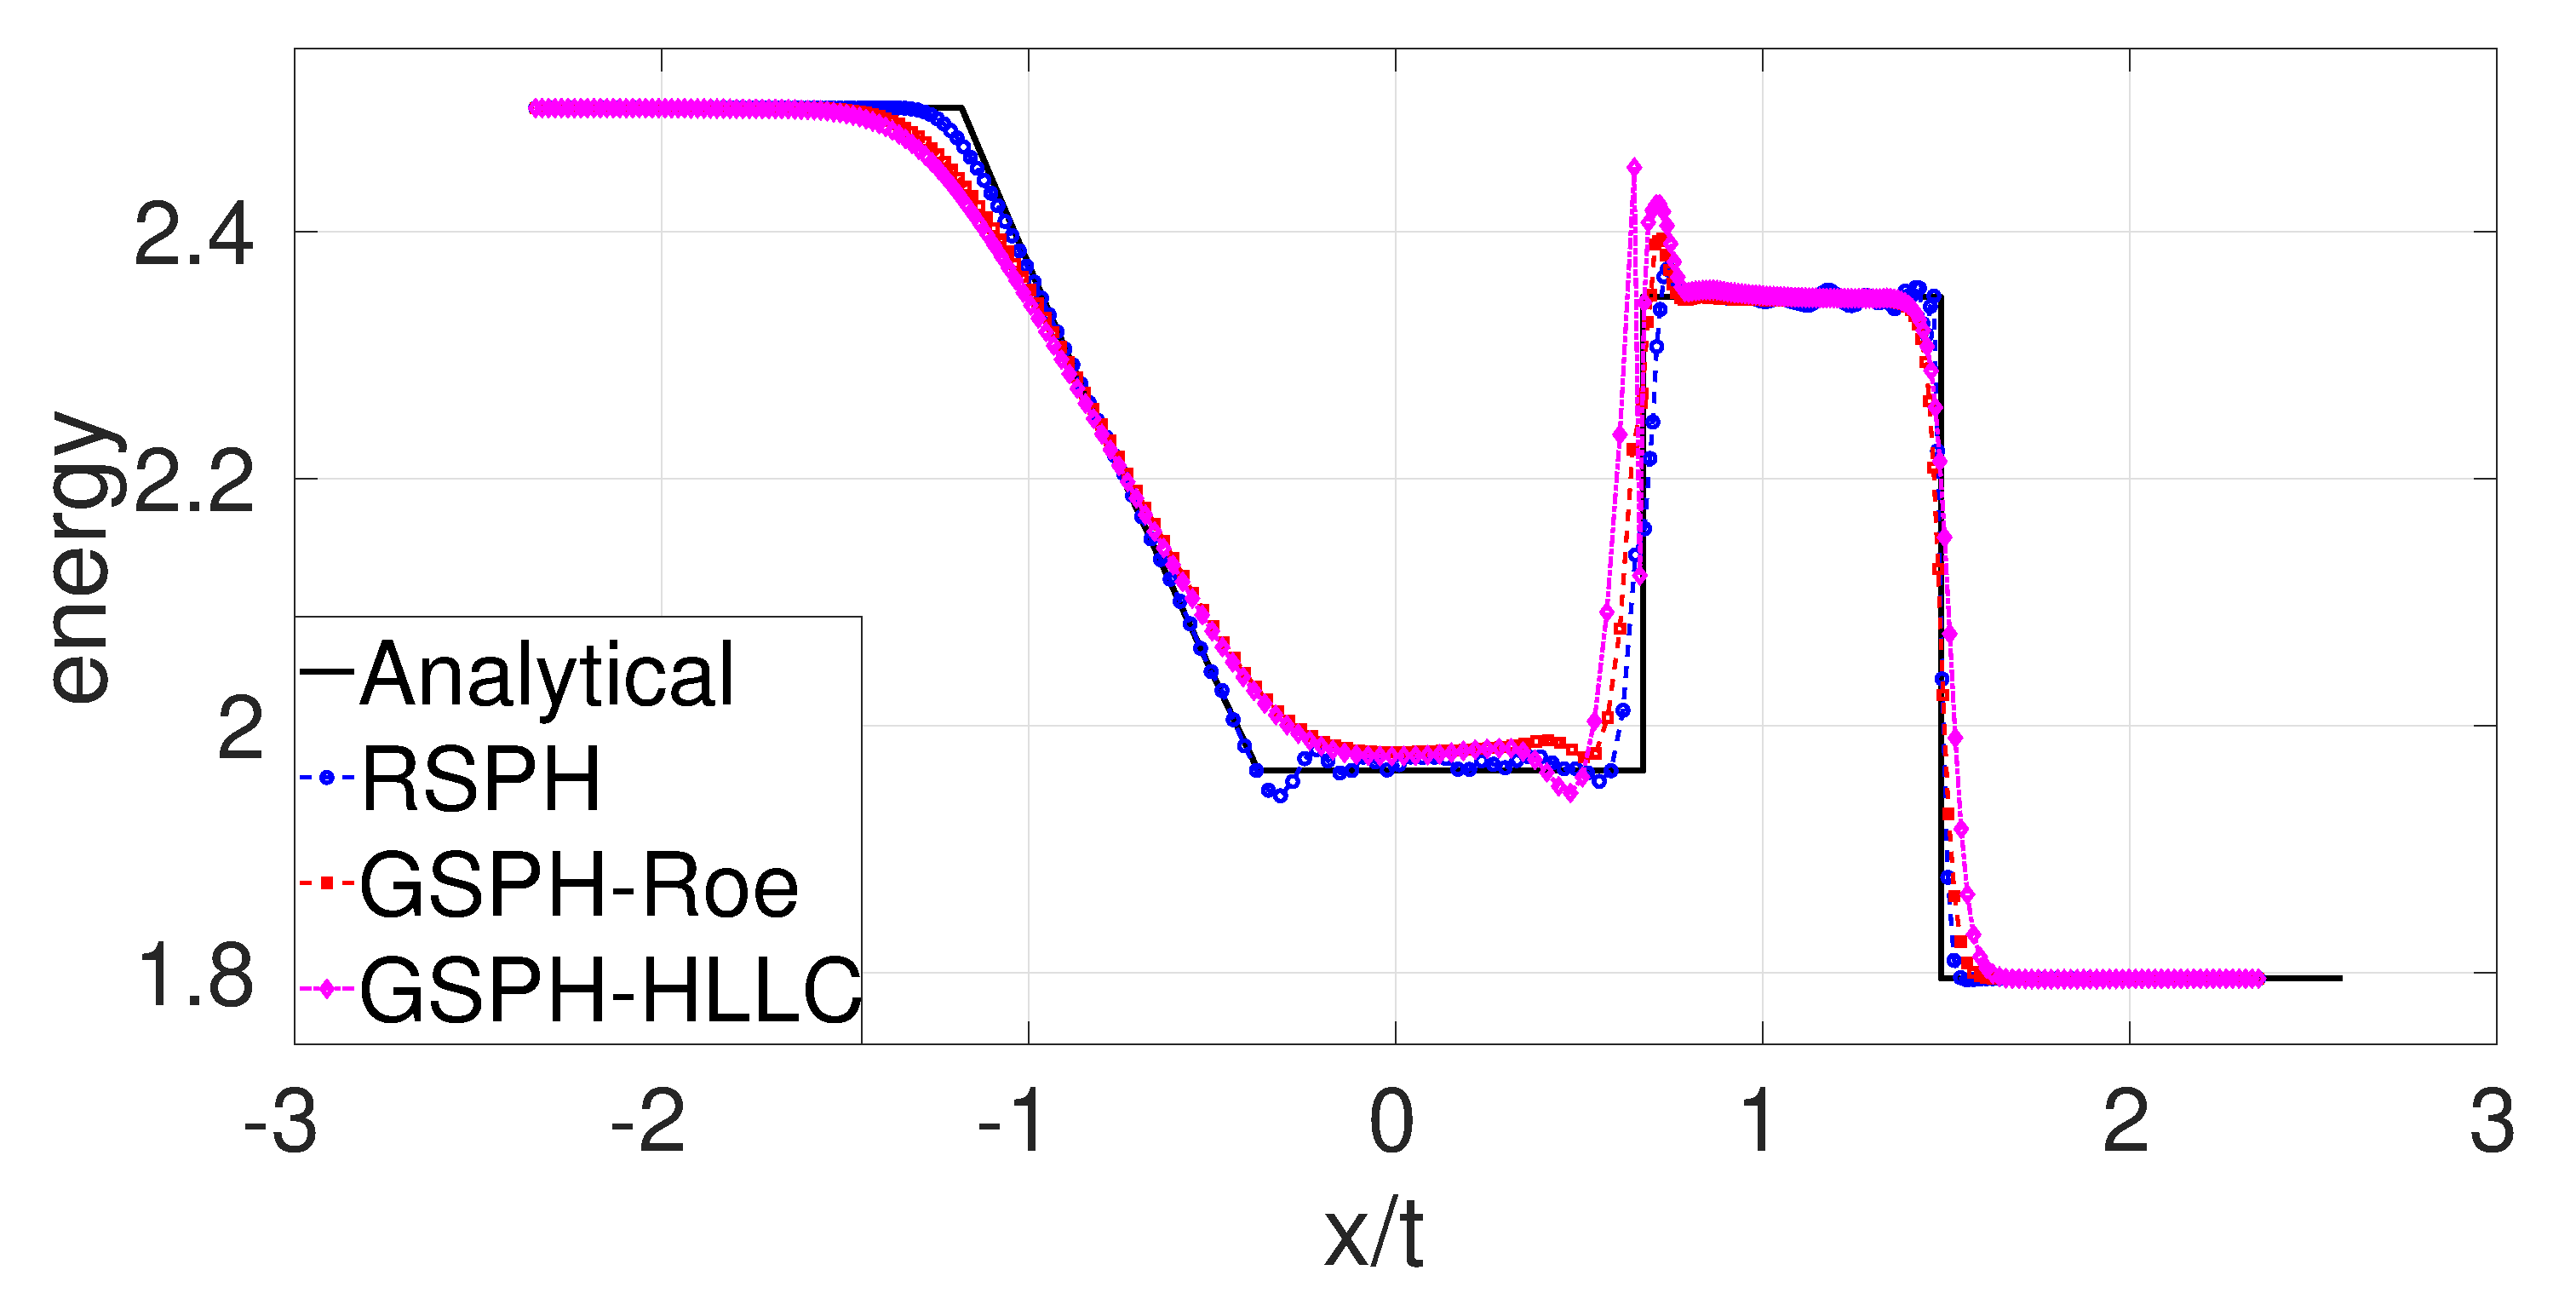
\includegraphics[width=0.99 \textwidth]{./Figures/Sod/RCM-Sod-GSPH-compare-e}
    \end{minipage}%
    \begin{minipage}{.495 \textwidth}
        \centering
        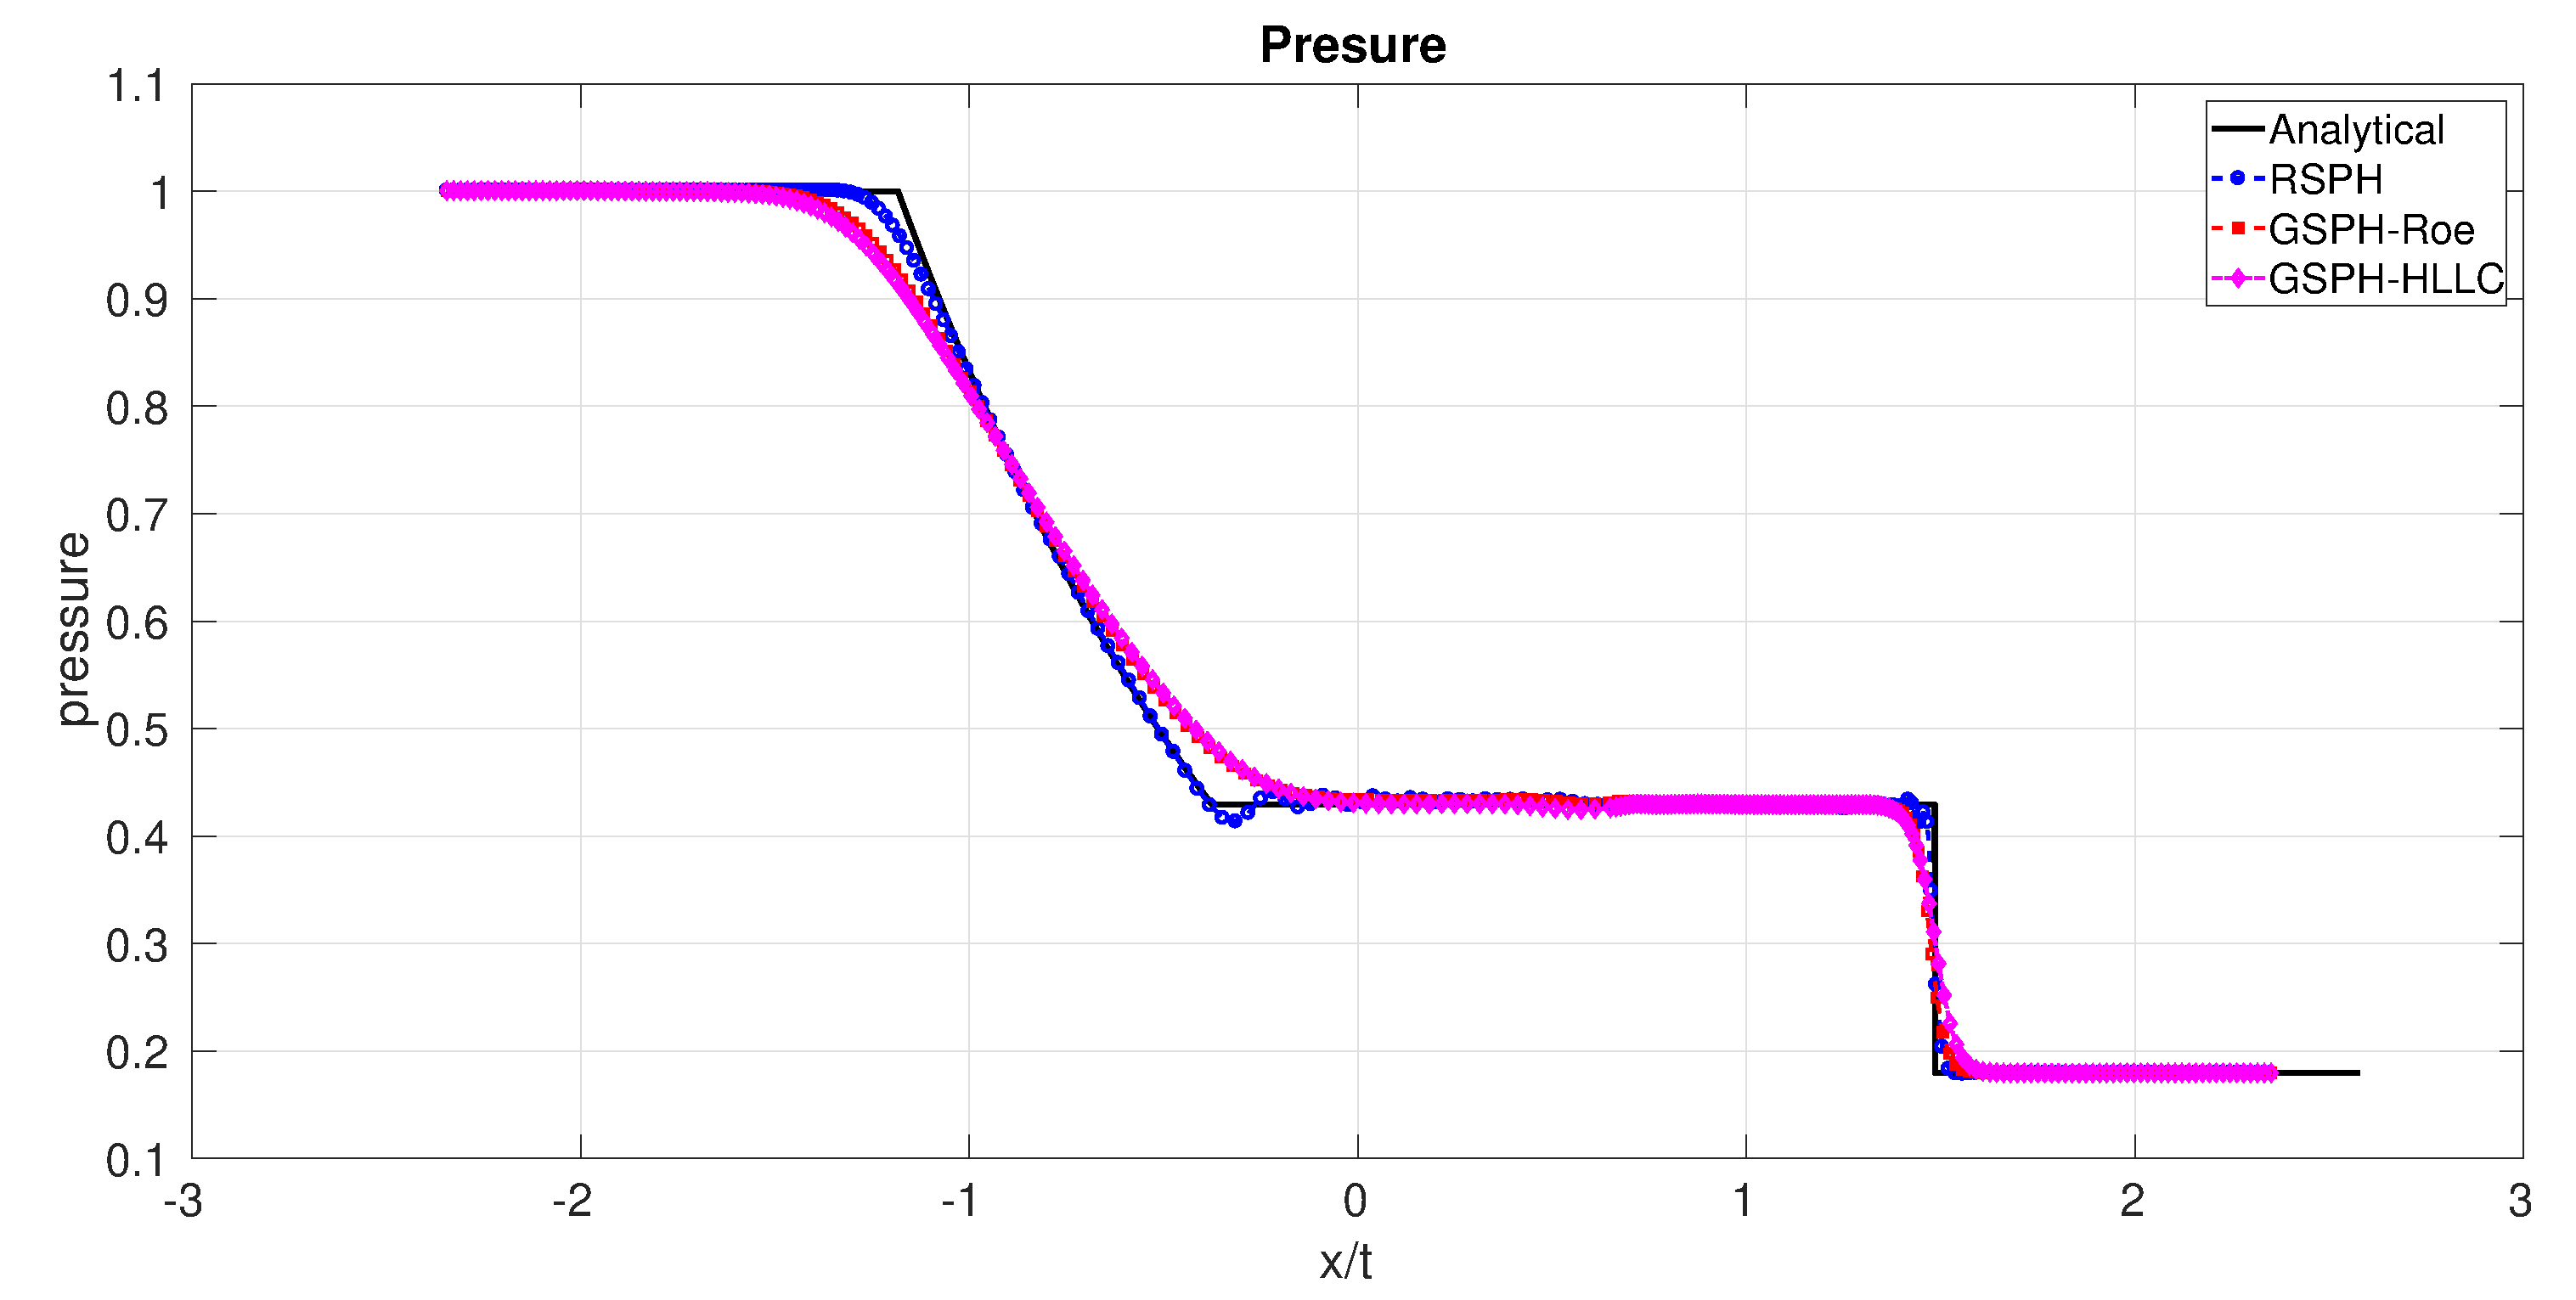
\includegraphics[width=0.99 \textwidth]{./Figures/Sod/RCM-Sod-GSPH-compare-p}
    \end{minipage}% 
    \\
    \begin{minipage}{.495\textwidth}
        \centering
        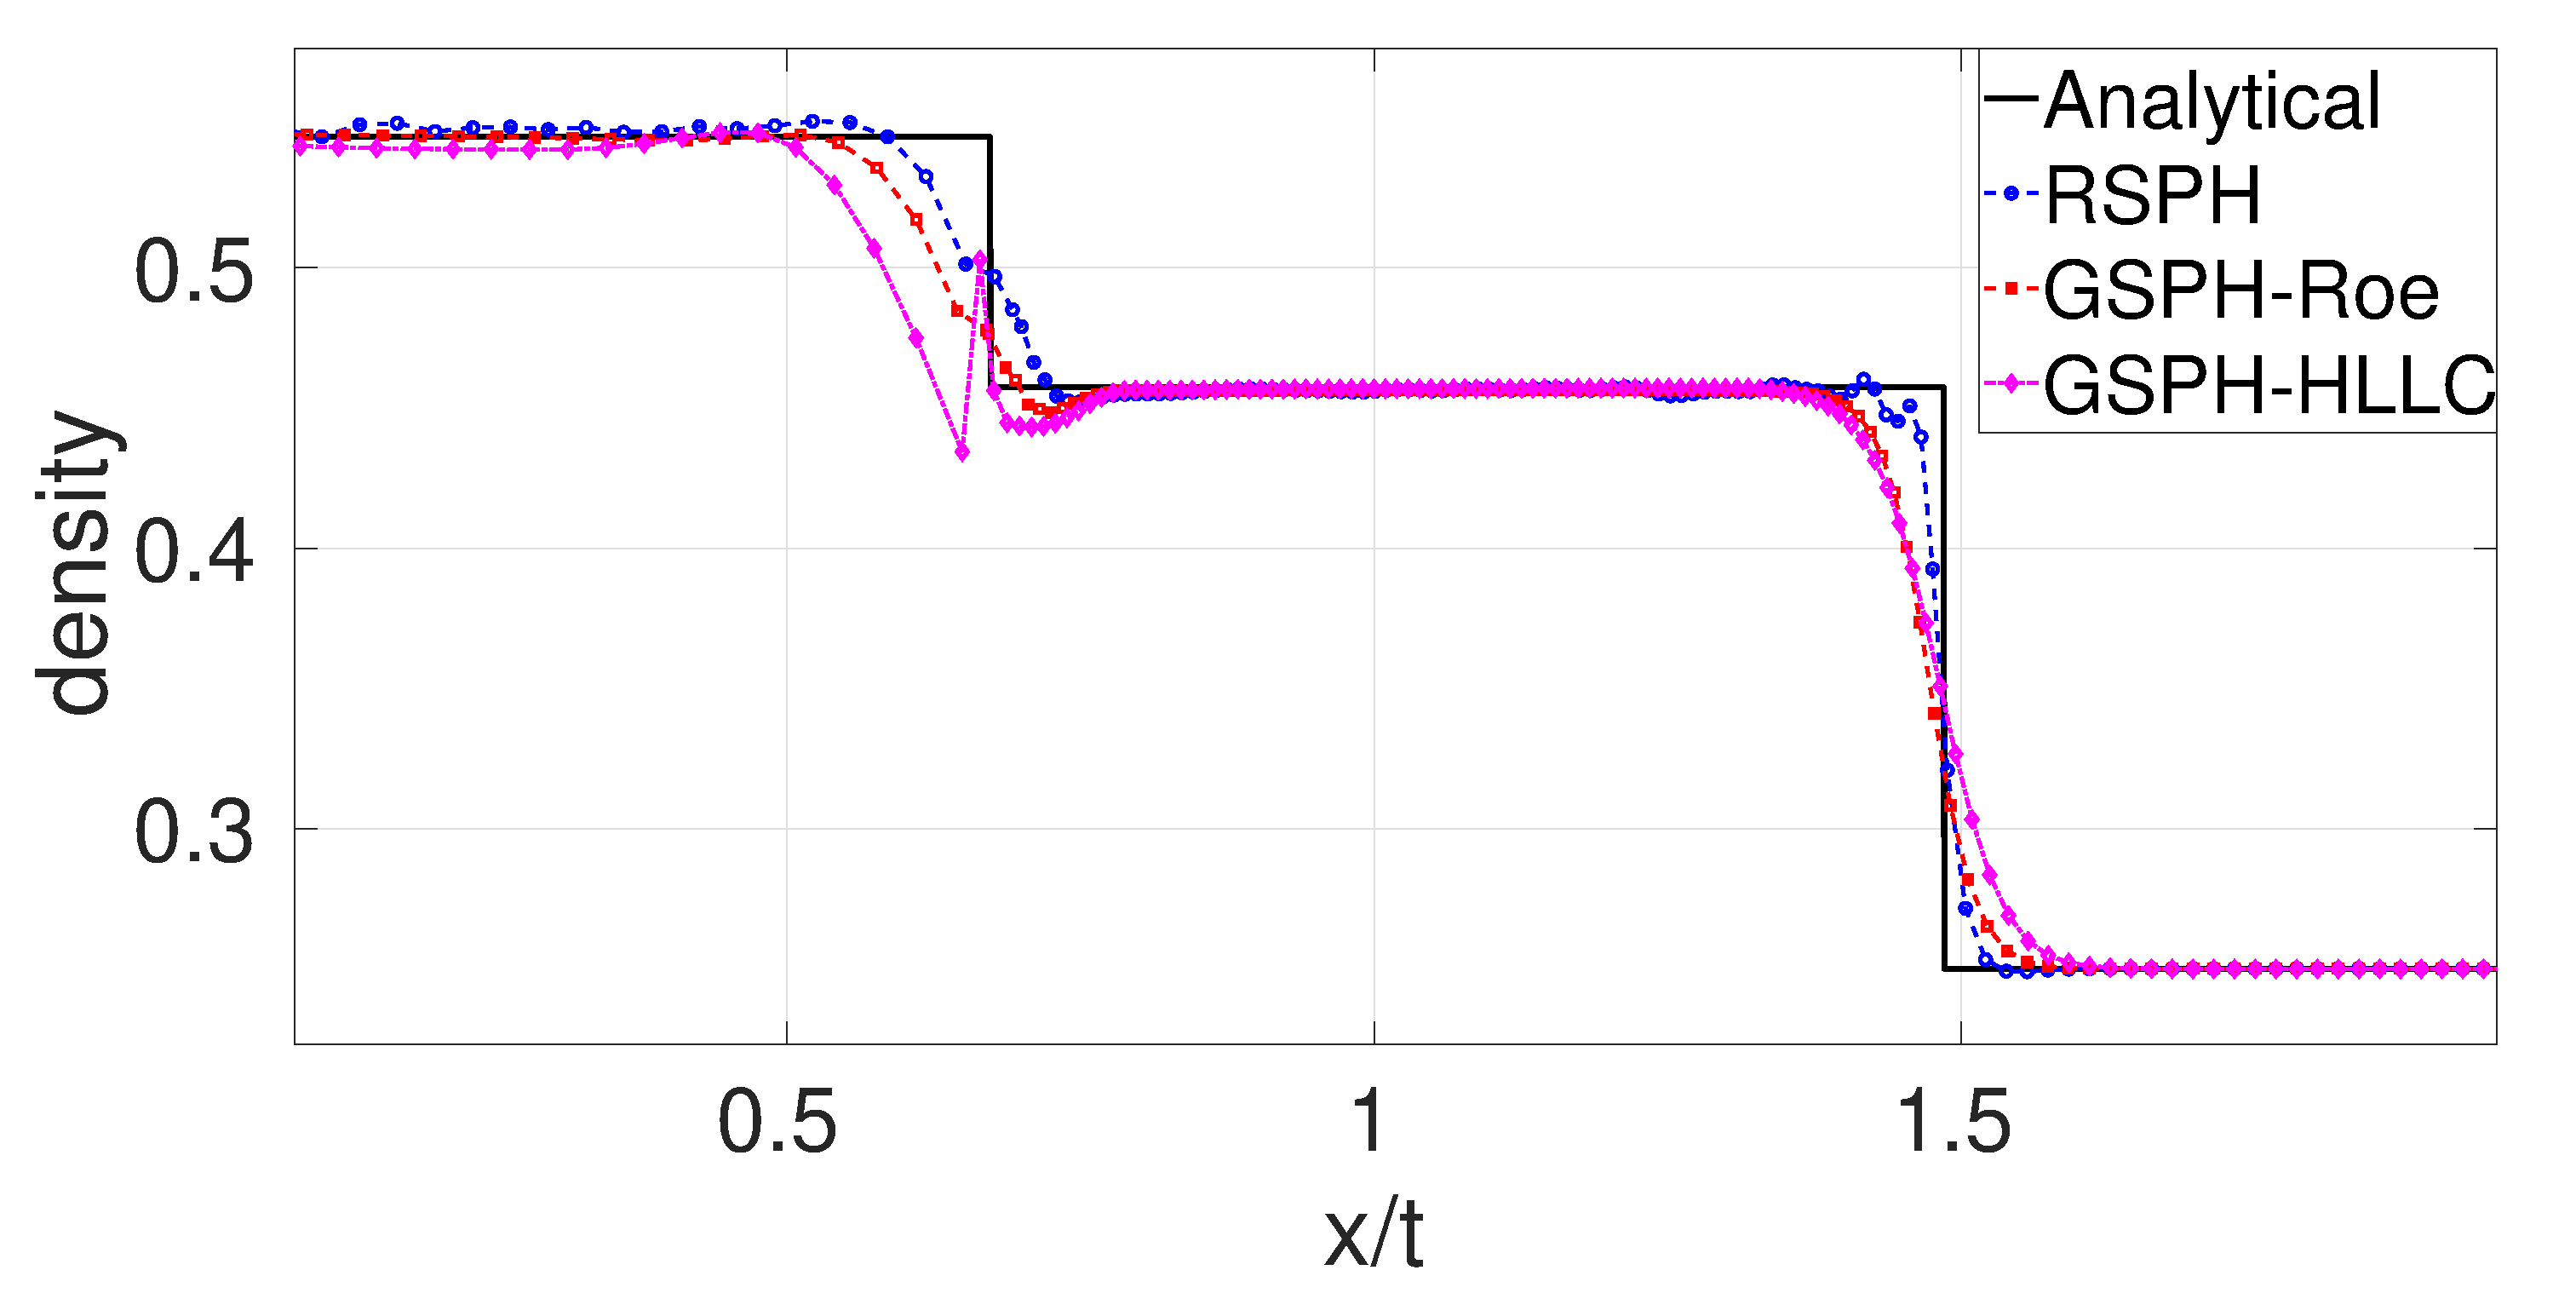
\includegraphics[width=0.99 \textwidth]{./Figures/Sod/RCM-Sod-GSPH-compare-rho-zoom}
    \end{minipage}%
    \begin{minipage}{.495 \textwidth}
        \centering
        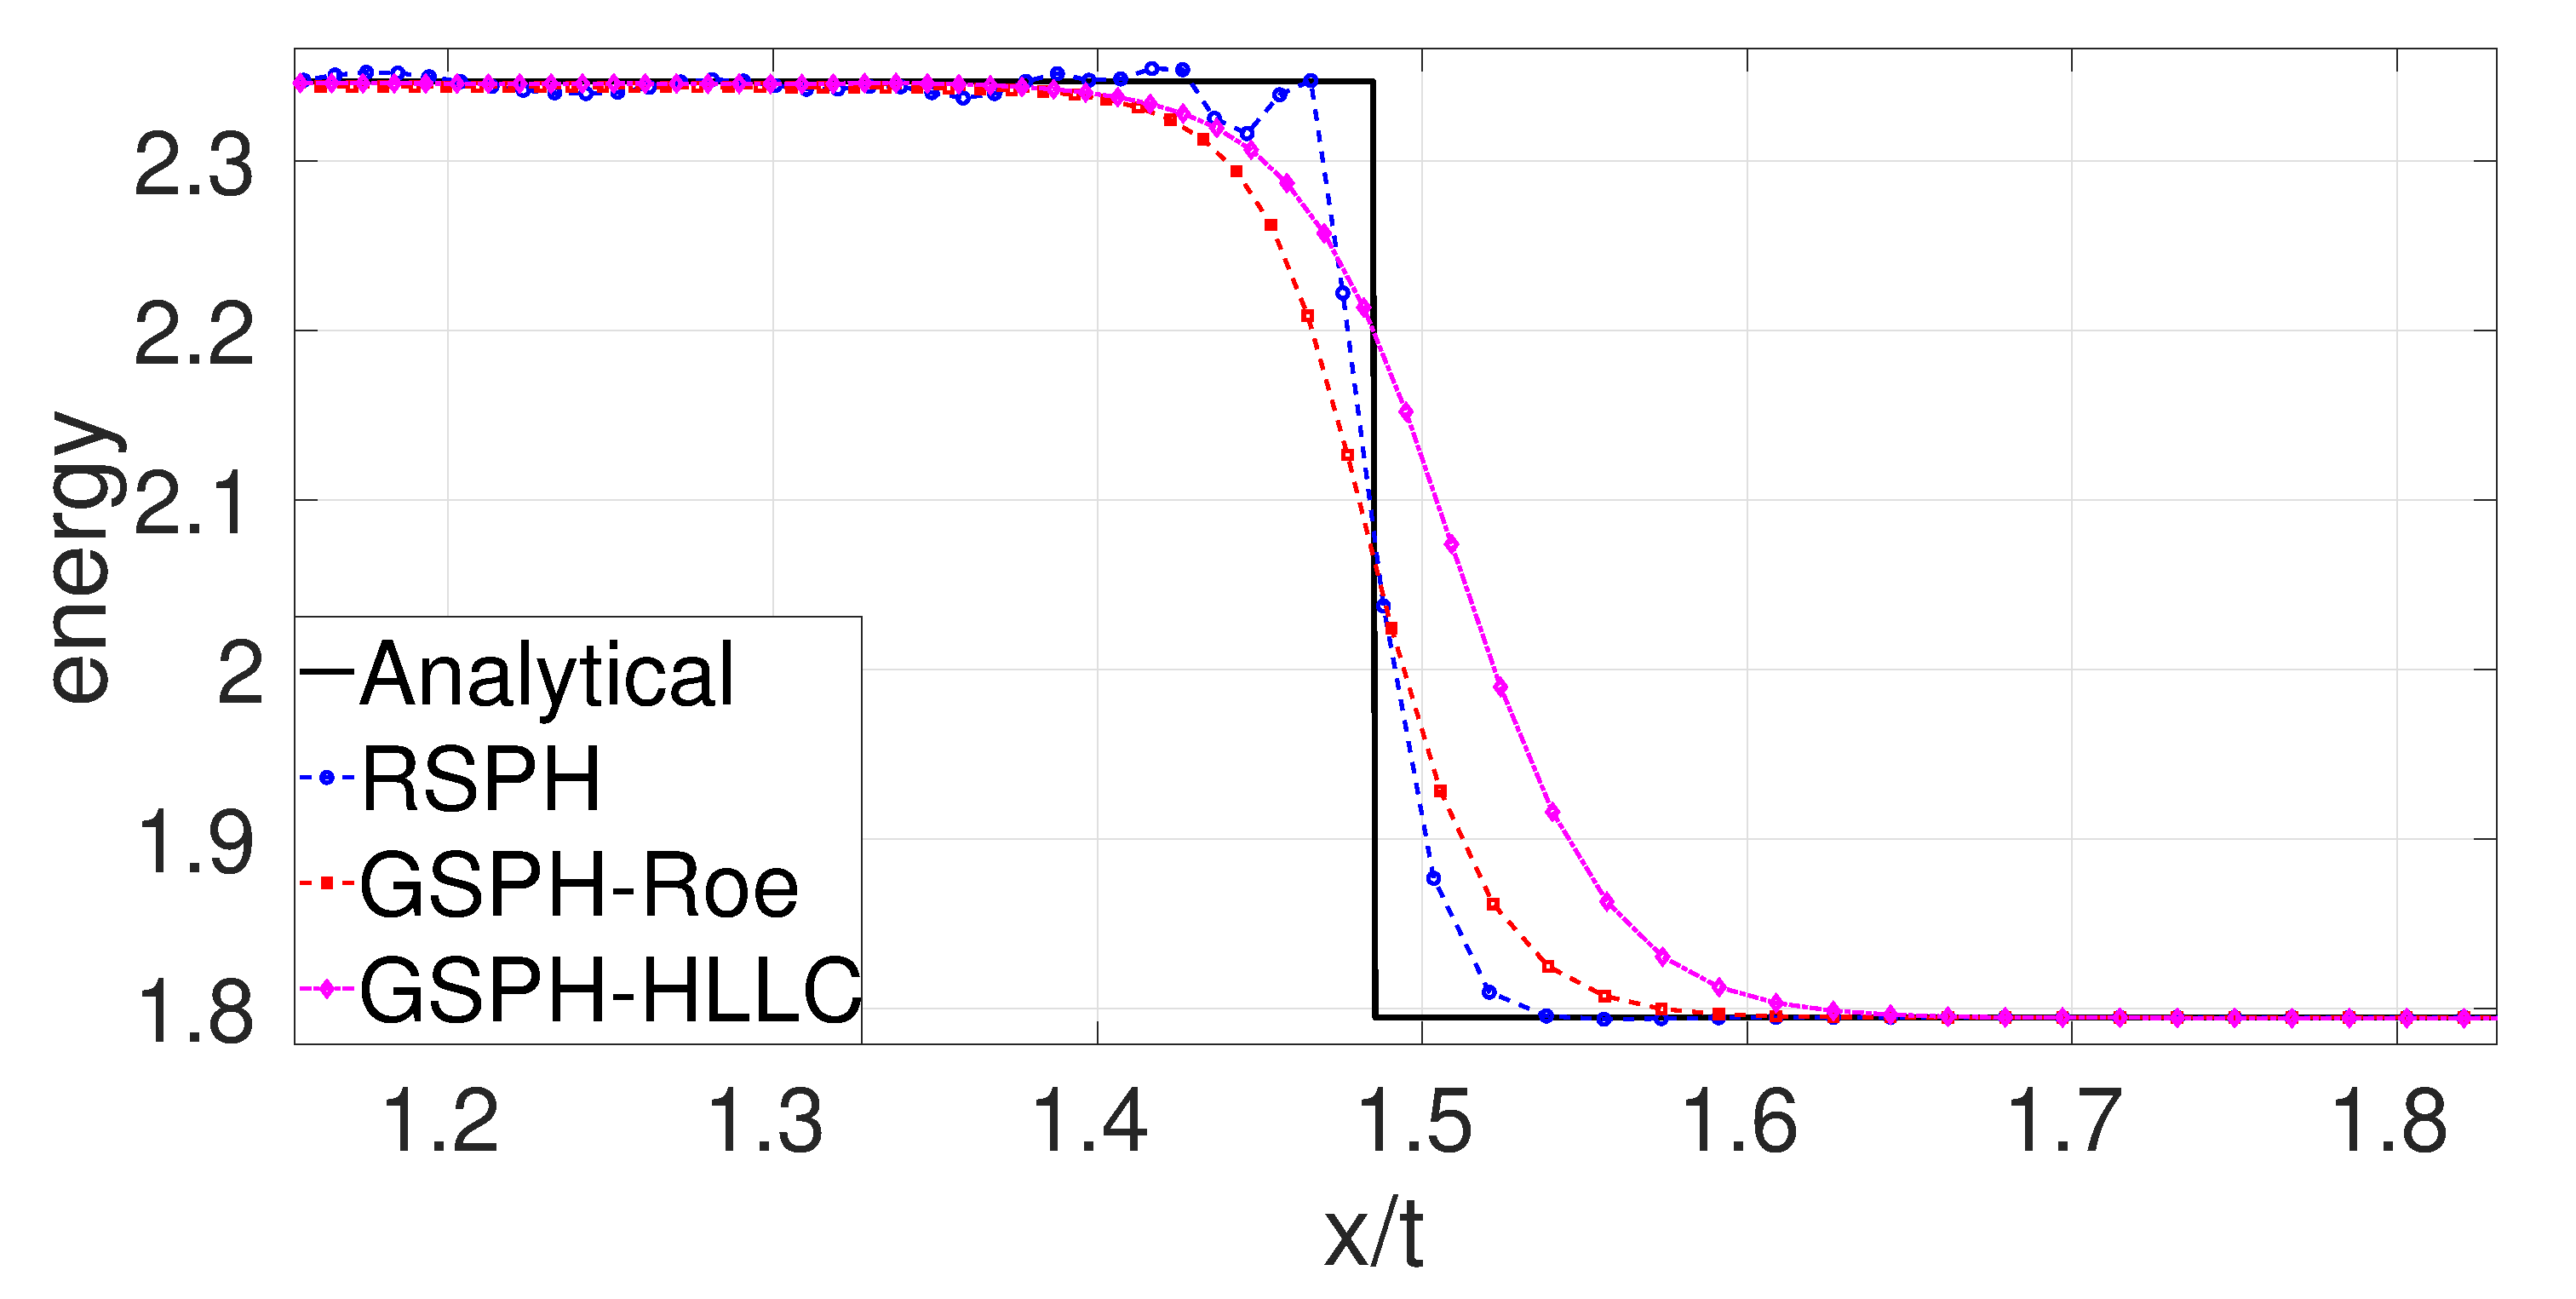
\includegraphics[width=0.99 \textwidth]{./Figures/Sod/RCM-Sod-GSPH-compare-e-zoom}
    \end{minipage}% 
    \\
    \begin{minipage}{.495 \textwidth}
        \centering
        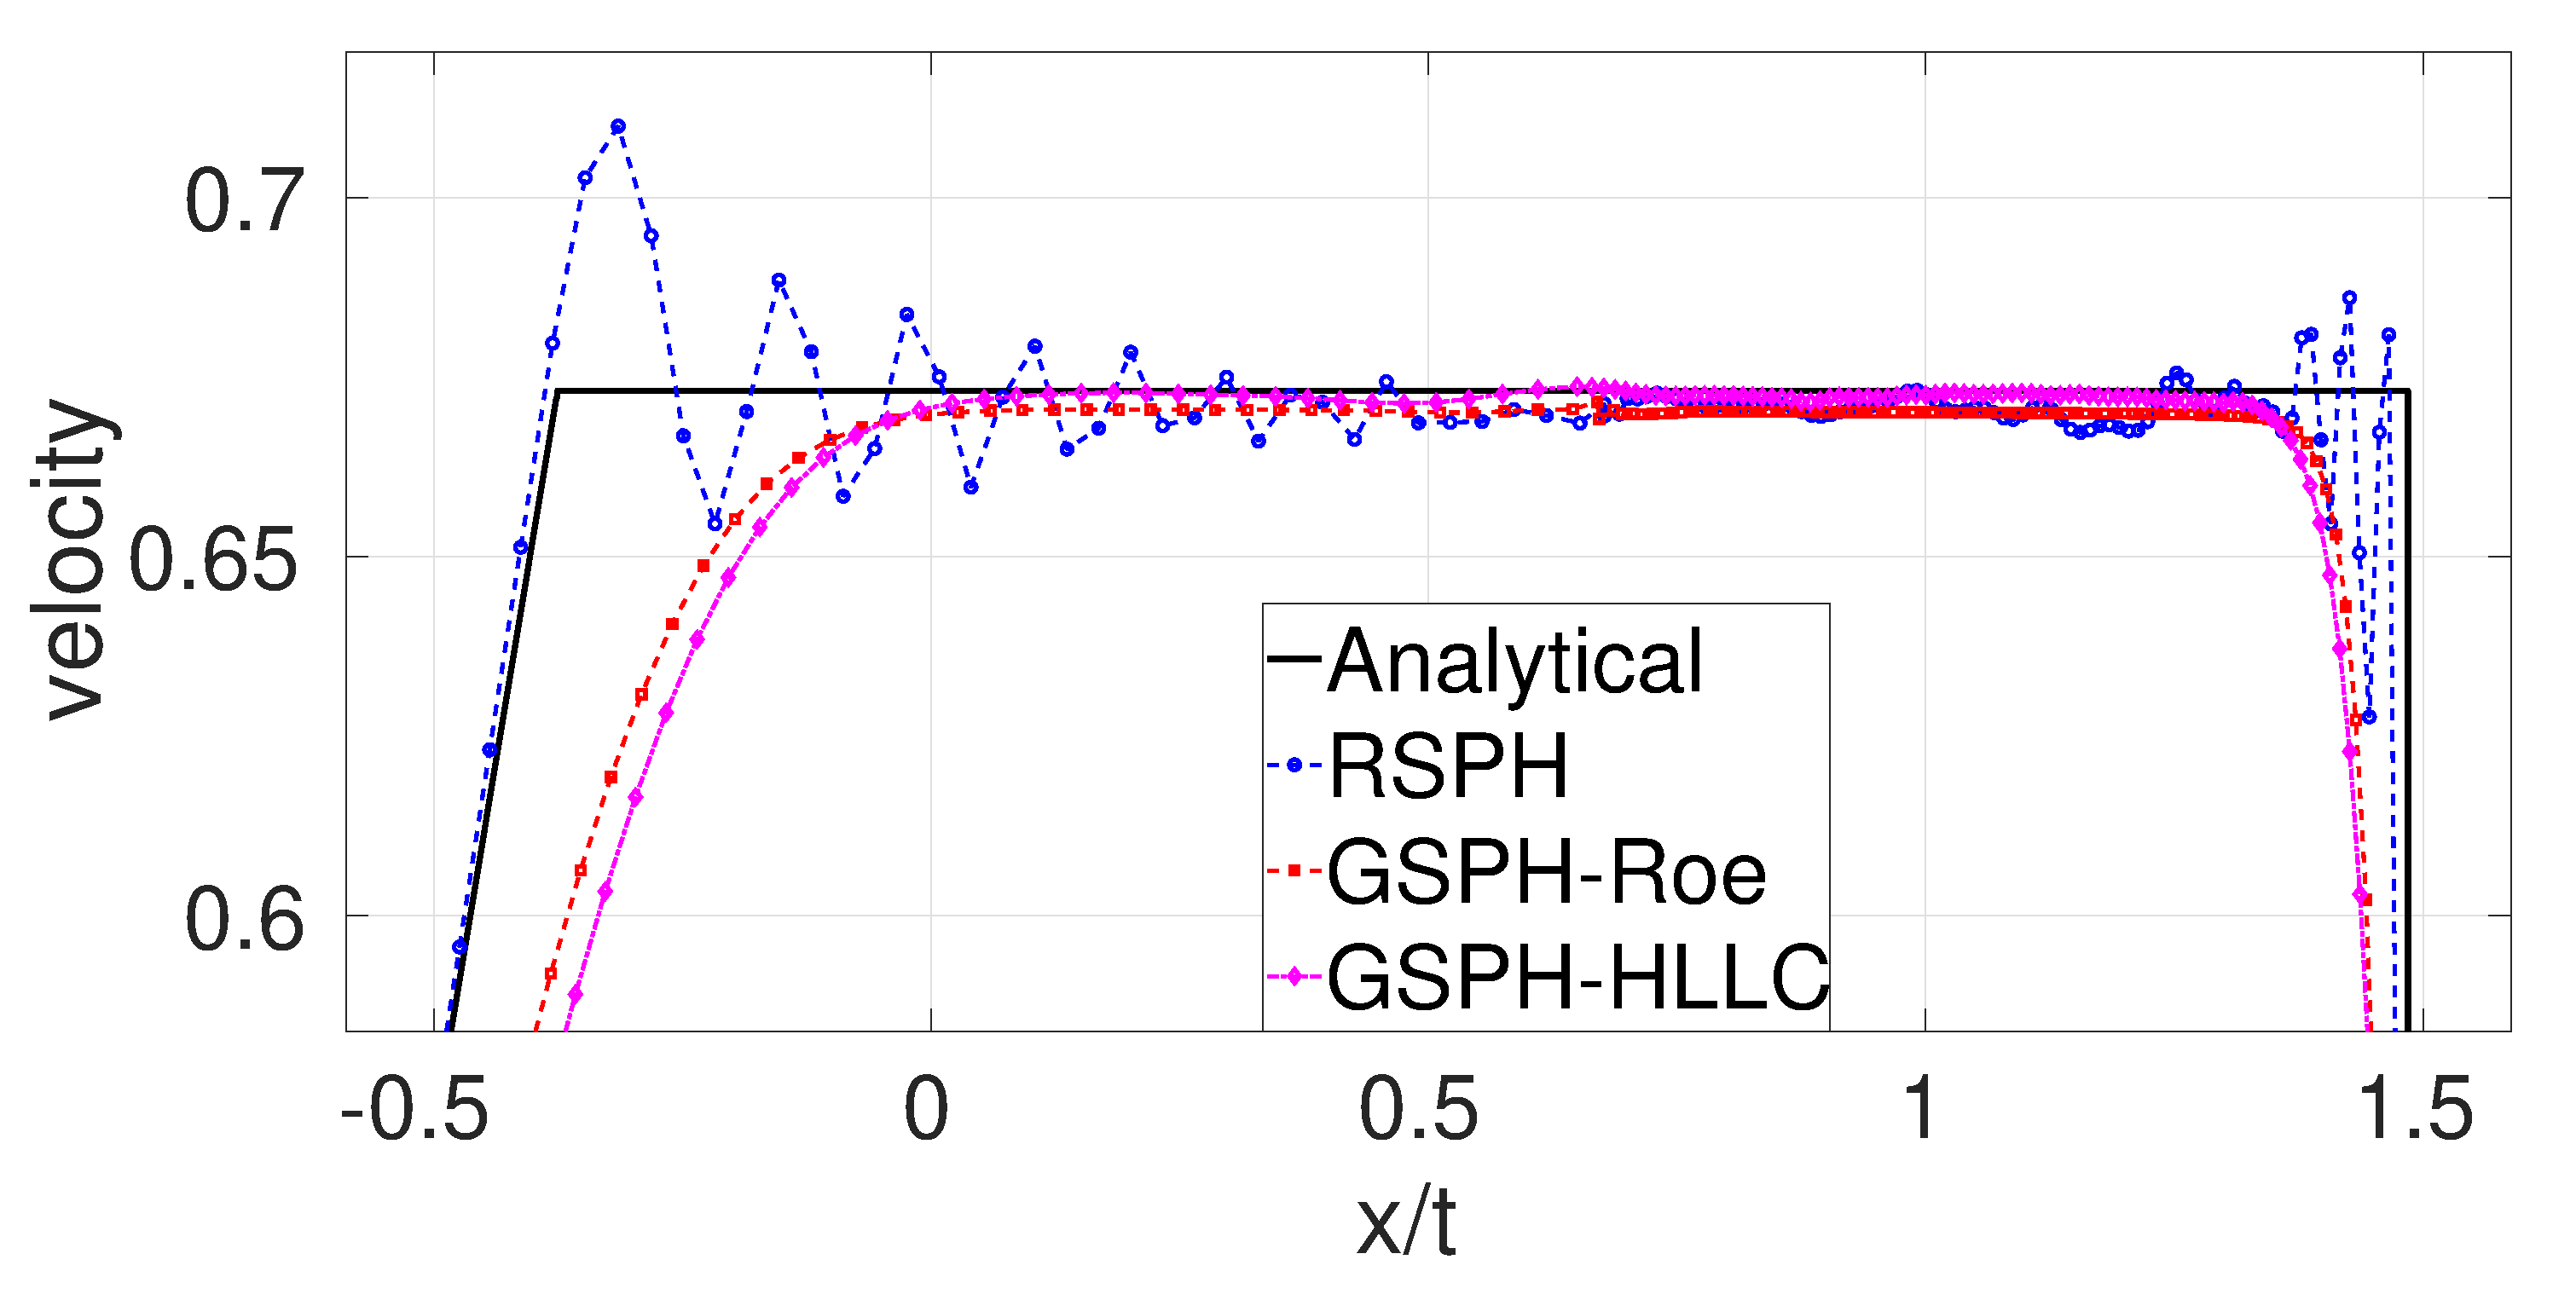
\includegraphics[width=0.99 \textwidth]{./Figures/Sod/RCM-Sod-GSPH-compare-v-zoom}
    \end{minipage}% 
    \begin{minipage}{.495\textwidth}
        \centering
        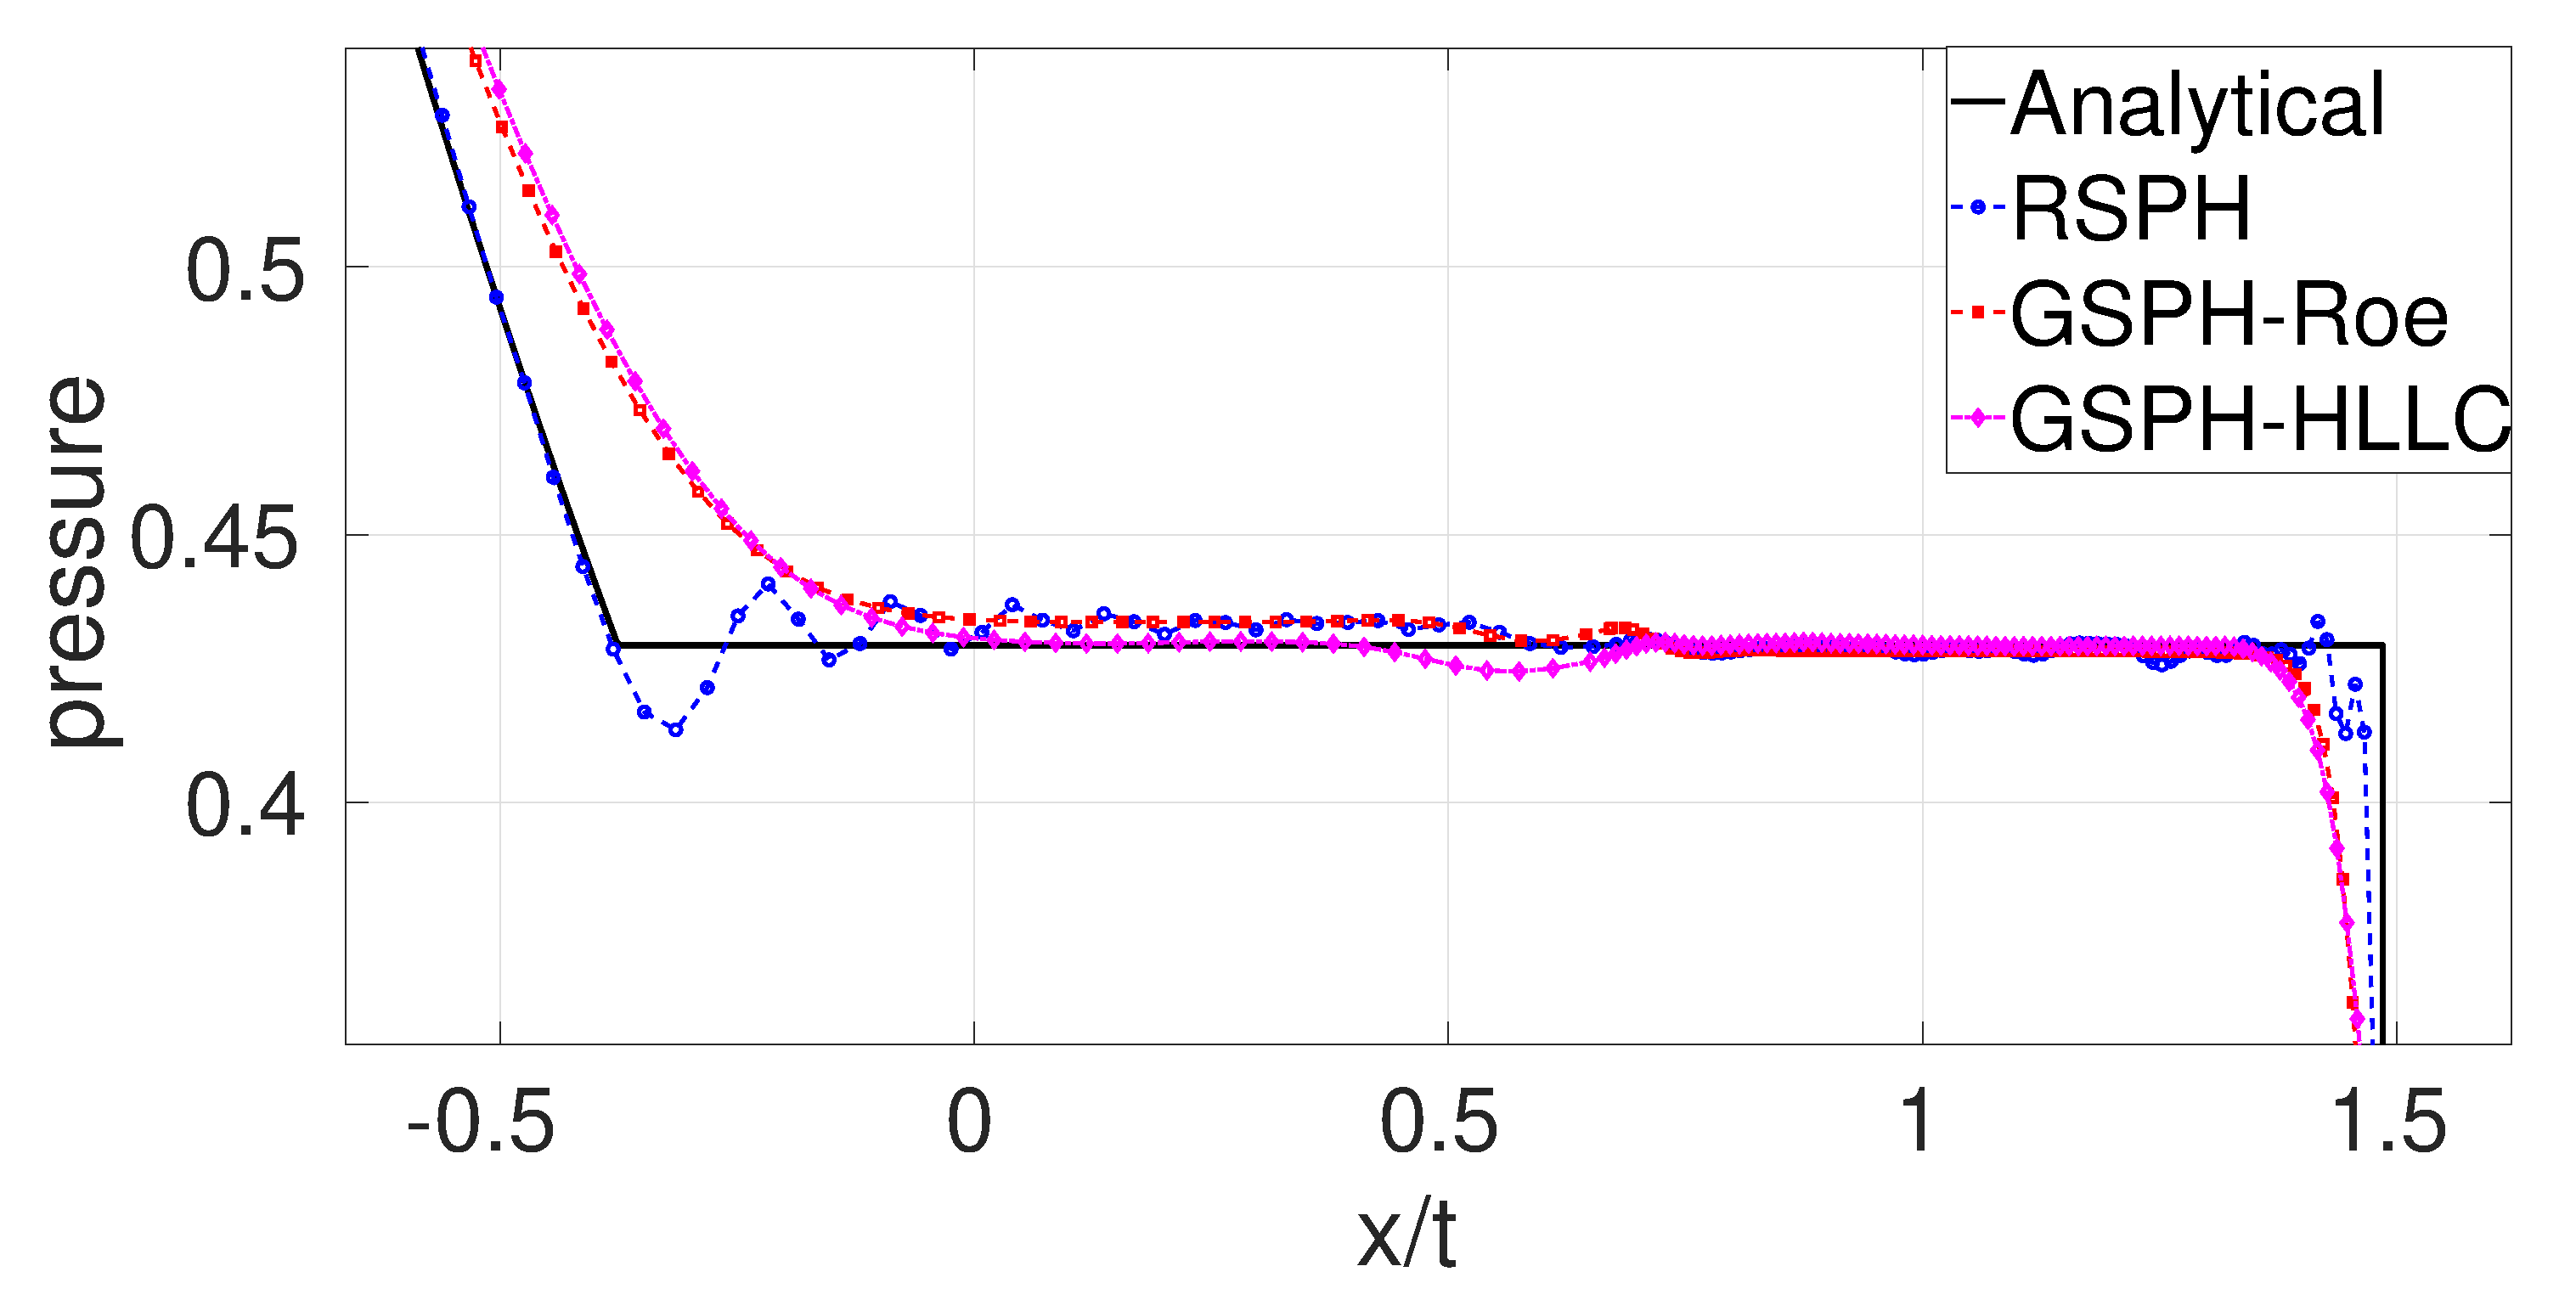
\includegraphics[width=0.99 \textwidth]{./Figures/Sod/RCM-Sod-GSPH-compare-p-zoom}
    \end{minipage}%    
    \caption{Comparison of RSPH with GSPH using Roe Riemann solver and HLLC Riemann solver. The last four plots are zoomed views. Zoomed view of density and specific internal energy show that GSPH smears the discontinuity at shock much more than RSPH. Zoomed view of velocity shows that fluctuation in GSPH is completely suppressed, which implies that numerical dissipation introduced in GSPH is at least around the same amount as SPH with $\alpha=1.0$. This is consisitent with information implied by zoomed view of density and specific internal energy. The last zoomed view shows that both RSPH and GSPH can get rid of pressure "wiggle" around the contact discontinuity.}
    \label{fig:RCM-Sod-GSPH}
\end{figure}

These zoomed views in fig. \ref{fig:RCM-Sod-GSPH} demonstrate that RSPH introduces less but sufficient dissipation compared with GSPH. The attractive feature of RCM method in preserving true discontinuity is inherited by RSPH in this 1D shock tube test. With more dissipation, GSPH can completely suppress numerical dissipation, the discontinuity at the shock is more seriously smeared. The excessive amount dissipation might have other, more undesirable, affect in real implementation. Such undesirable effect will be shown in next section. Compared with SPH, both GSPH and RSPH avoid pressure "wiggles" around contact discontinuity. 

\subsection{Accuracy tests}

\subsection{Comprehensive tests}
Comprehensive tests are presented in this section to check how well does RSPH work for different situations. Input parameters for each tests is given in Table \ref{tab:1D-shock-input_parameters}. Wave speed is estimated based on formulation Eq. (\ref{eq:RP-solver-HLLC-SM}) $\sim$ Eq. (\ref{eq:RP-solver-HLLC-SR})
The results are shown in figures below. Current scheme is able to correctly predict the position and magnitude of all waves for all tests. Due to less amount of dissipation, fluctuations do not decay completely in RSPH. For the the strong blast test and double shock test, such fluctuation becomes pretty obvious.

\begin{figure}[H]
    \centering
    \begin{minipage}{.245\textwidth}
        \centering
        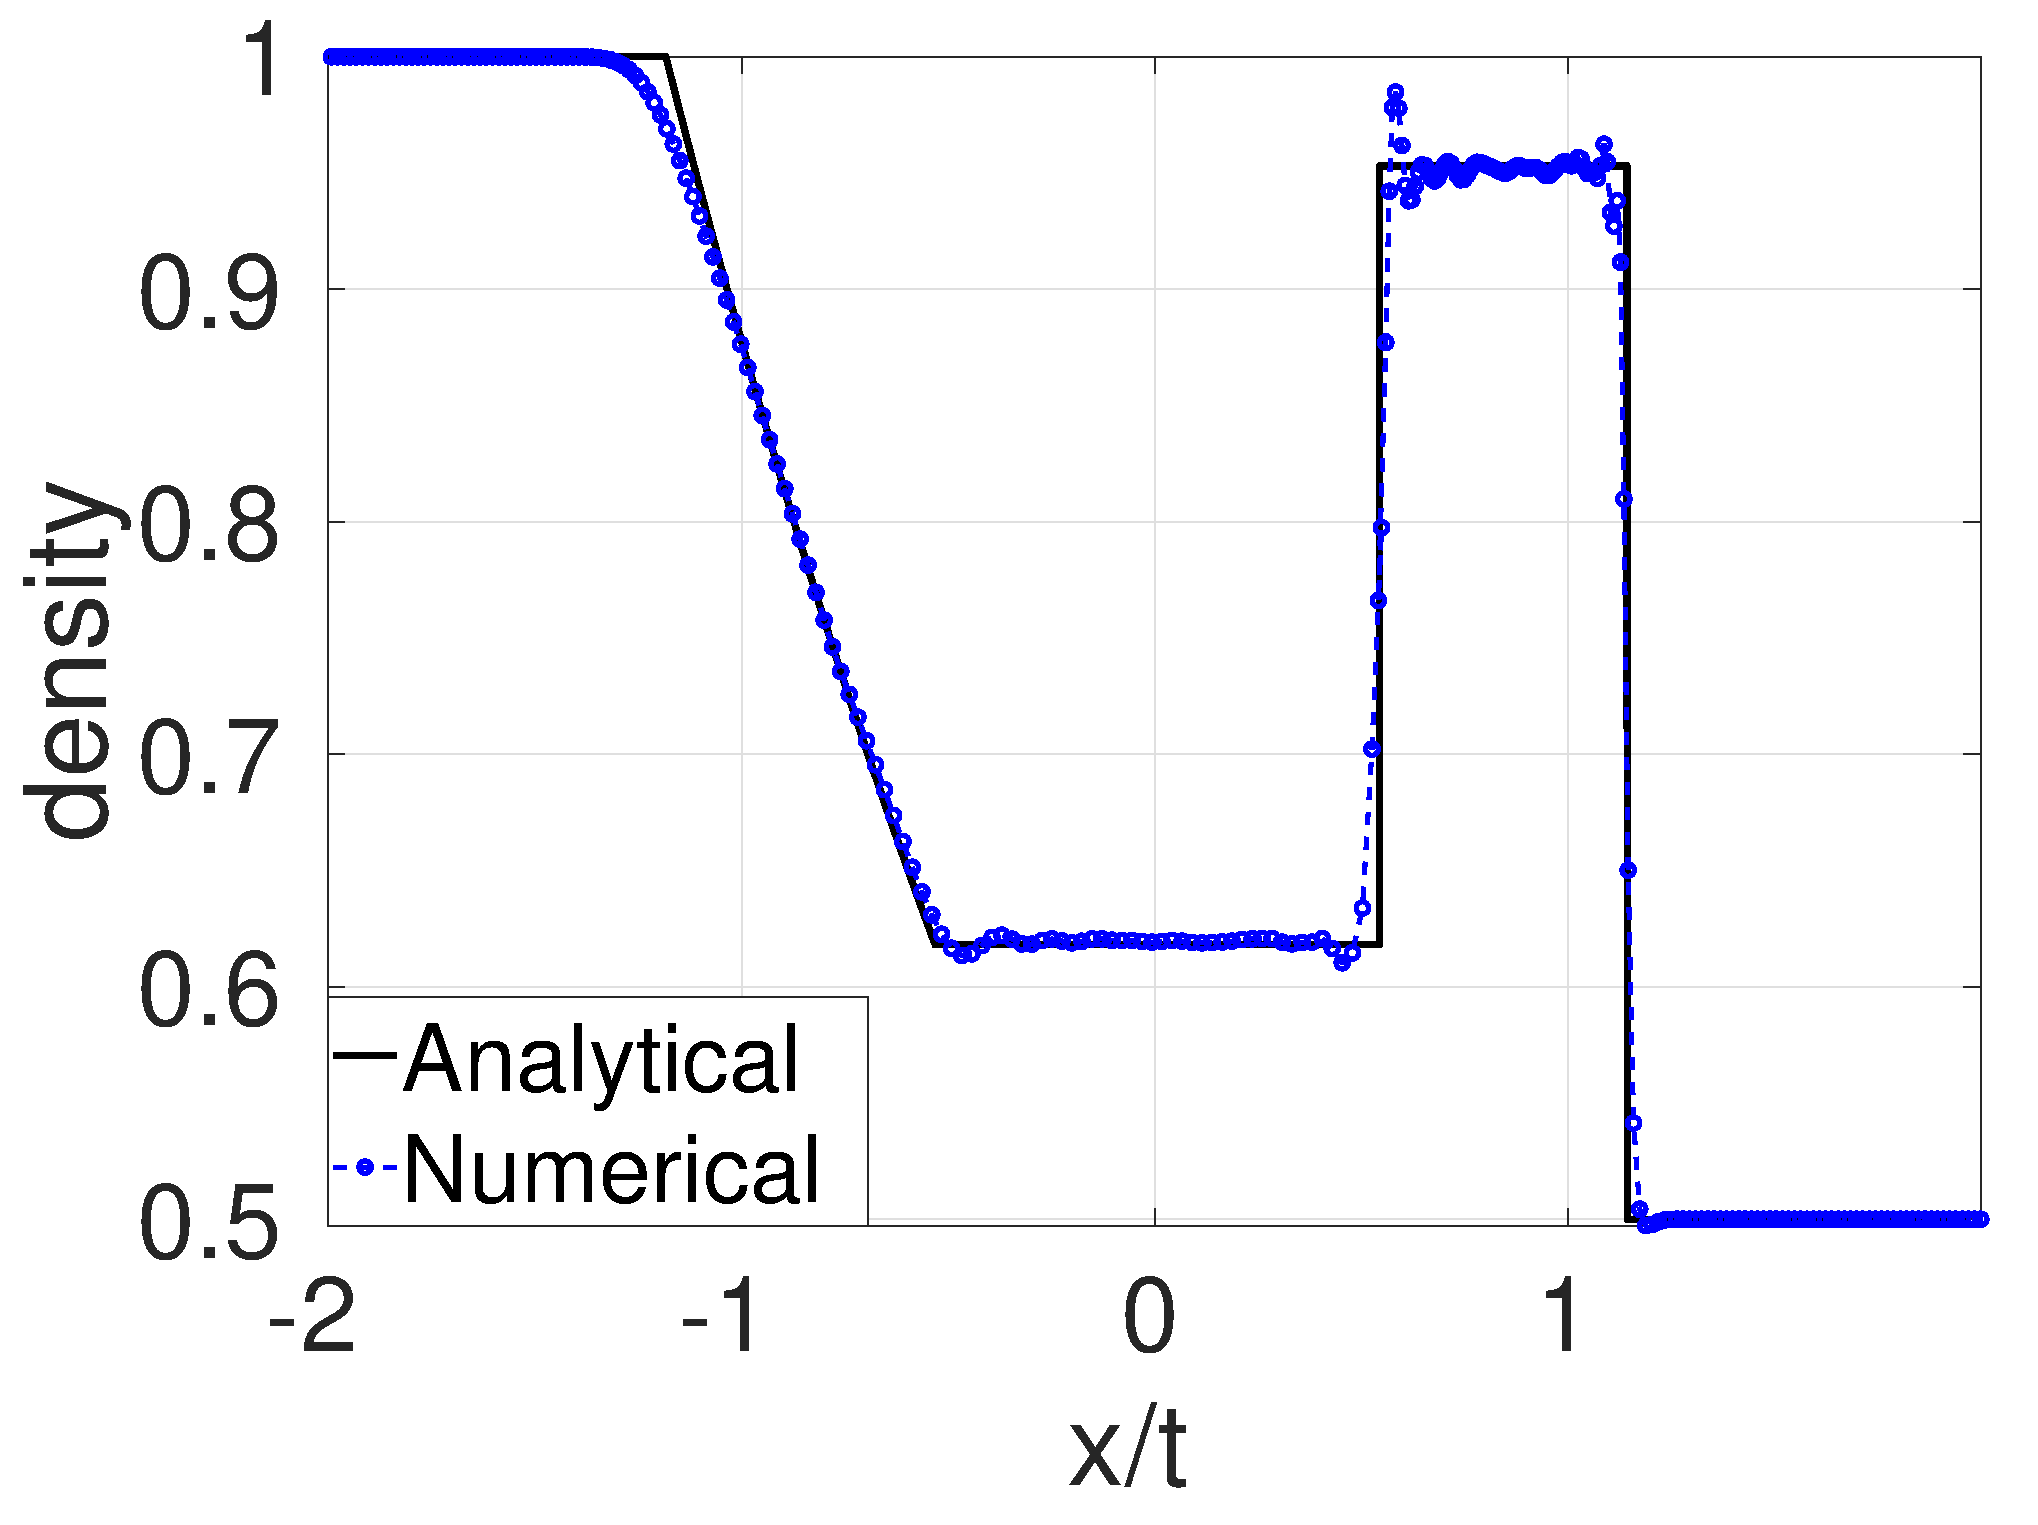
\includegraphics[width=0.99 \textwidth]{./Figures/GSPH-Sod/GRod-RCM-rho}
    \end{minipage}%
    \begin{minipage}{.245 \textwidth}
        \centering
        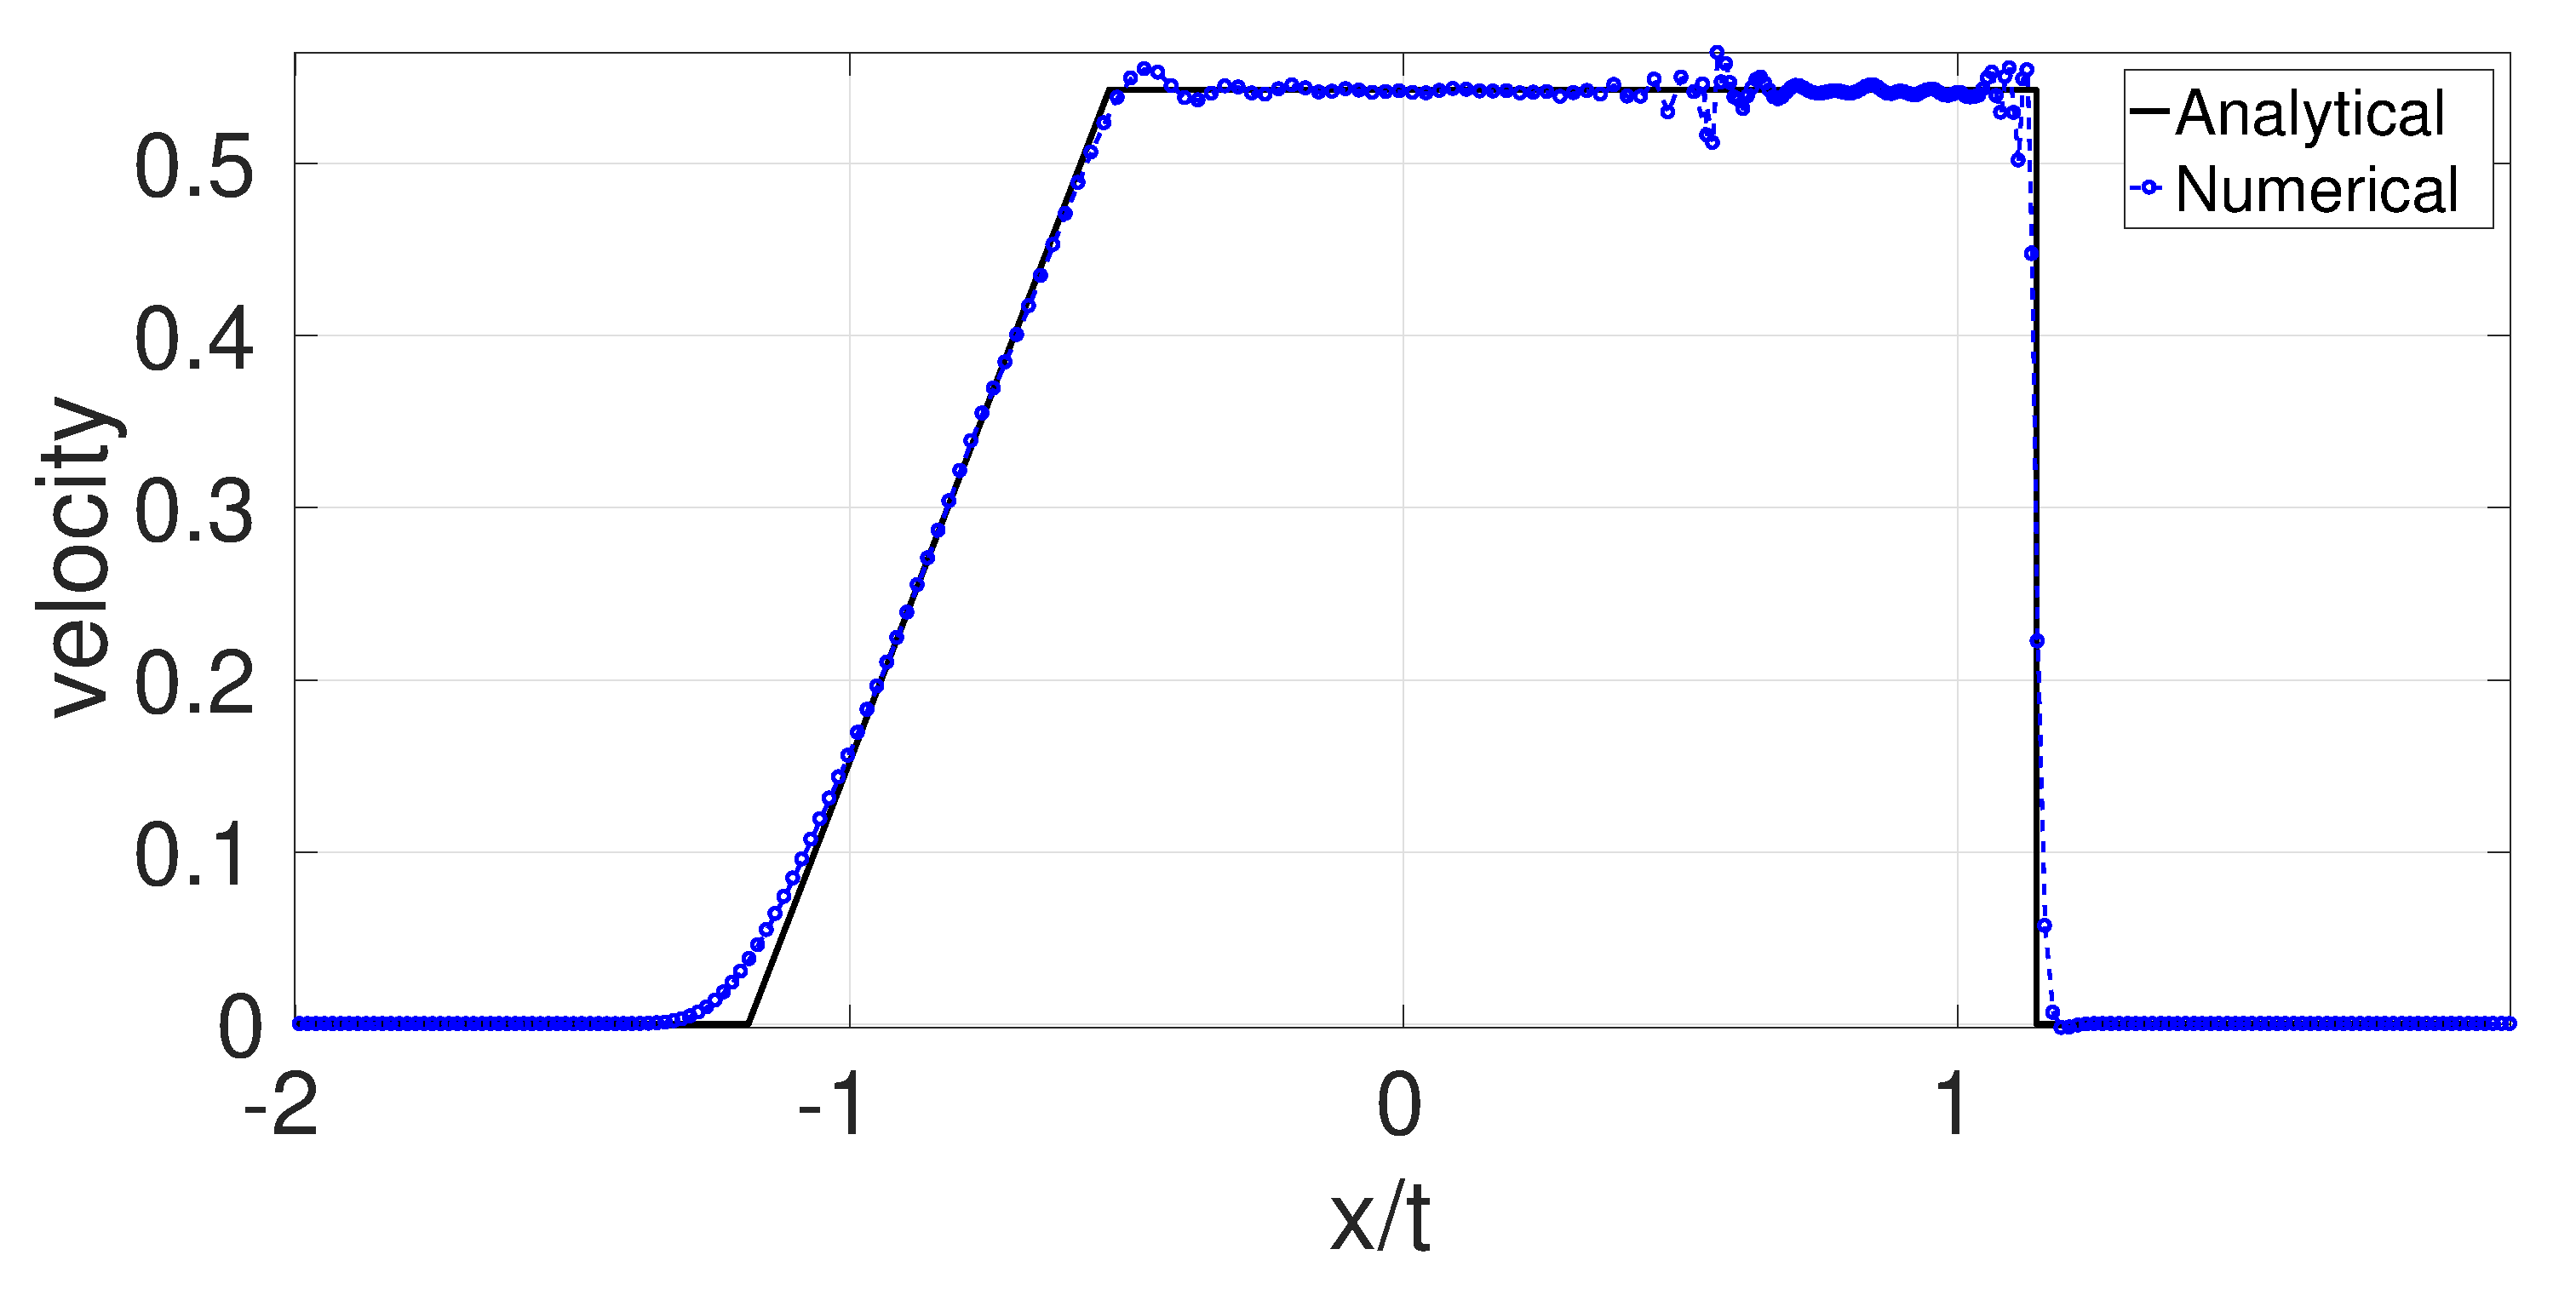
\includegraphics[width=0.99 \textwidth]{./Figures/GSPH-Sod/GRod-RCM-v}
    \end{minipage}%
    \begin{minipage}{.245\textwidth}
        \centering
        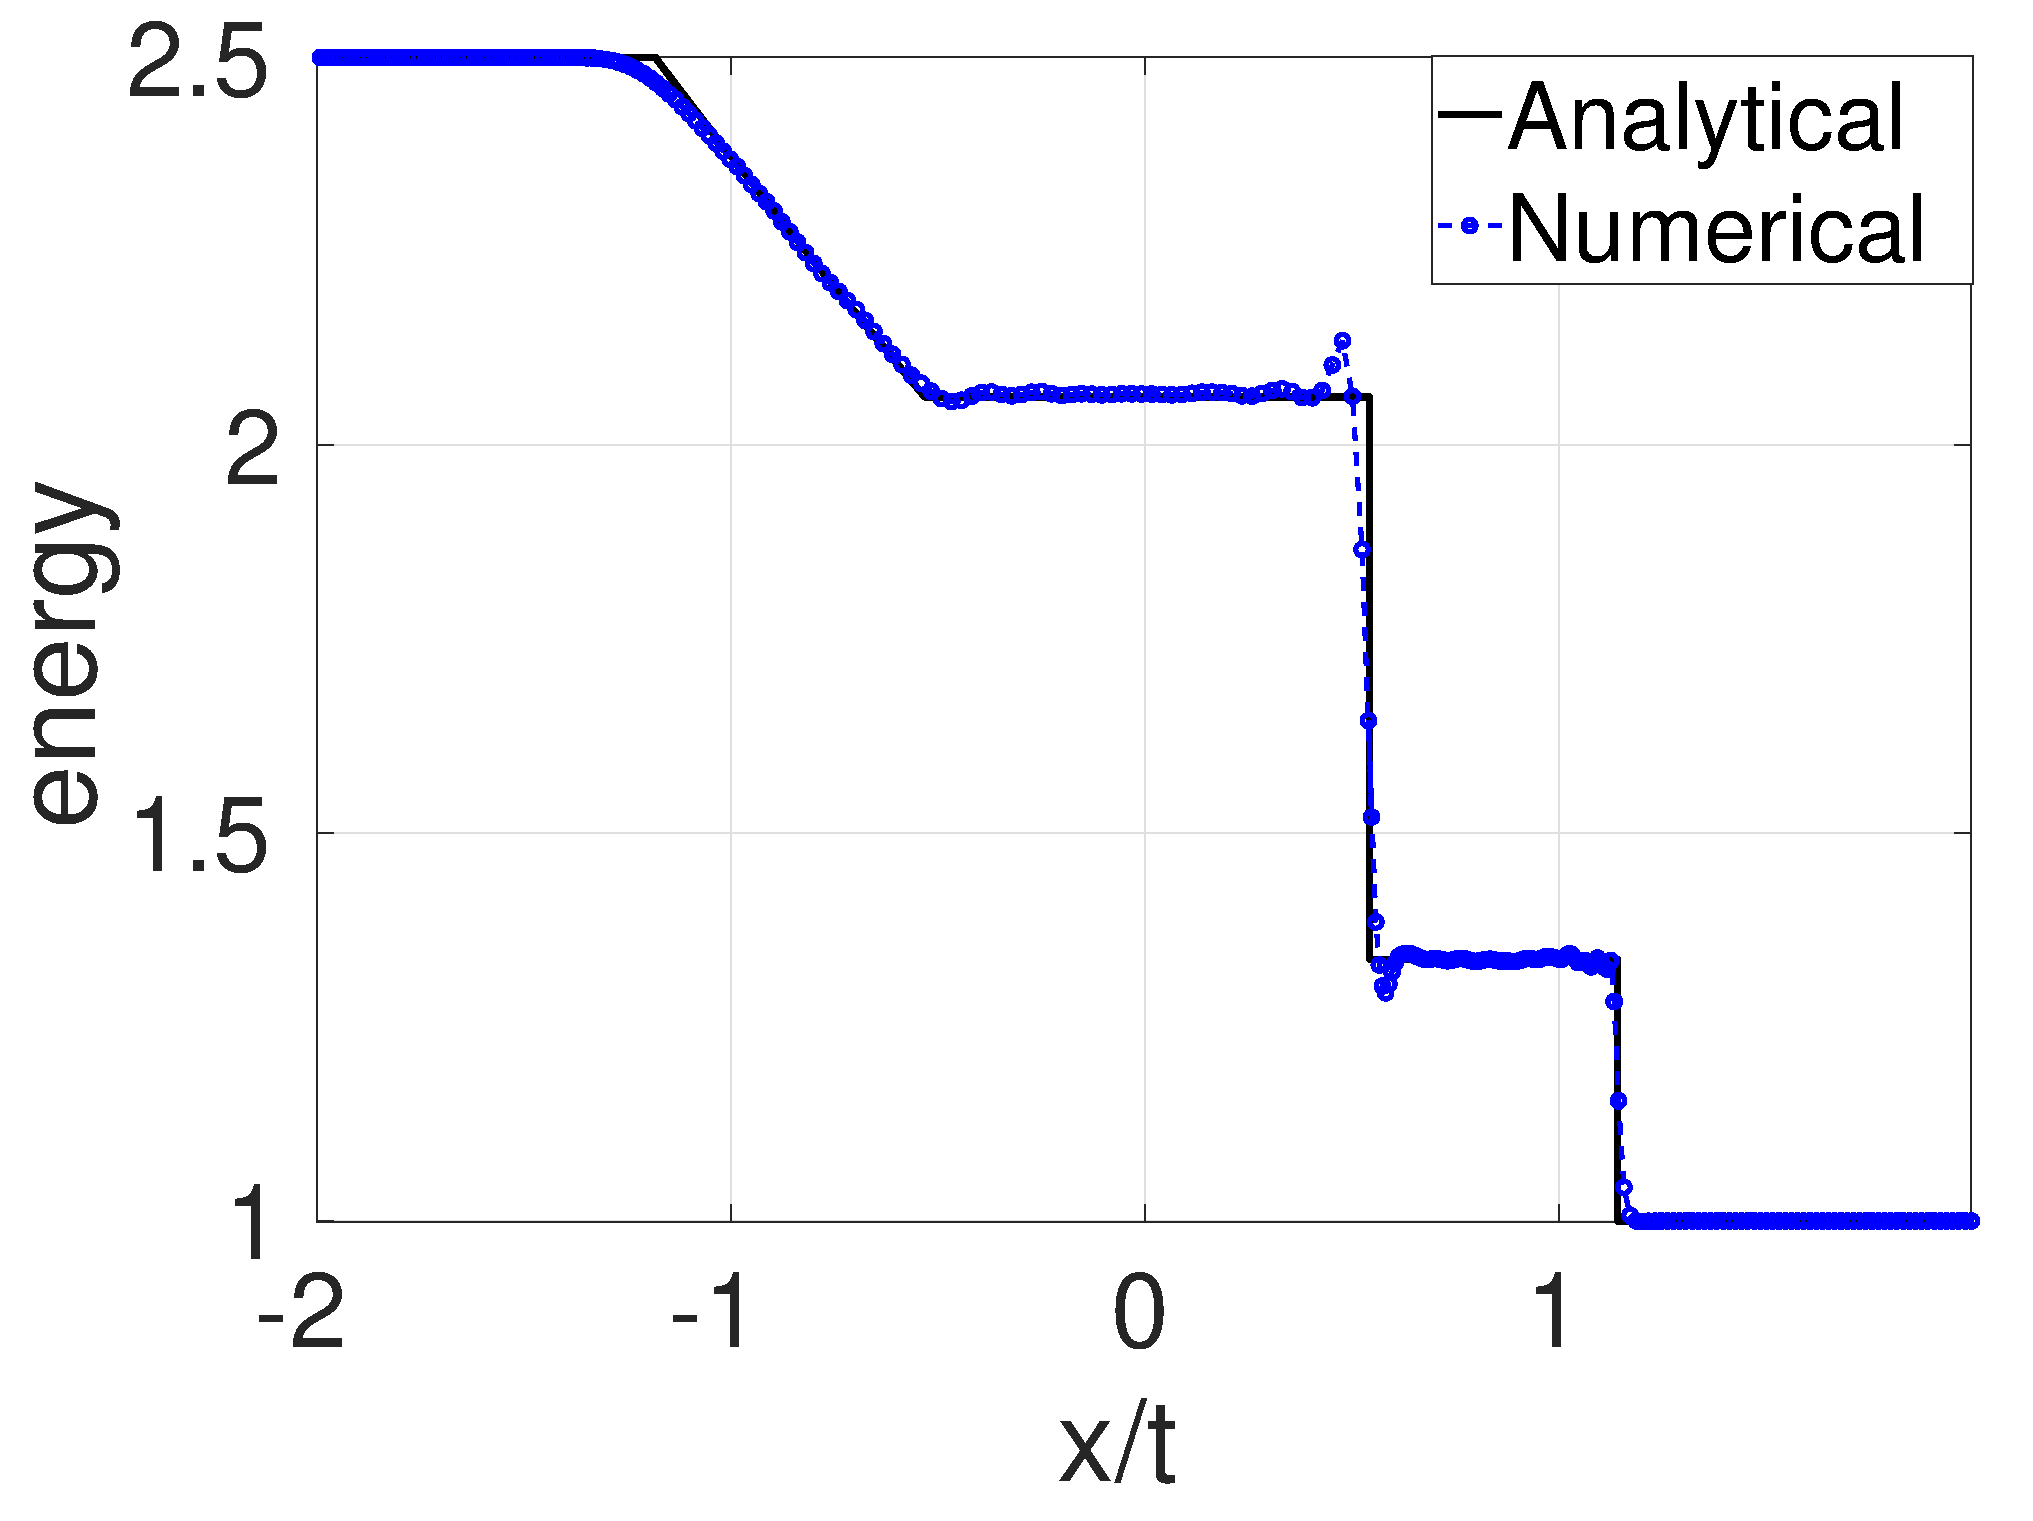
\includegraphics[width=0.99 \textwidth]{./Figures/GSPH-Sod/GRod-RCM-e}
    \end{minipage}%
    \begin{minipage}{.245 \textwidth}
        \centering
        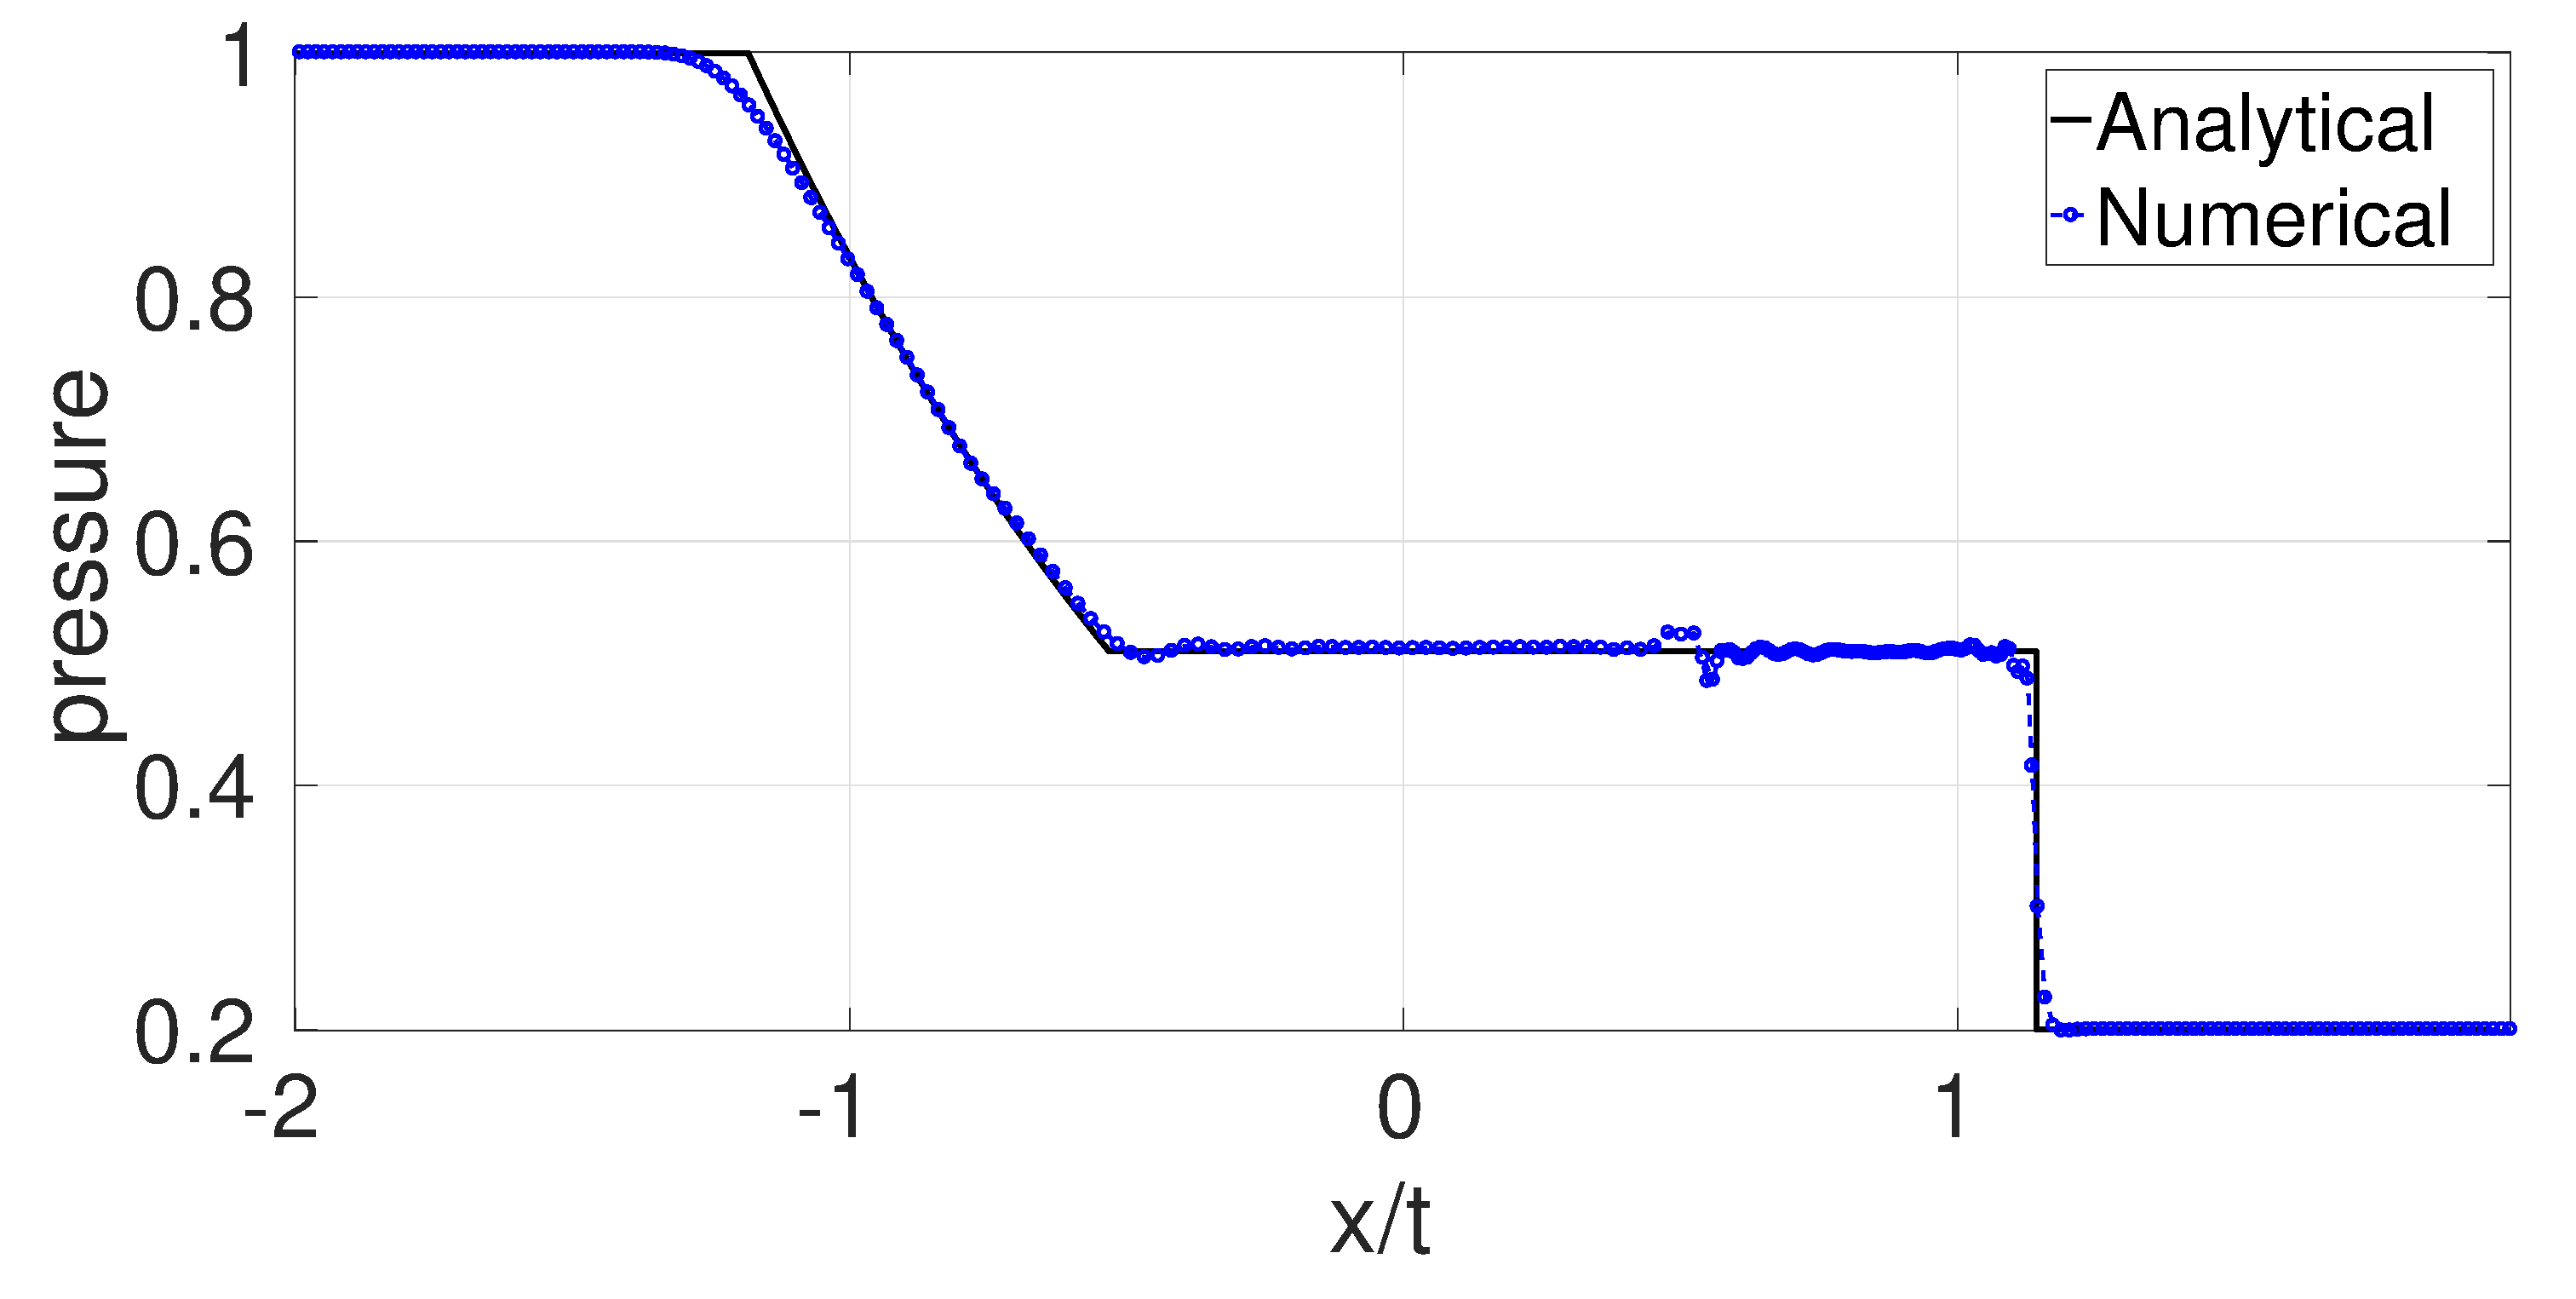
\includegraphics[width=0.99 \textwidth]{./Figures/GSPH-Sod/GRod-RCM-p}
    \end{minipage}% 
    \caption{Results for test 1.}
    \label{fig:RCM-GSPH-Sod}
\end{figure}
\begin{figure}[H]
    \centering
    \begin{minipage}{.245\textwidth}
        \centering
        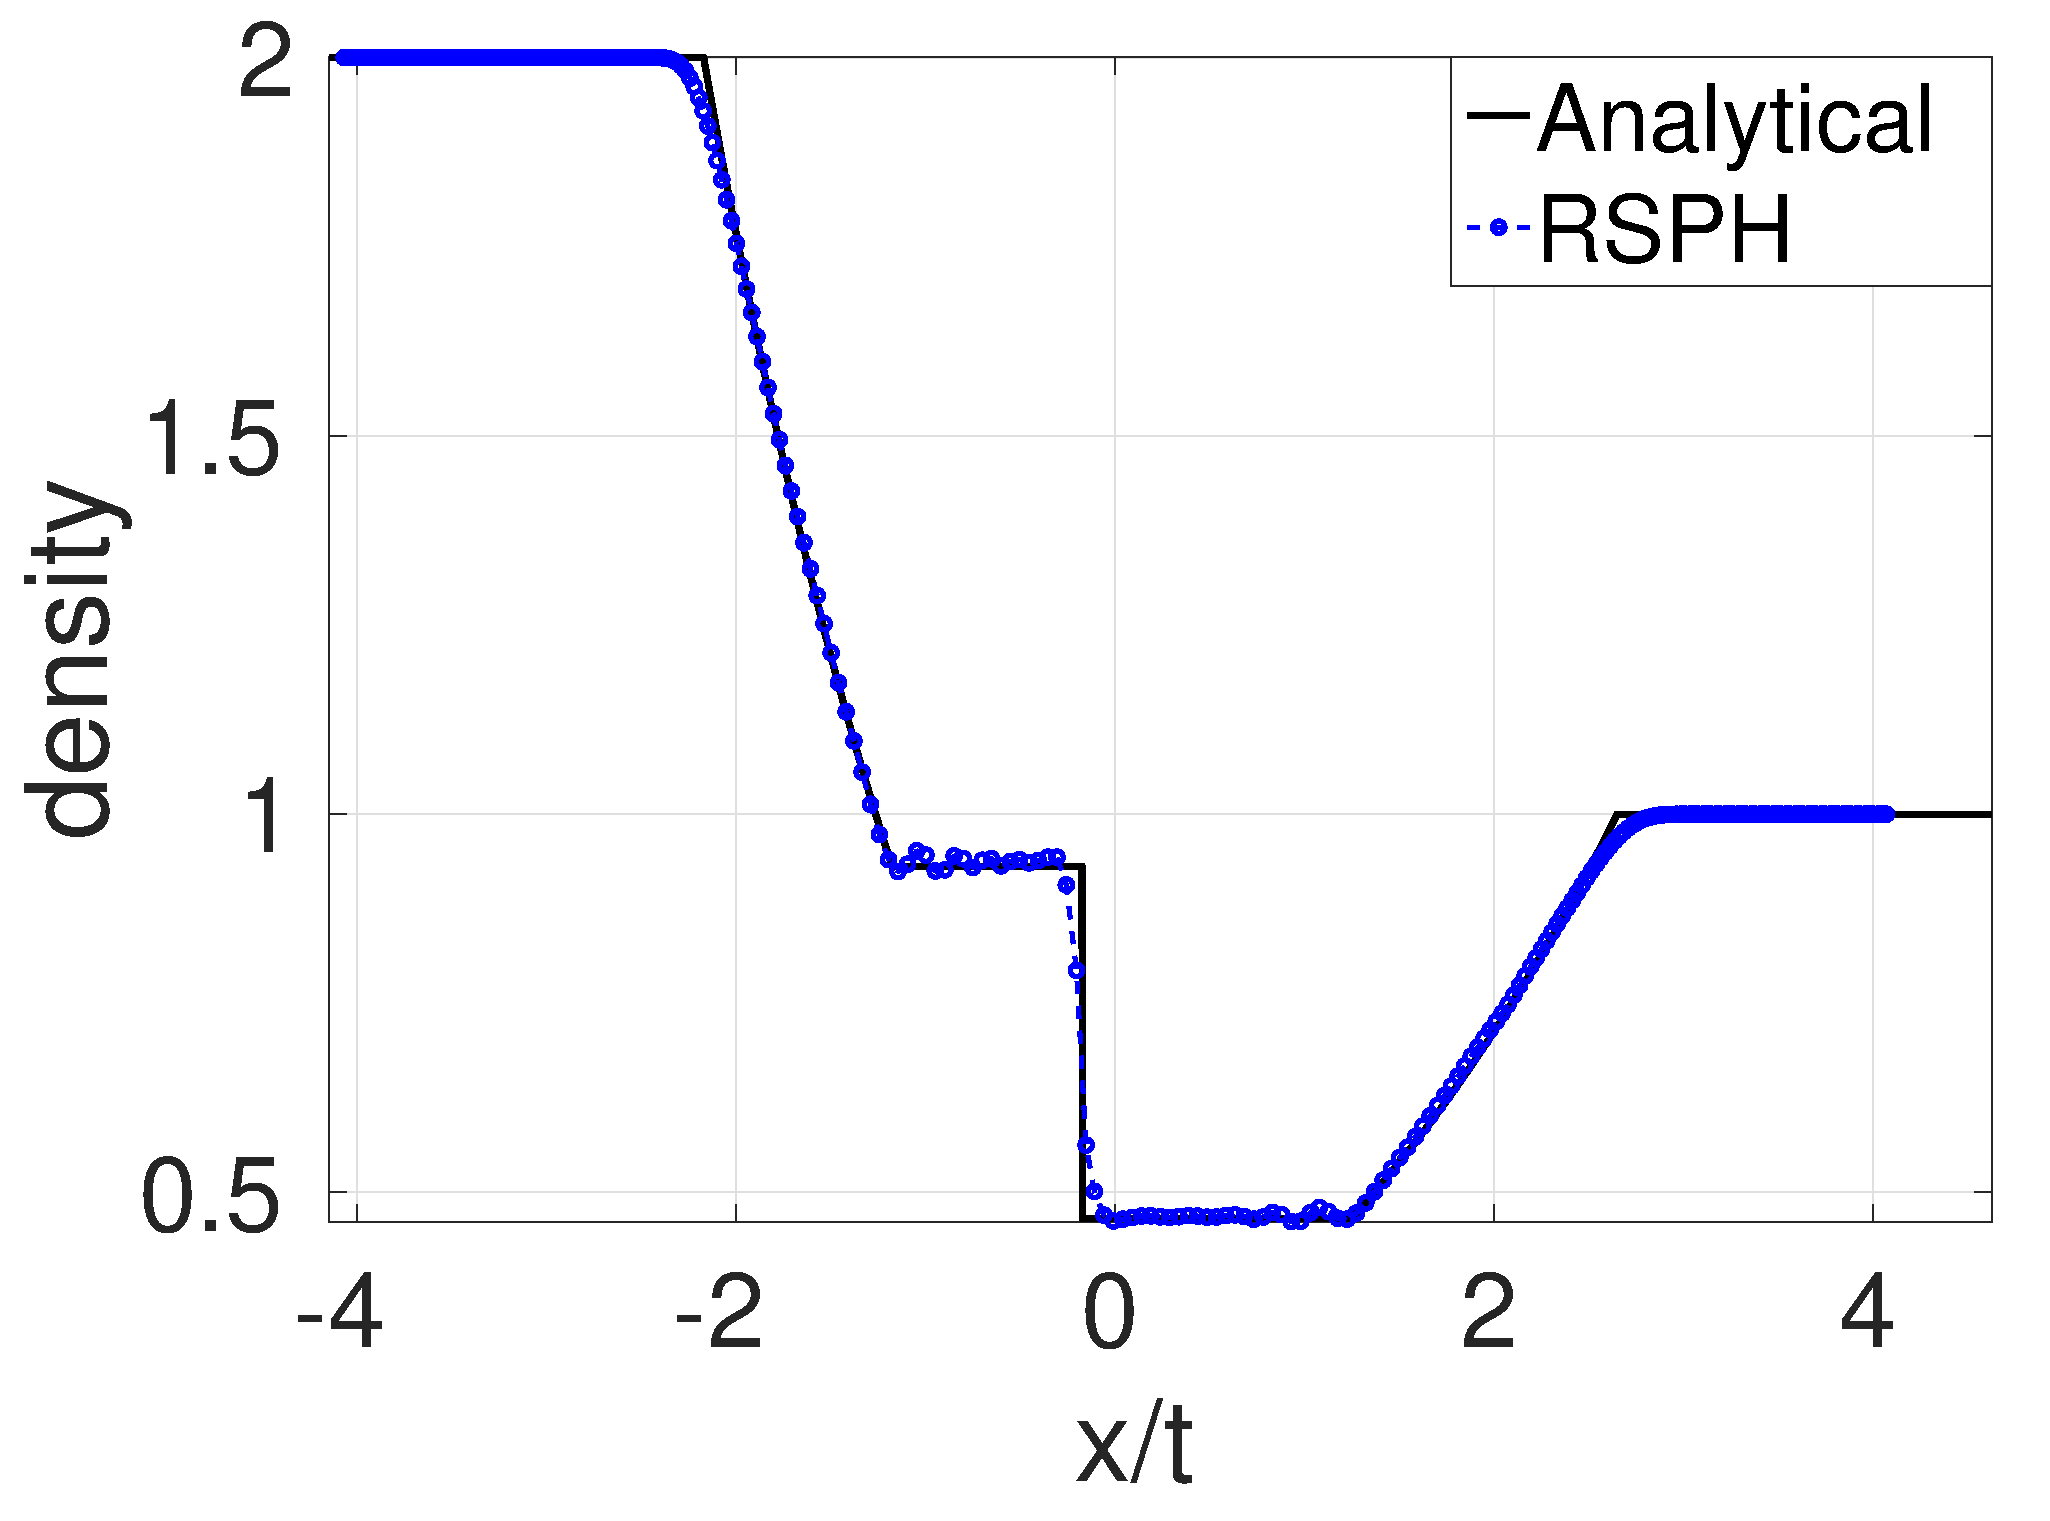
\includegraphics[width=0.99 \textwidth]{./Figures/double_exp/Dexp-RCM-rho}
    \end{minipage}%
    \begin{minipage}{.245 \textwidth}
        \centering
        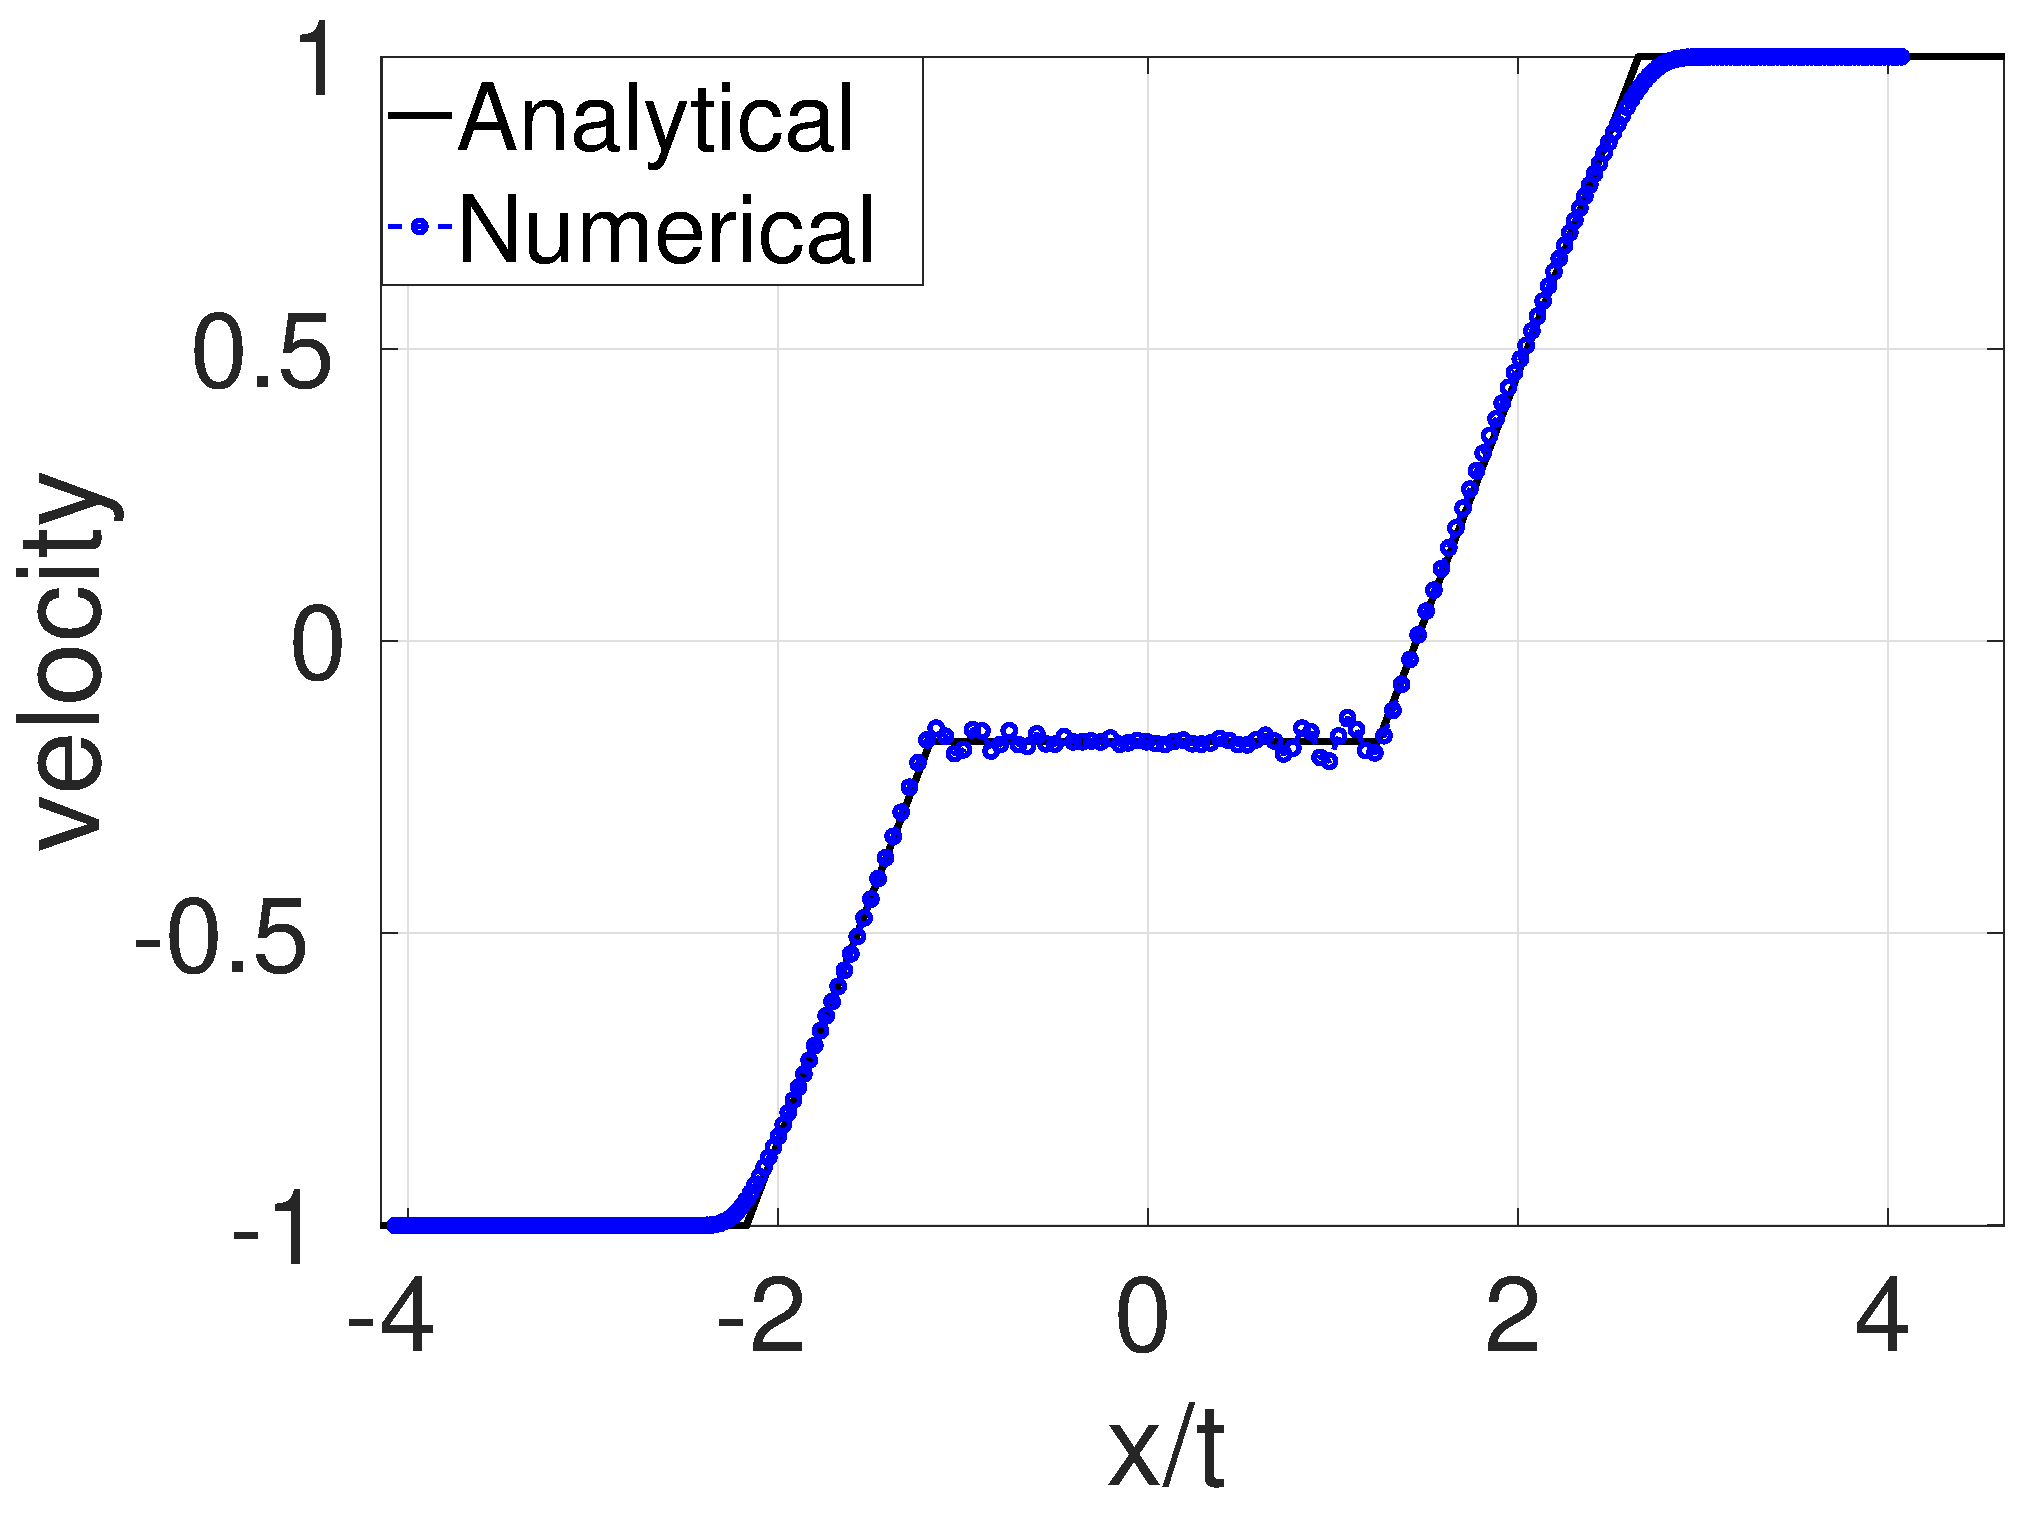
\includegraphics[width=0.99 \textwidth]{./Figures/double_exp/Dexp-RCM-v}
    \end{minipage}%
    \begin{minipage}{.245\textwidth}
        \centering
        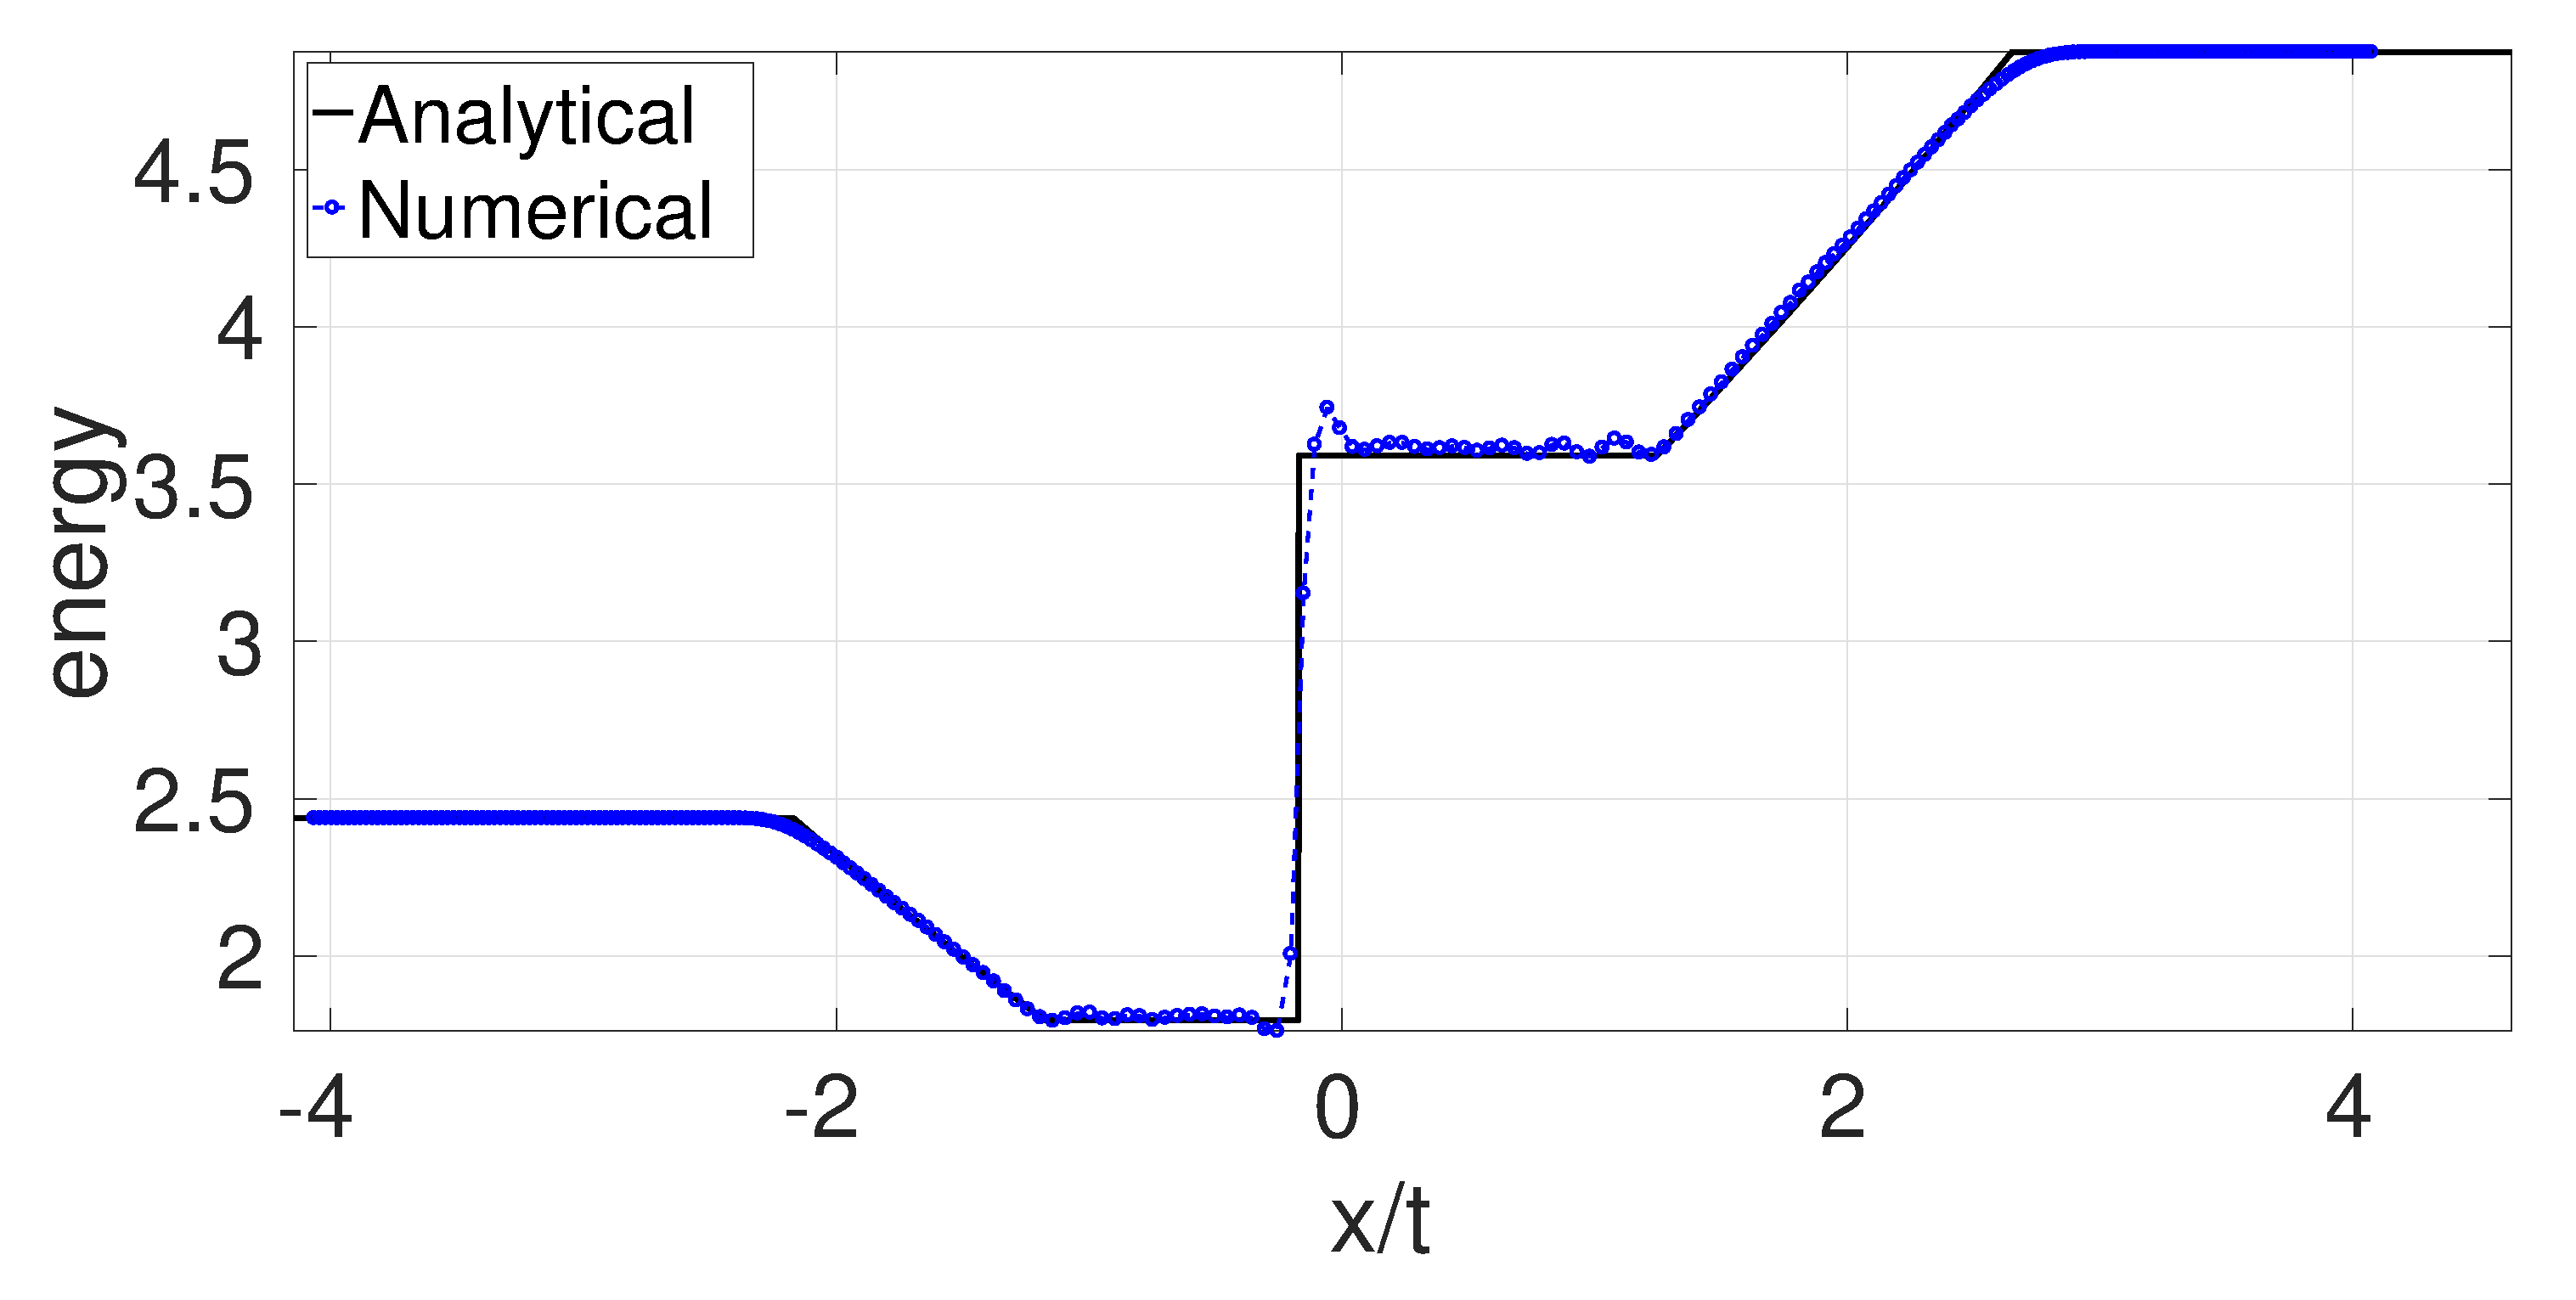
\includegraphics[width=0.99 \textwidth]{./Figures/double_exp/Dexp-RCM-e}
    \end{minipage}%
    \begin{minipage}{.245 \textwidth}
        \centering
        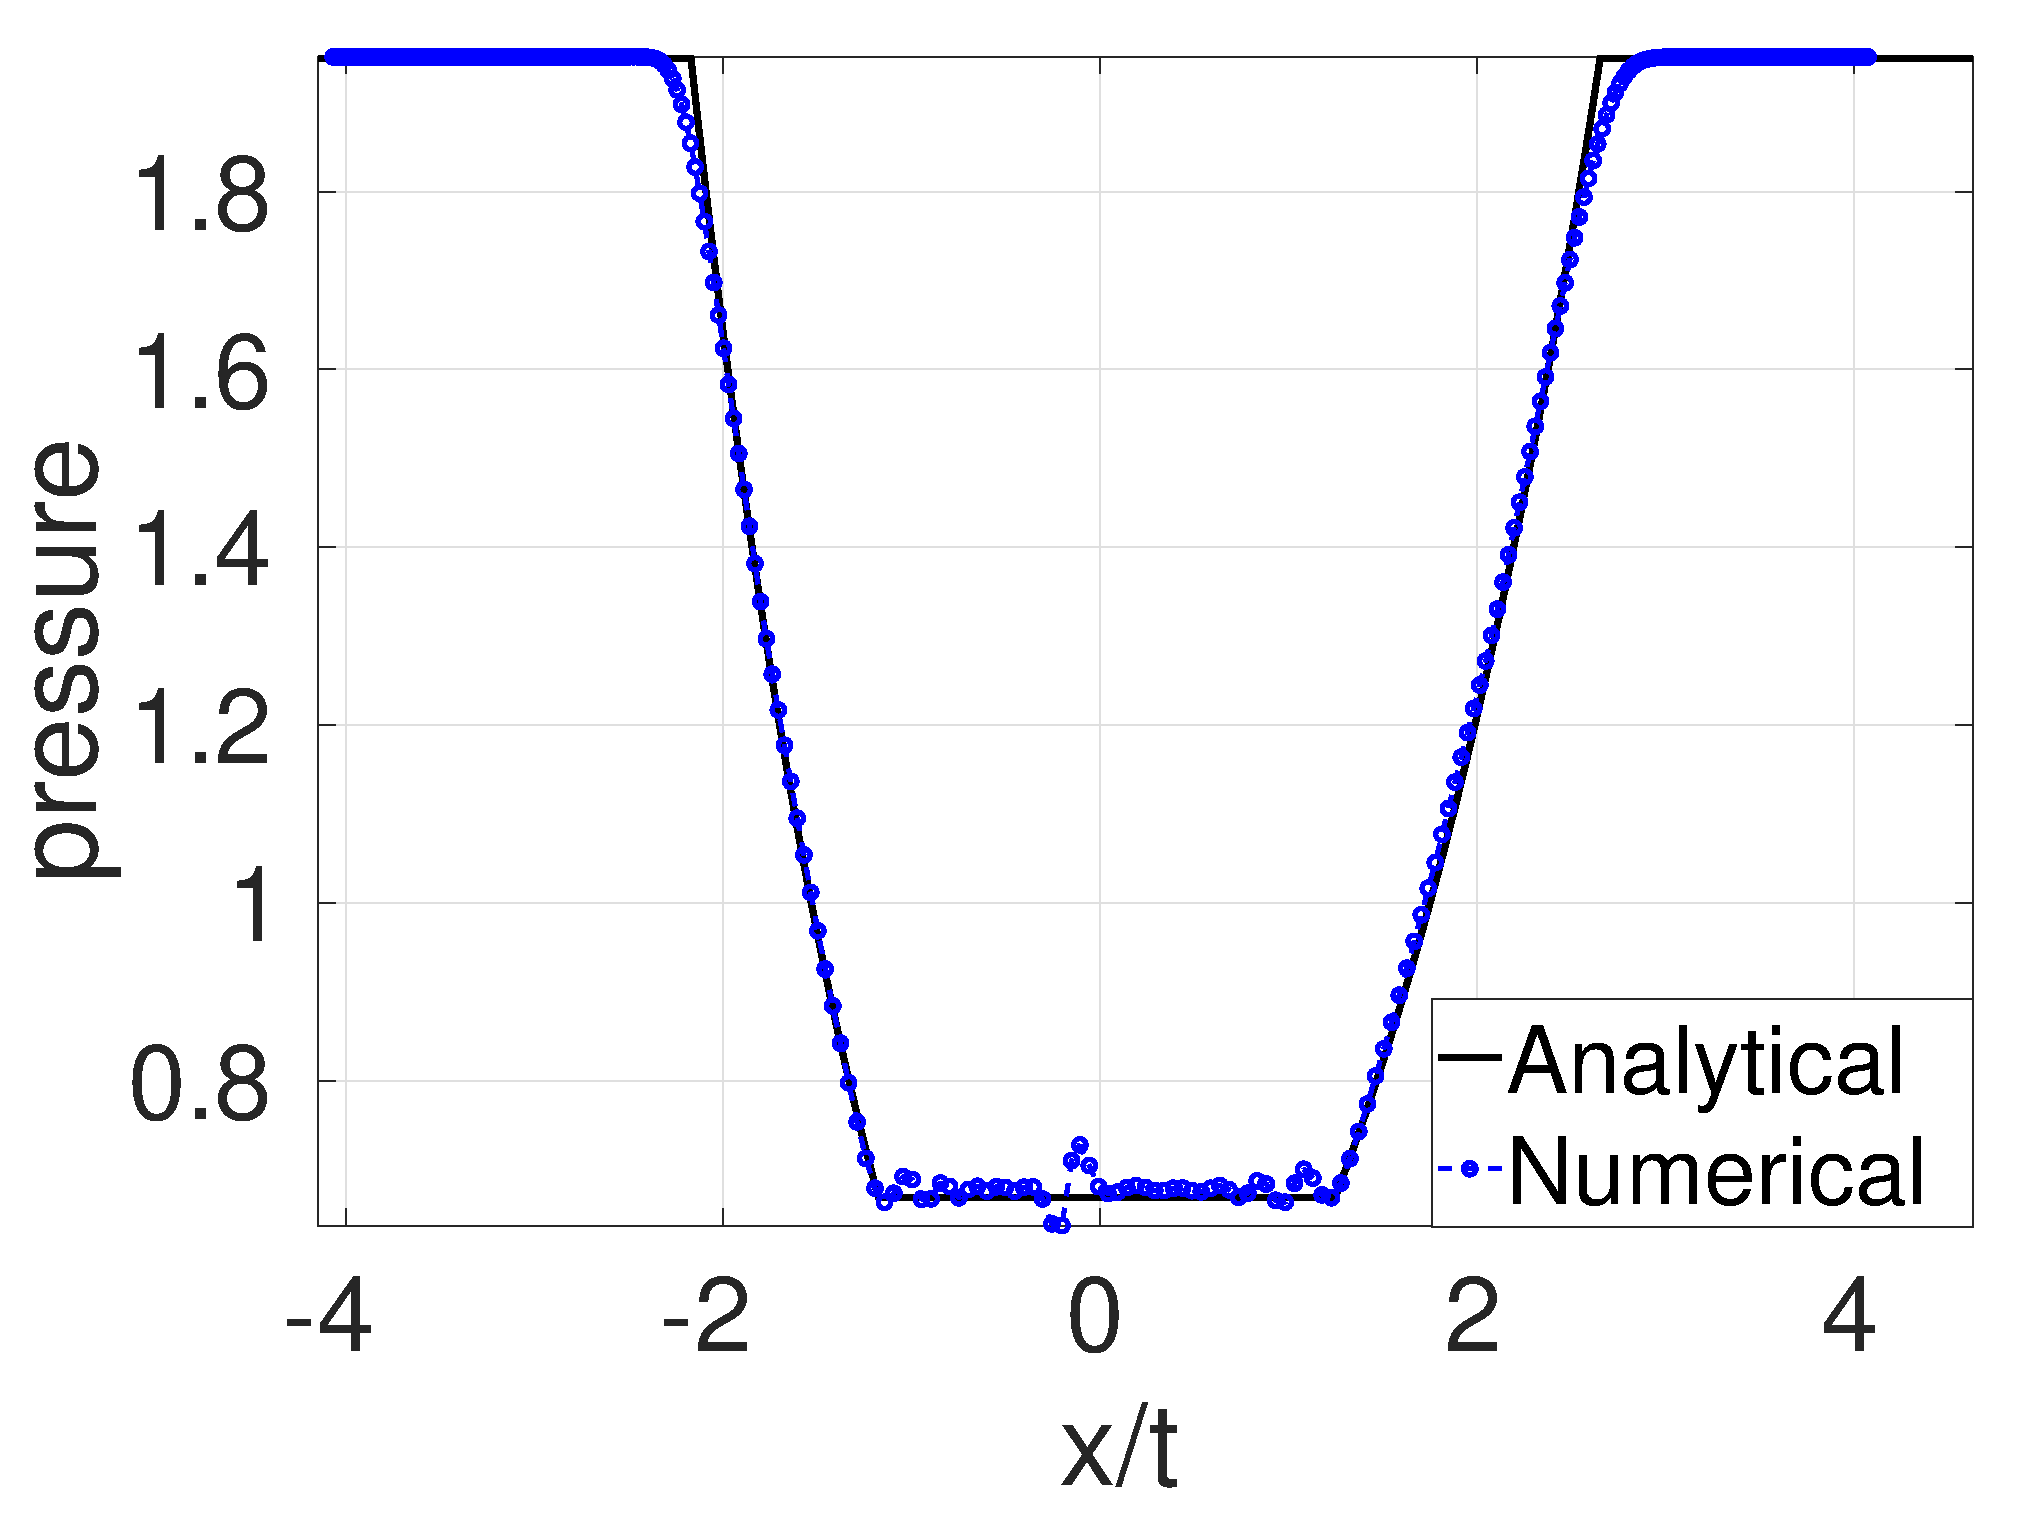
\includegraphics[width=0.99 \textwidth]{./Figures/double_exp/Dexp-RCM-p}
    \end{minipage}% 
    \caption{Results for test 3.}
    \label{fig:RCM-double-expansion}
\end{figure}
\begin{figure}[H]
    %\centering
    \begin{minipage}{.245\textwidth}
        \centering
        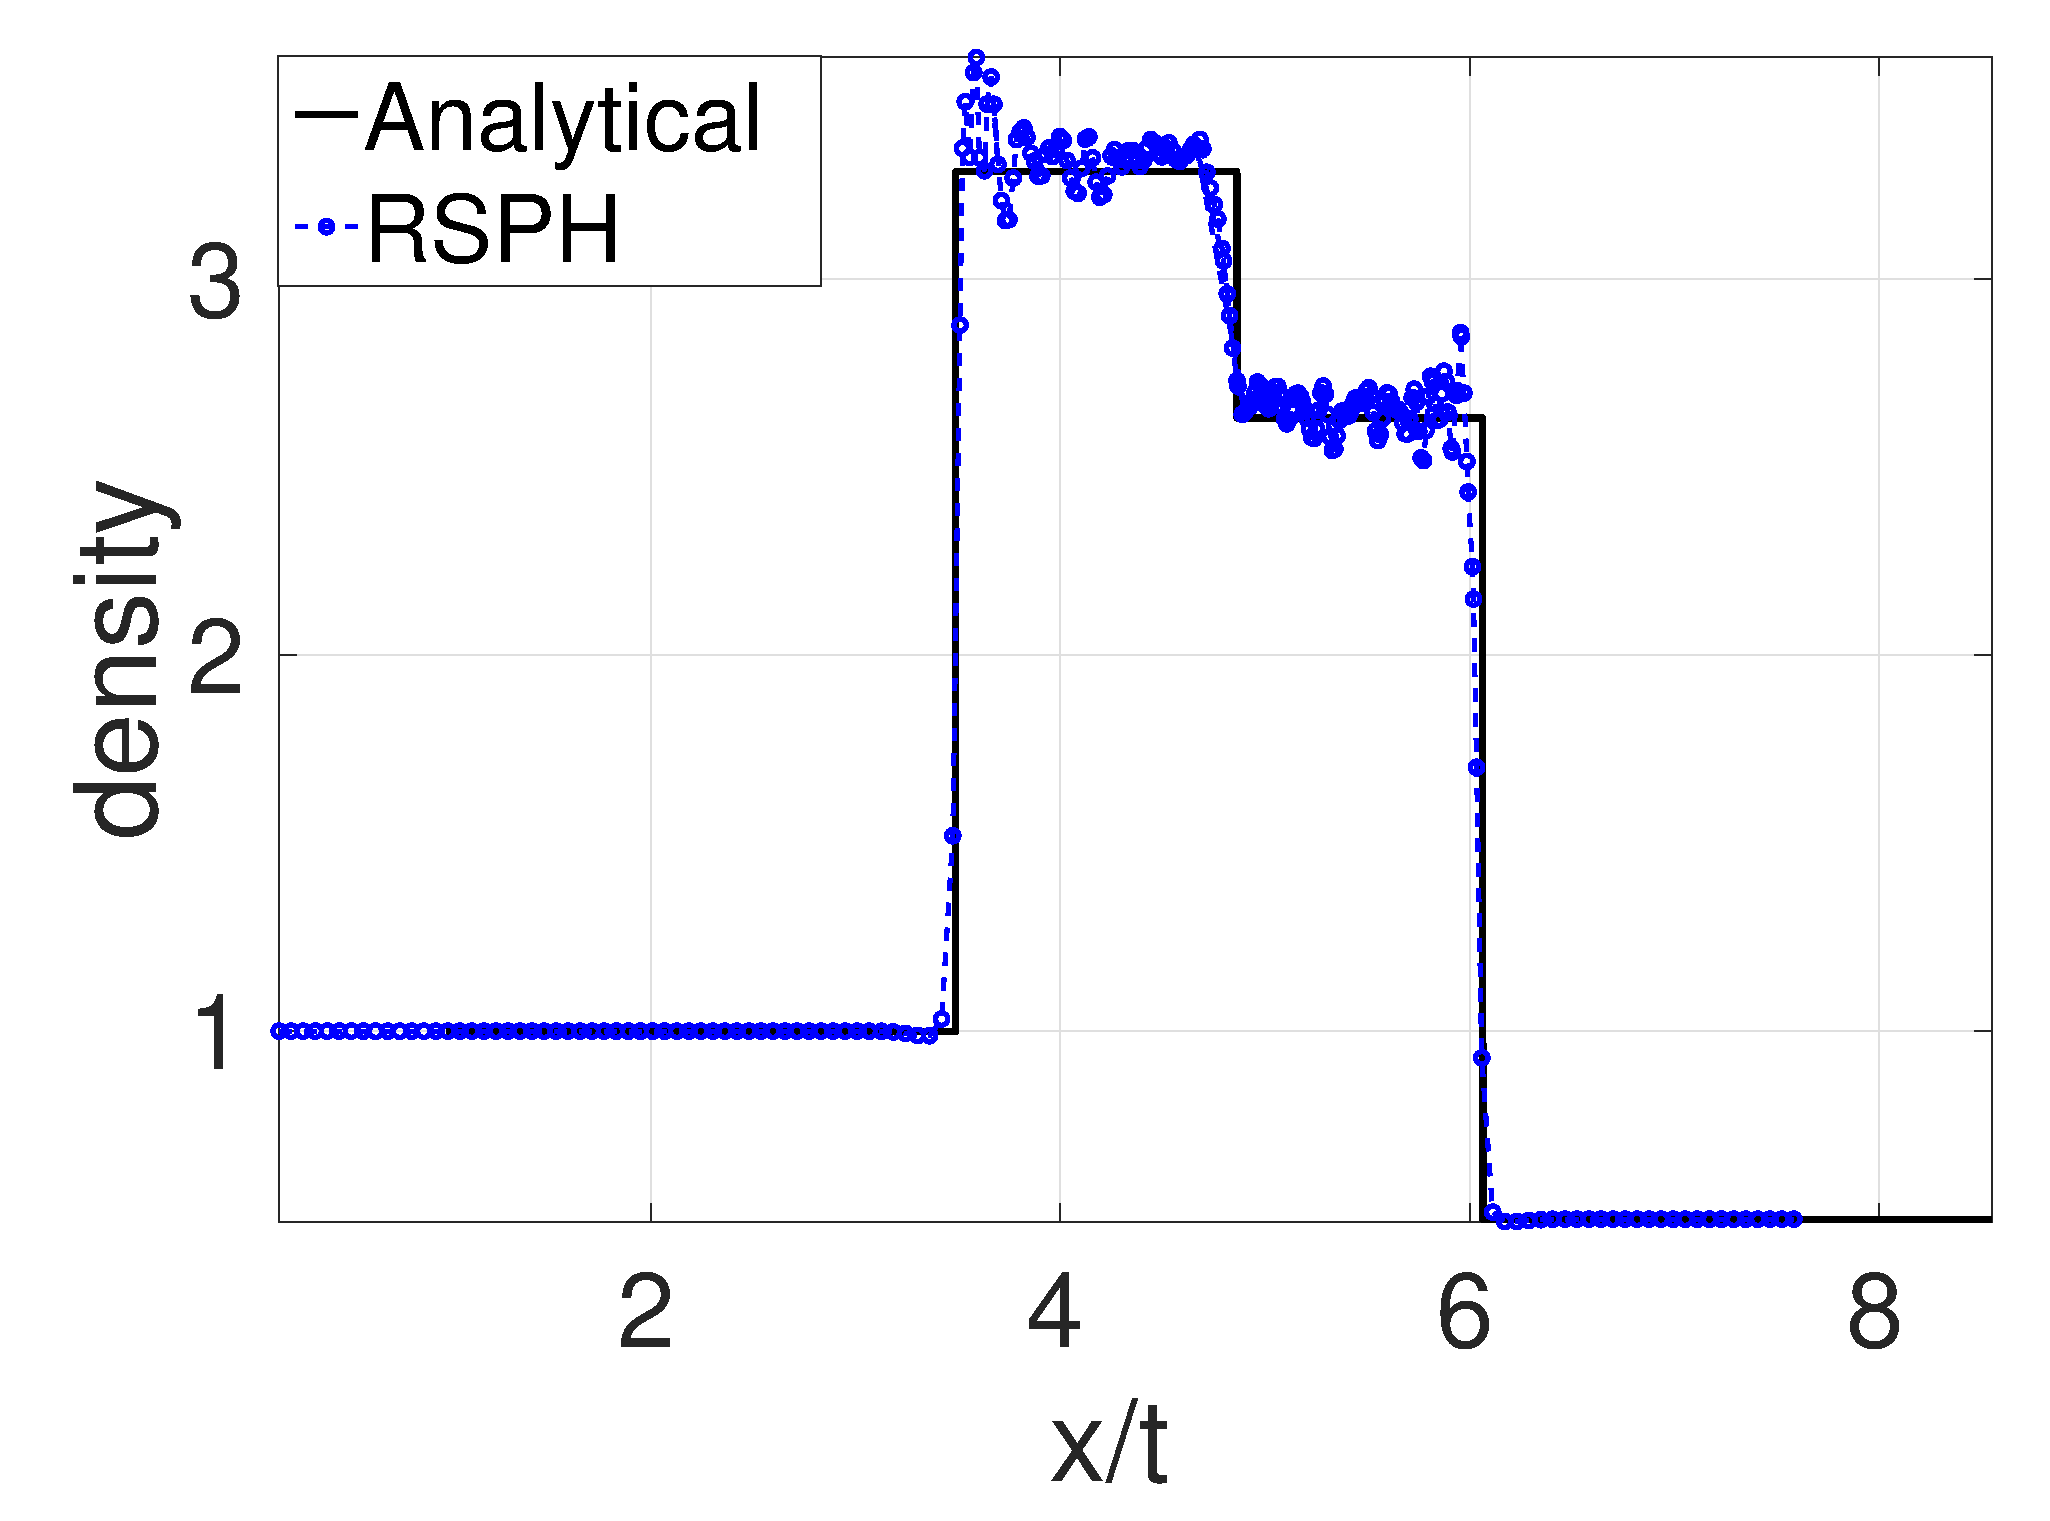
\includegraphics[width=0.99 \textwidth]{./Figures/double_shock/Dshock-RCM-rho-Rp6}
    \end{minipage}%
    \begin{minipage}{.245 \textwidth}
        \centering
        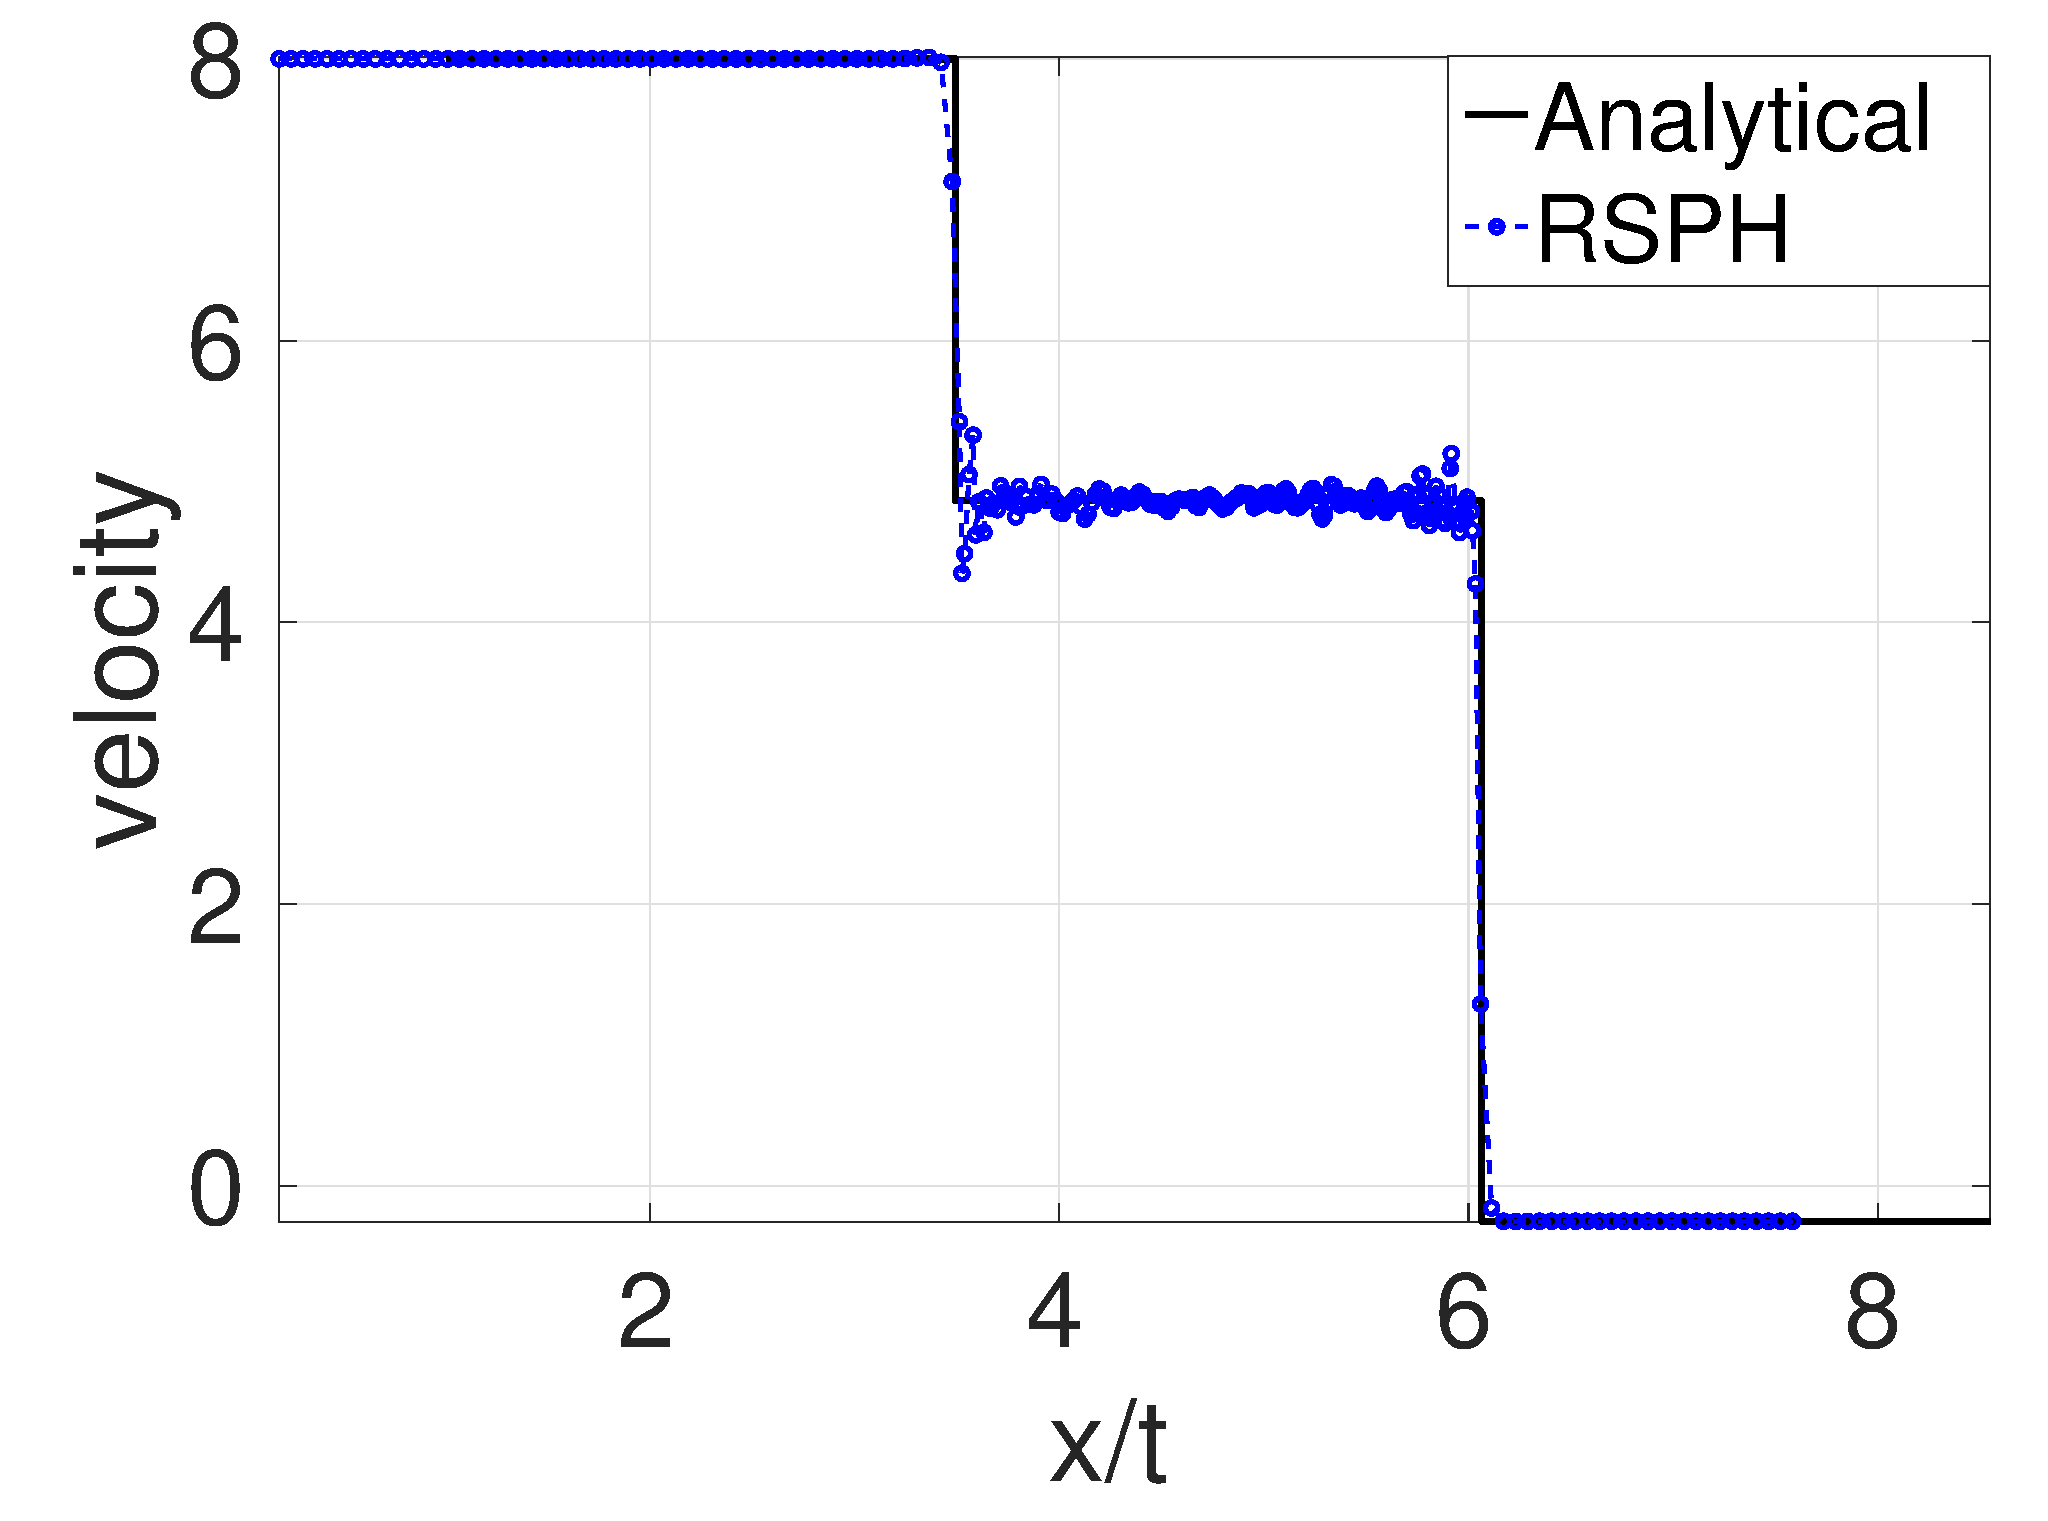
\includegraphics[width=0.99 \textwidth]{./Figures/double_shock/Dshock-RCM-v-Rp6}
    \end{minipage}%
    \begin{minipage}{.245\textwidth}
        \centering
        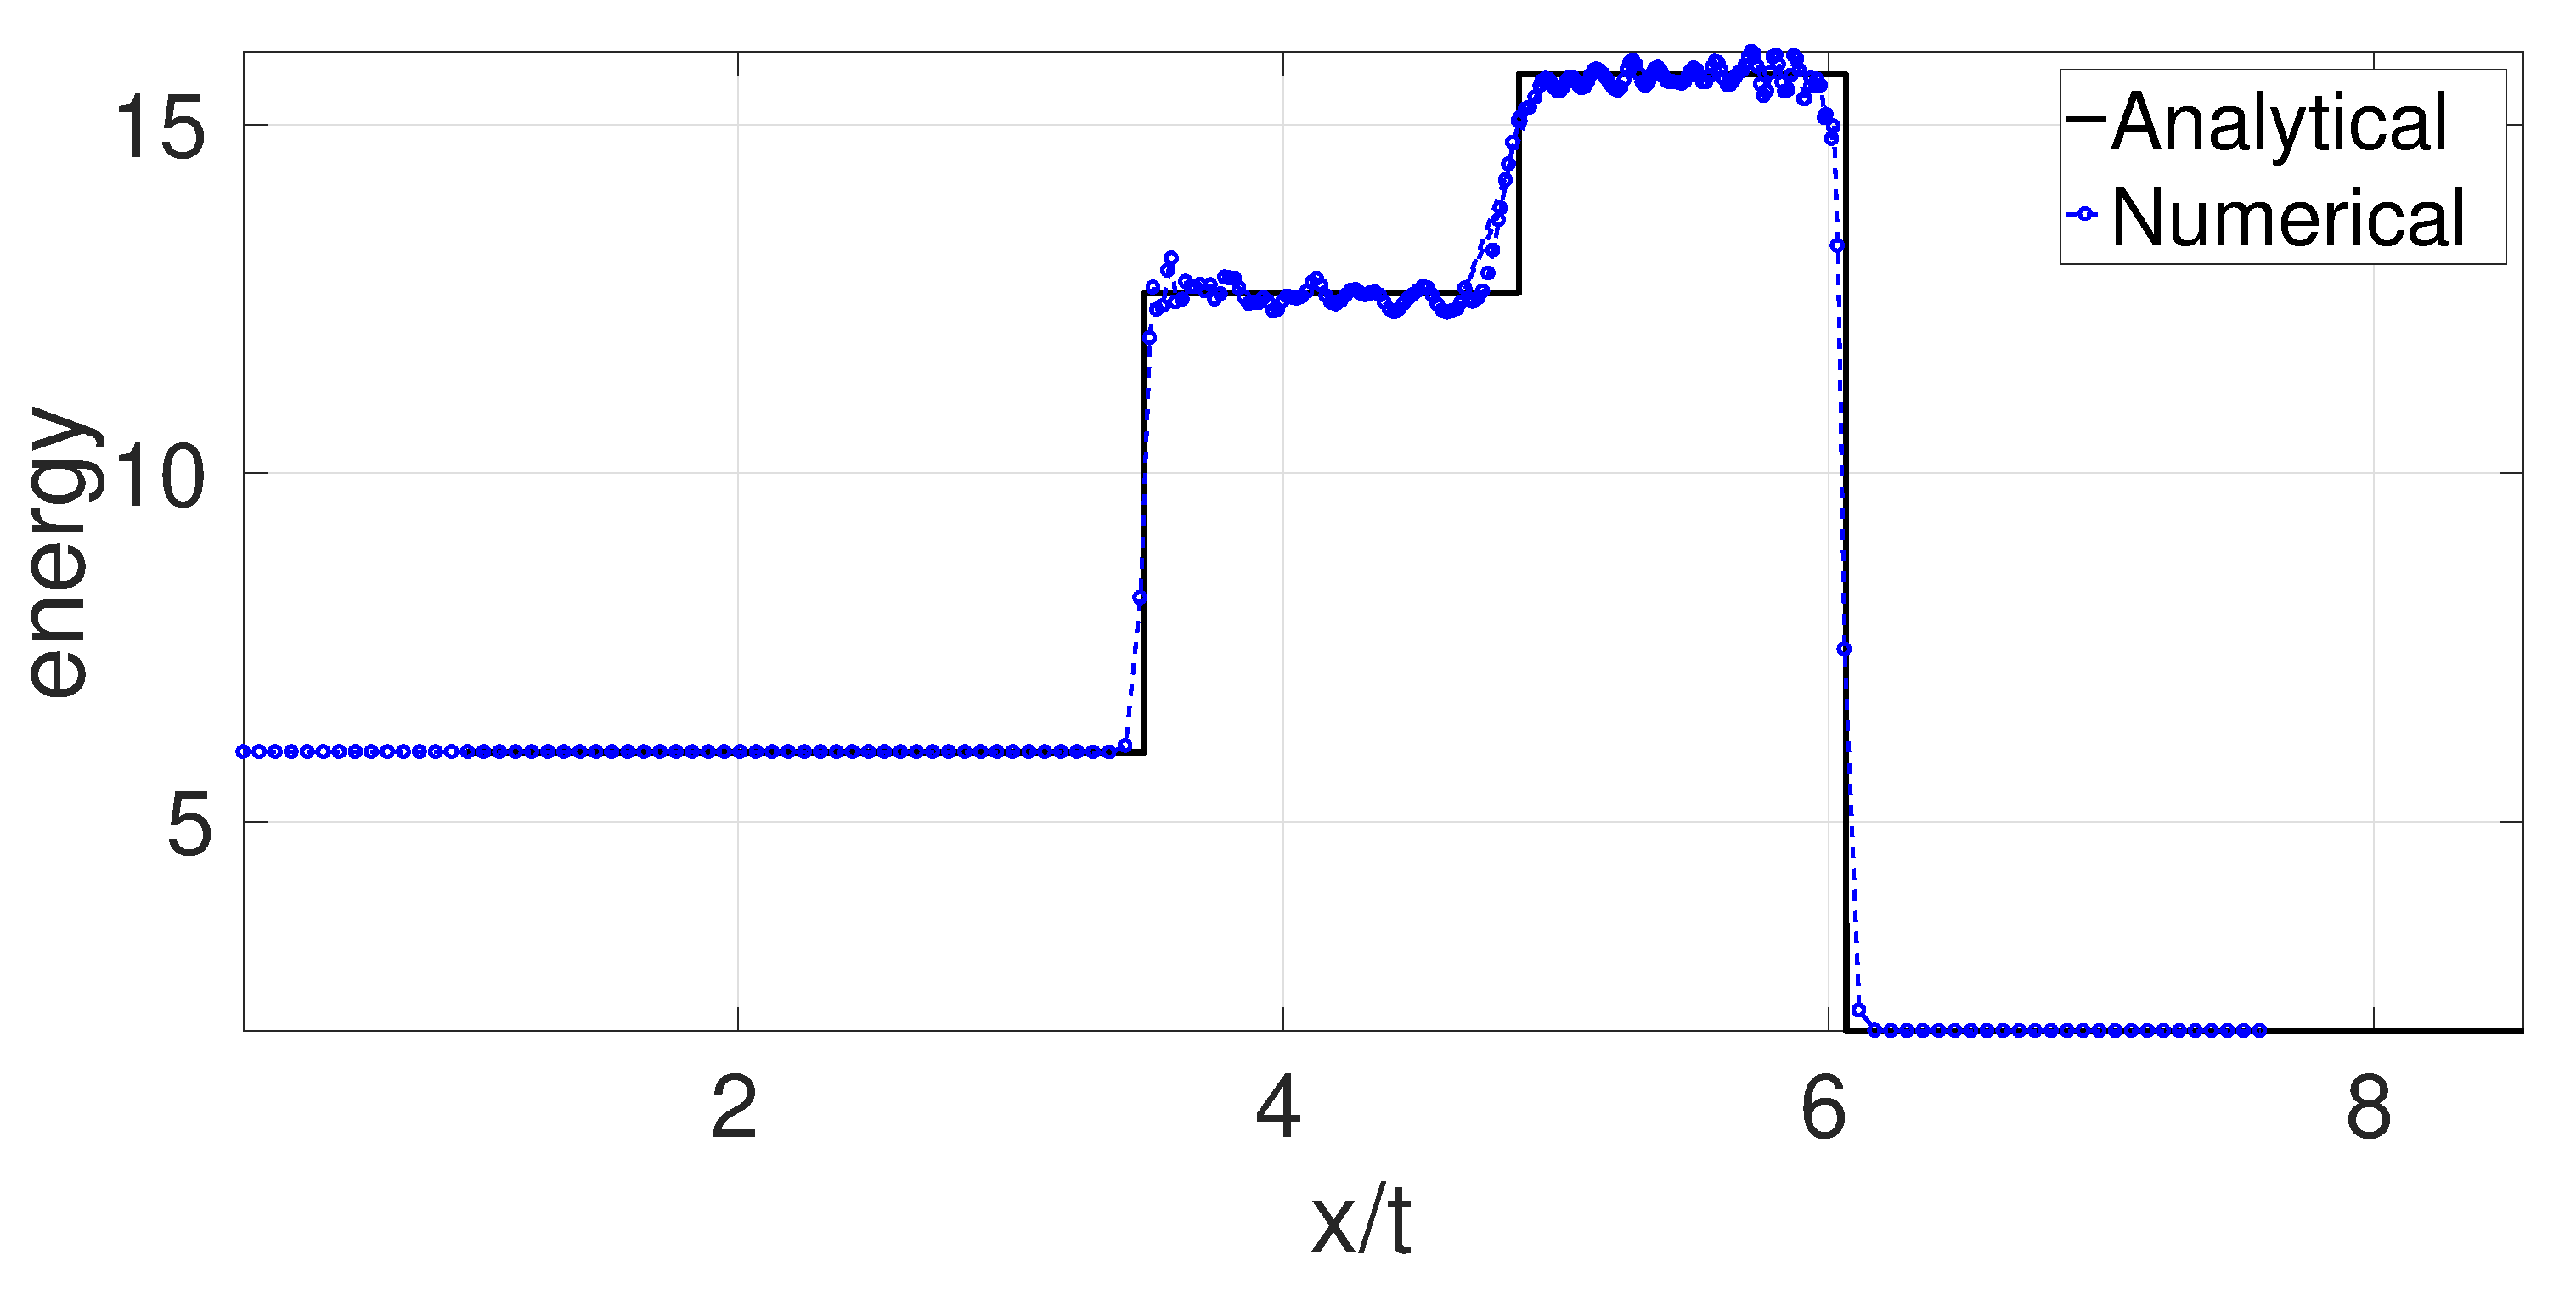
\includegraphics[width=0.99 \textwidth]{./Figures/double_shock/Dshock-RCM-e-Rp6}
    \end{minipage}%
    \begin{minipage}{.245 \textwidth}
        \centering
        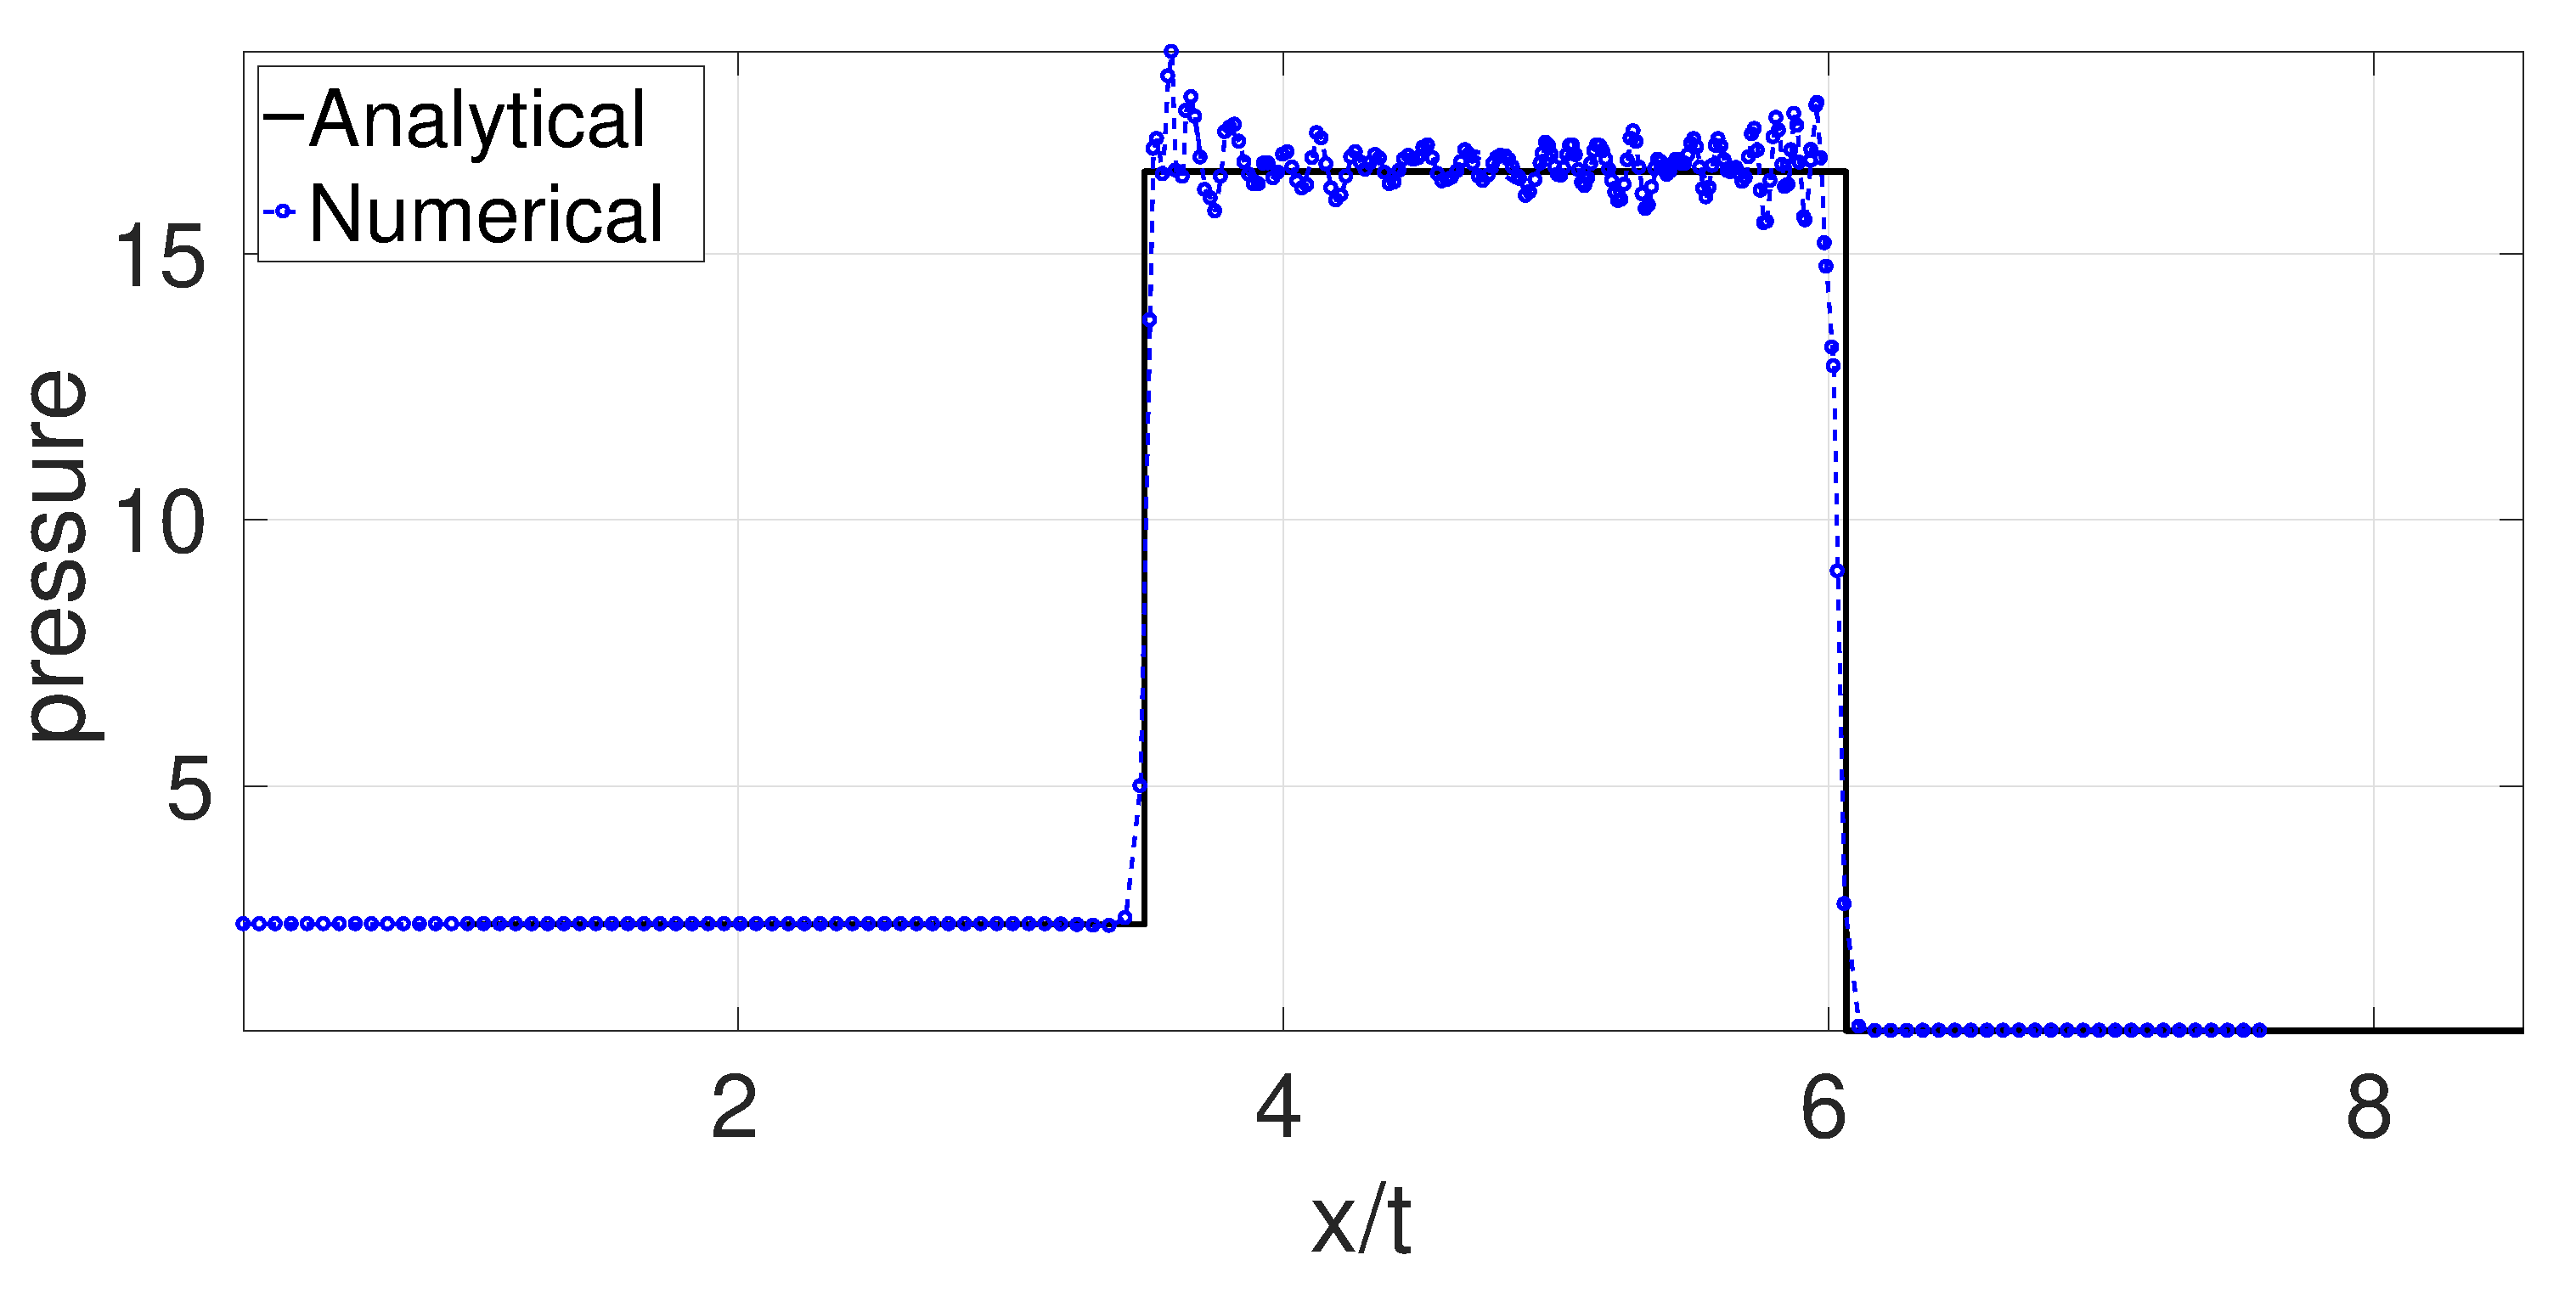
\includegraphics[width=0.99 \textwidth]{./Figures/double_shock/Dshock-RCM-p-Rp6}
    \end{minipage}% 
    \caption{Results for test 4. The fluctuations are more serious than other tests}
    \label{fig:RCM-double-shock}
\end{figure}
\begin{figure}[H]
    %\centering
    \begin{minipage}{.245\textwidth}
        \centering
        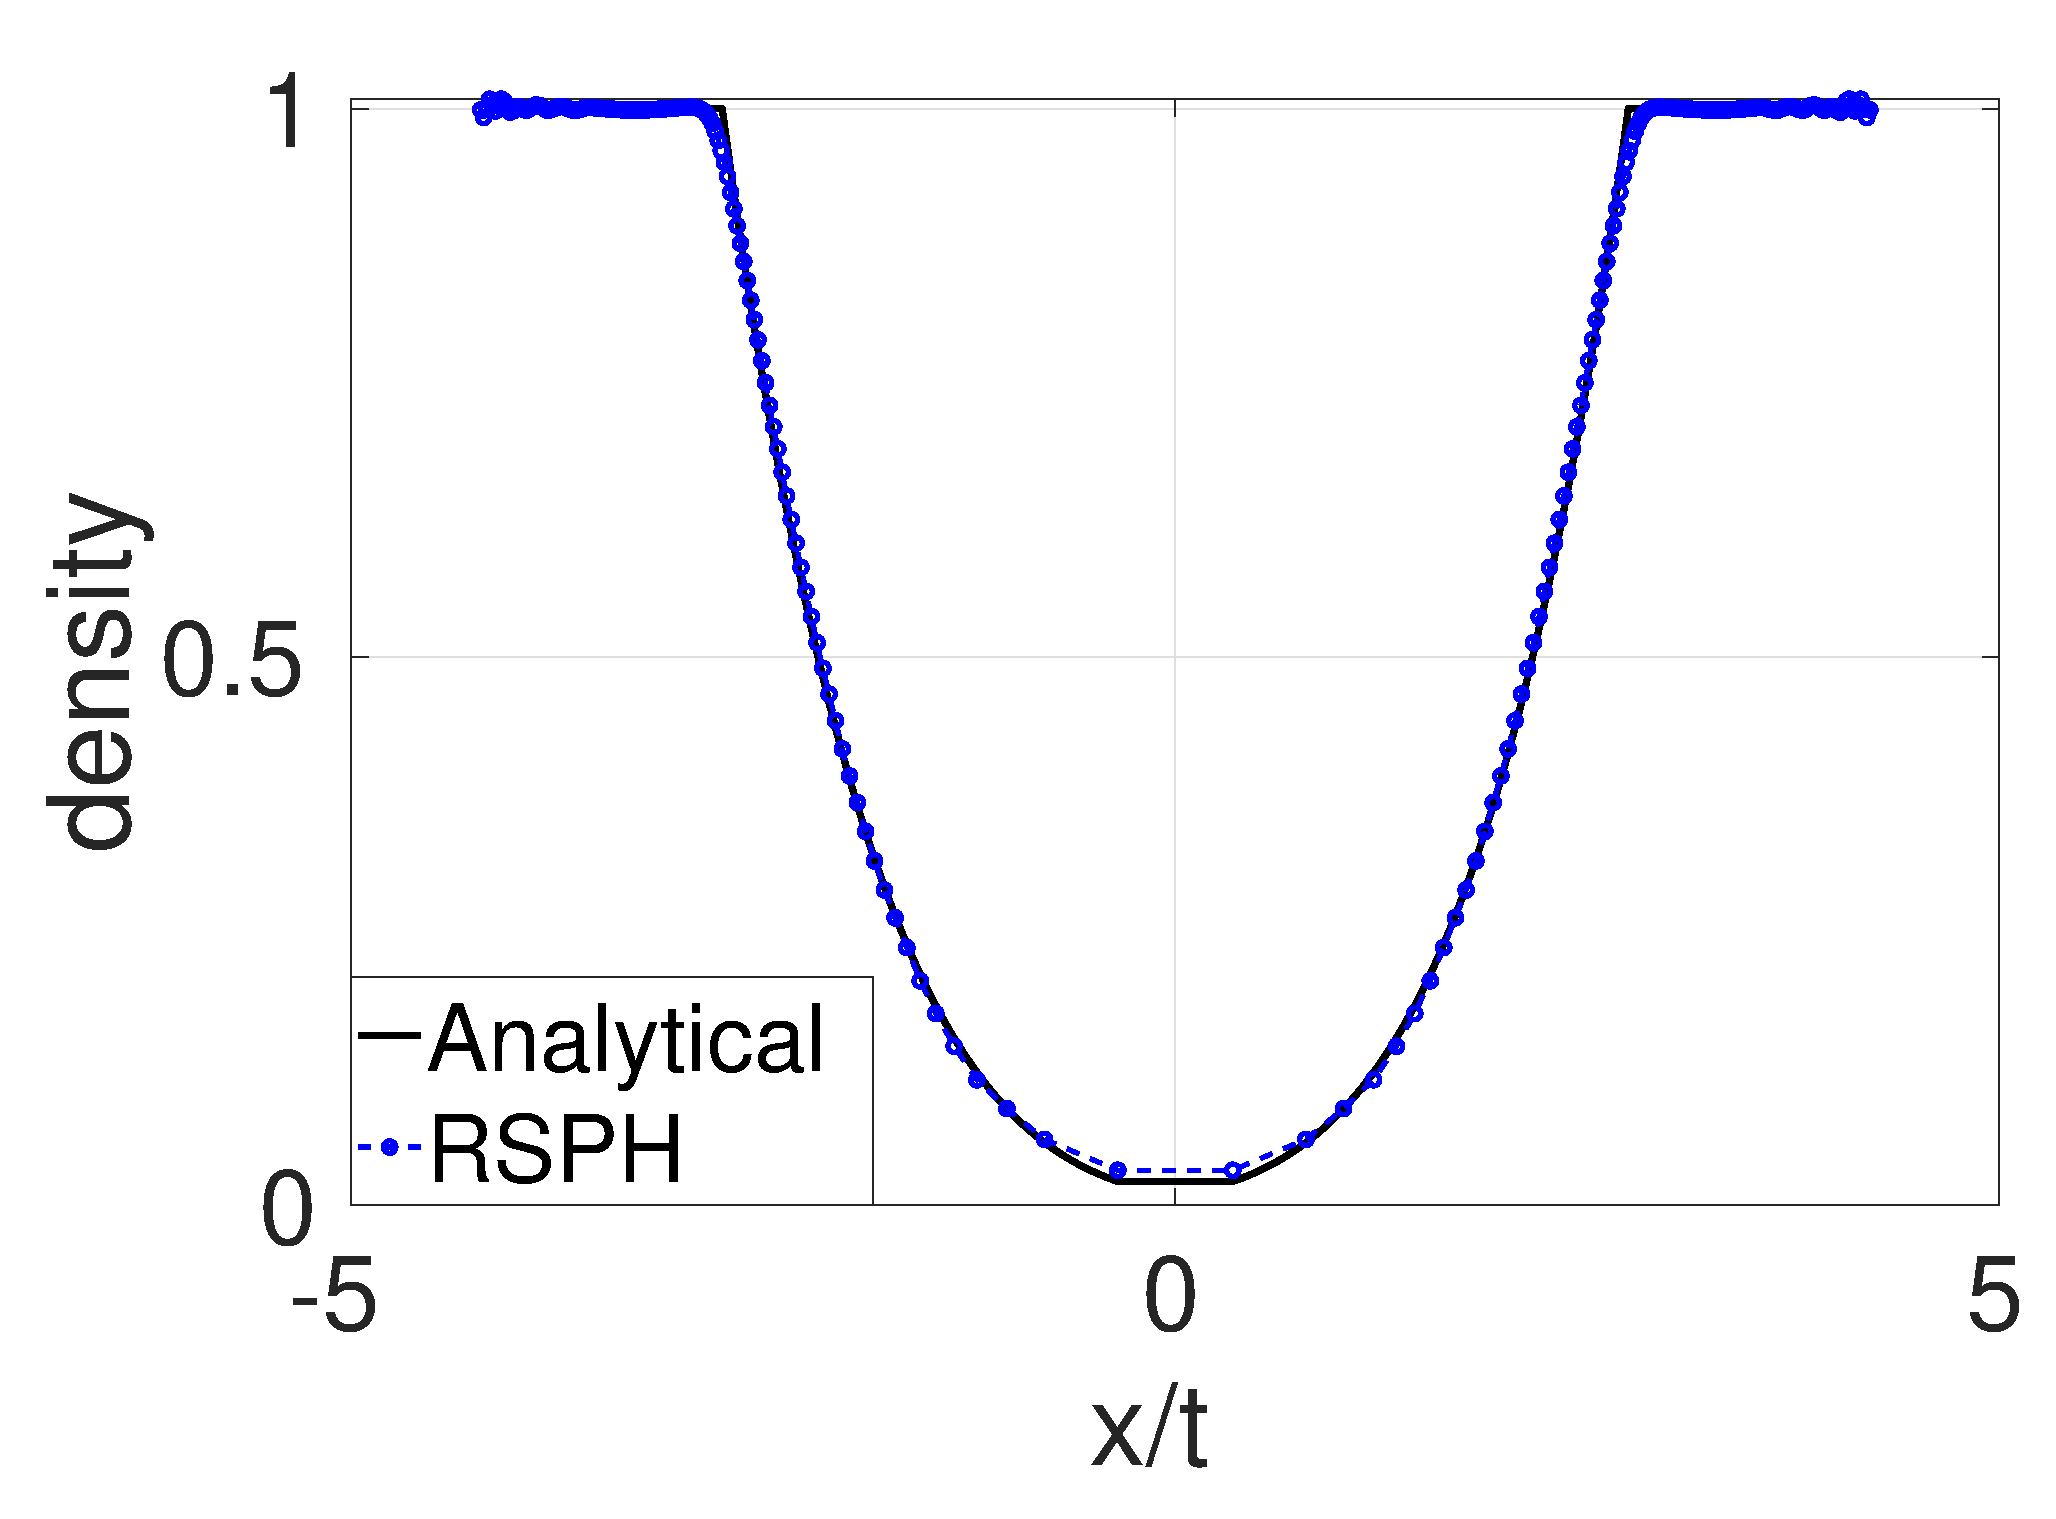
\includegraphics[width=0.99 \textwidth]{./Figures/Sjogreen/Sjogreen-RCM-rho-Adpt1}
    \end{minipage}%
    \begin{minipage}{.245 \textwidth}
        \centering
        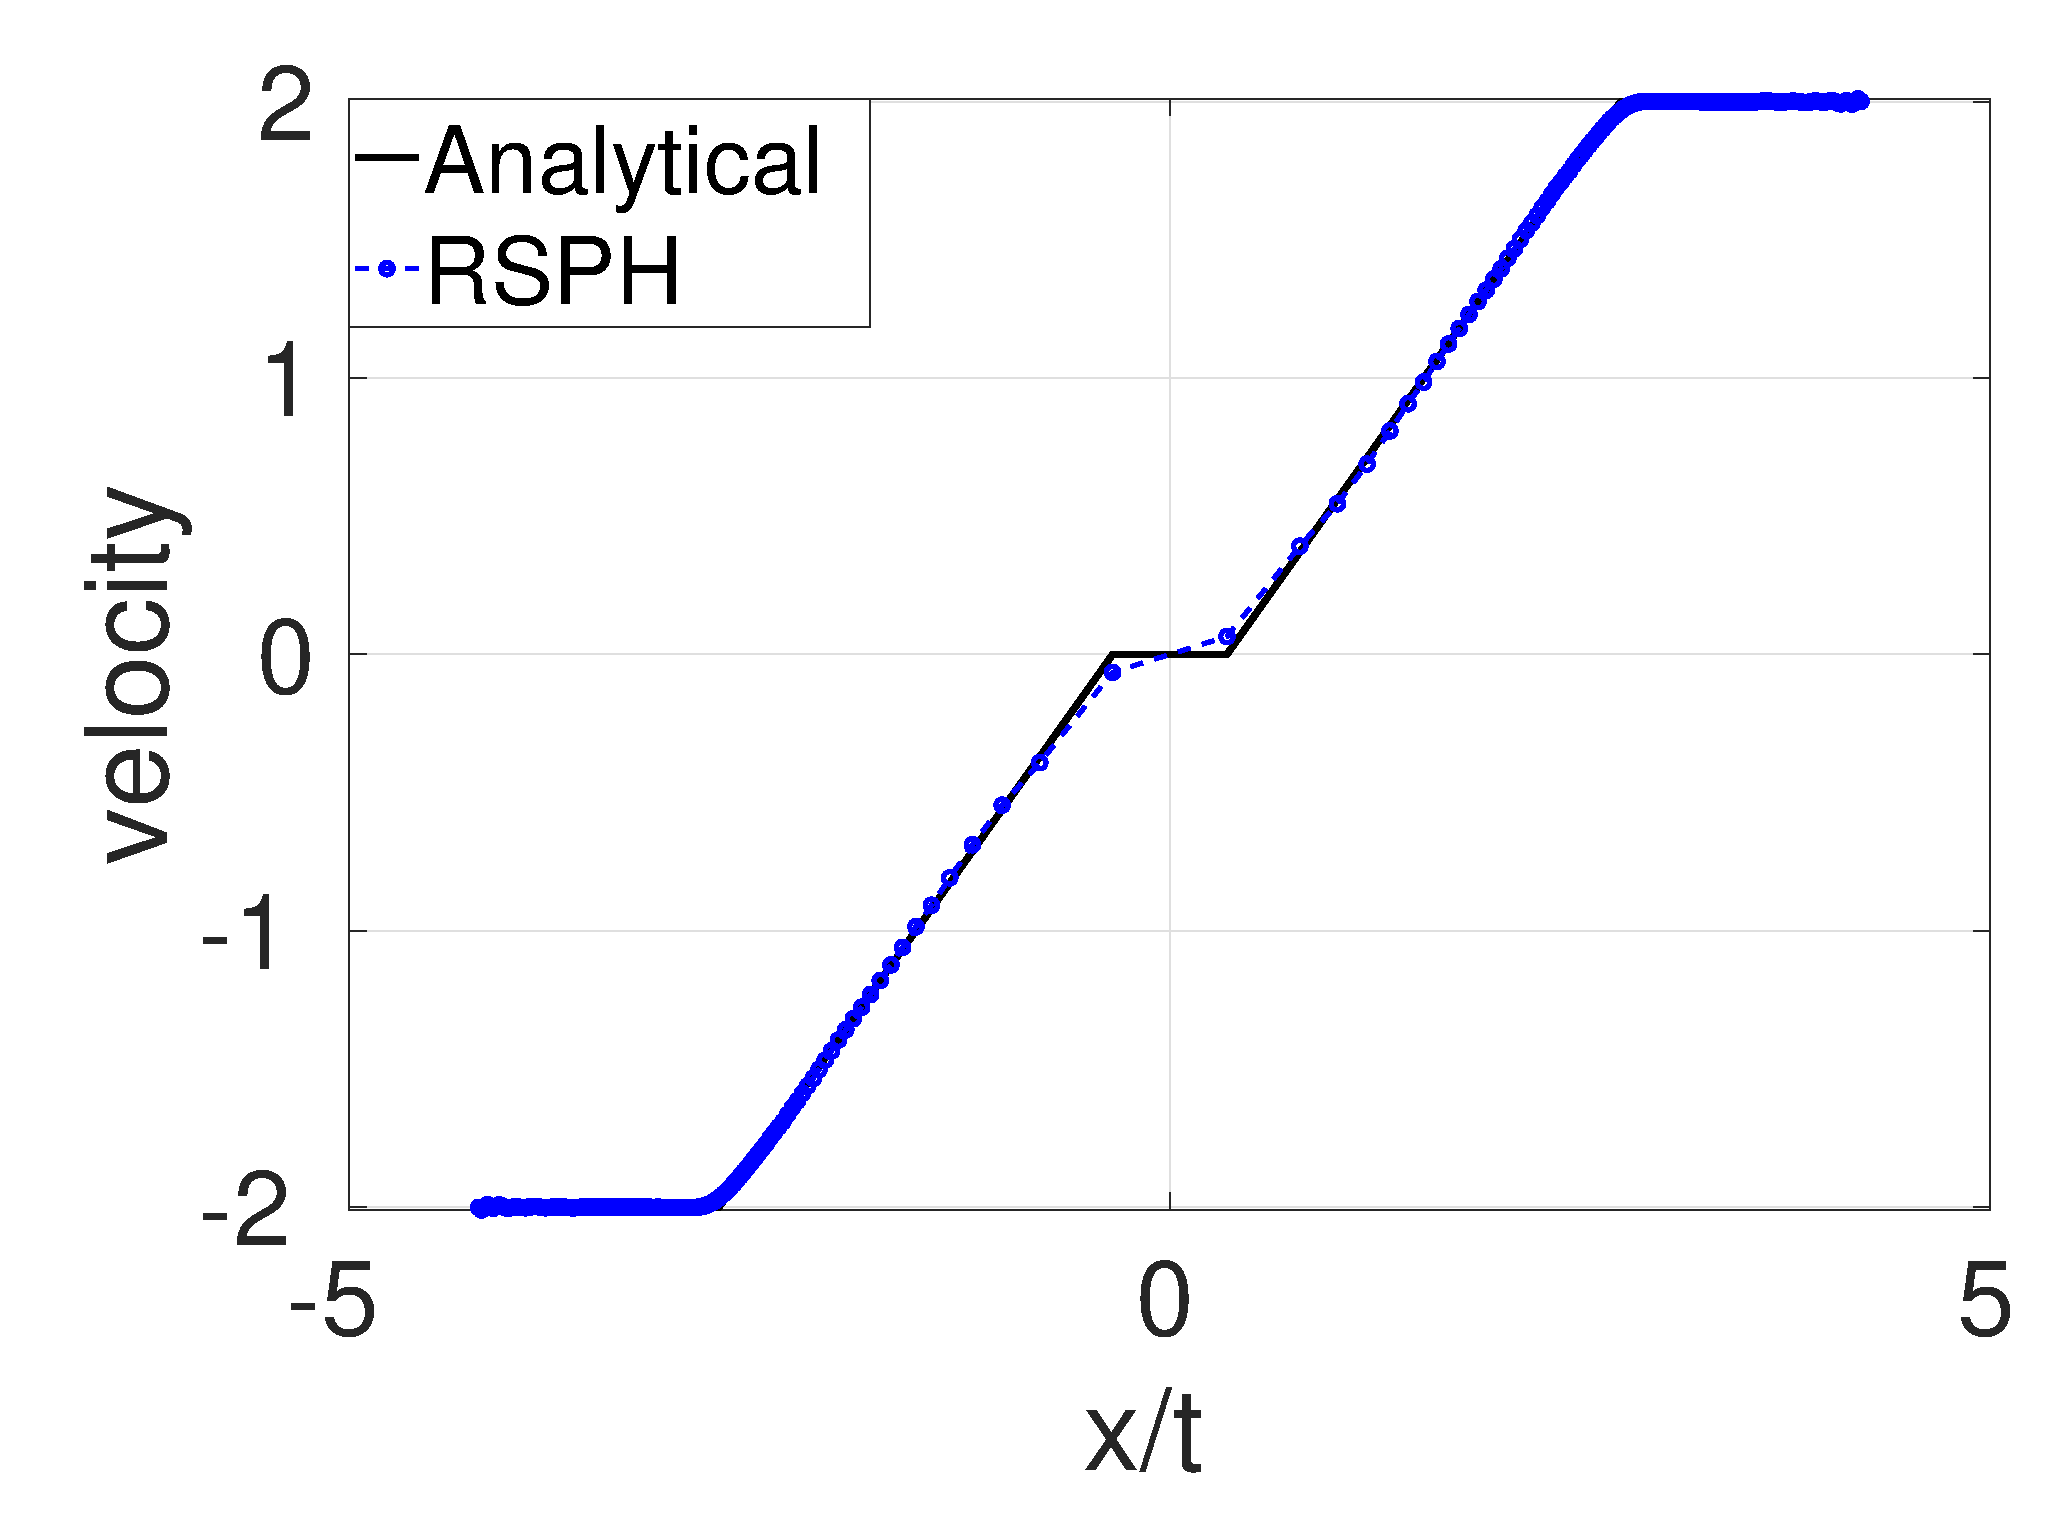
\includegraphics[width=0.99 \textwidth]{./Figures/Sjogreen/Sjogreen-RCM-v-Adpt1}
    \end{minipage}%
    \begin{minipage}{.245\textwidth}
        \centering
        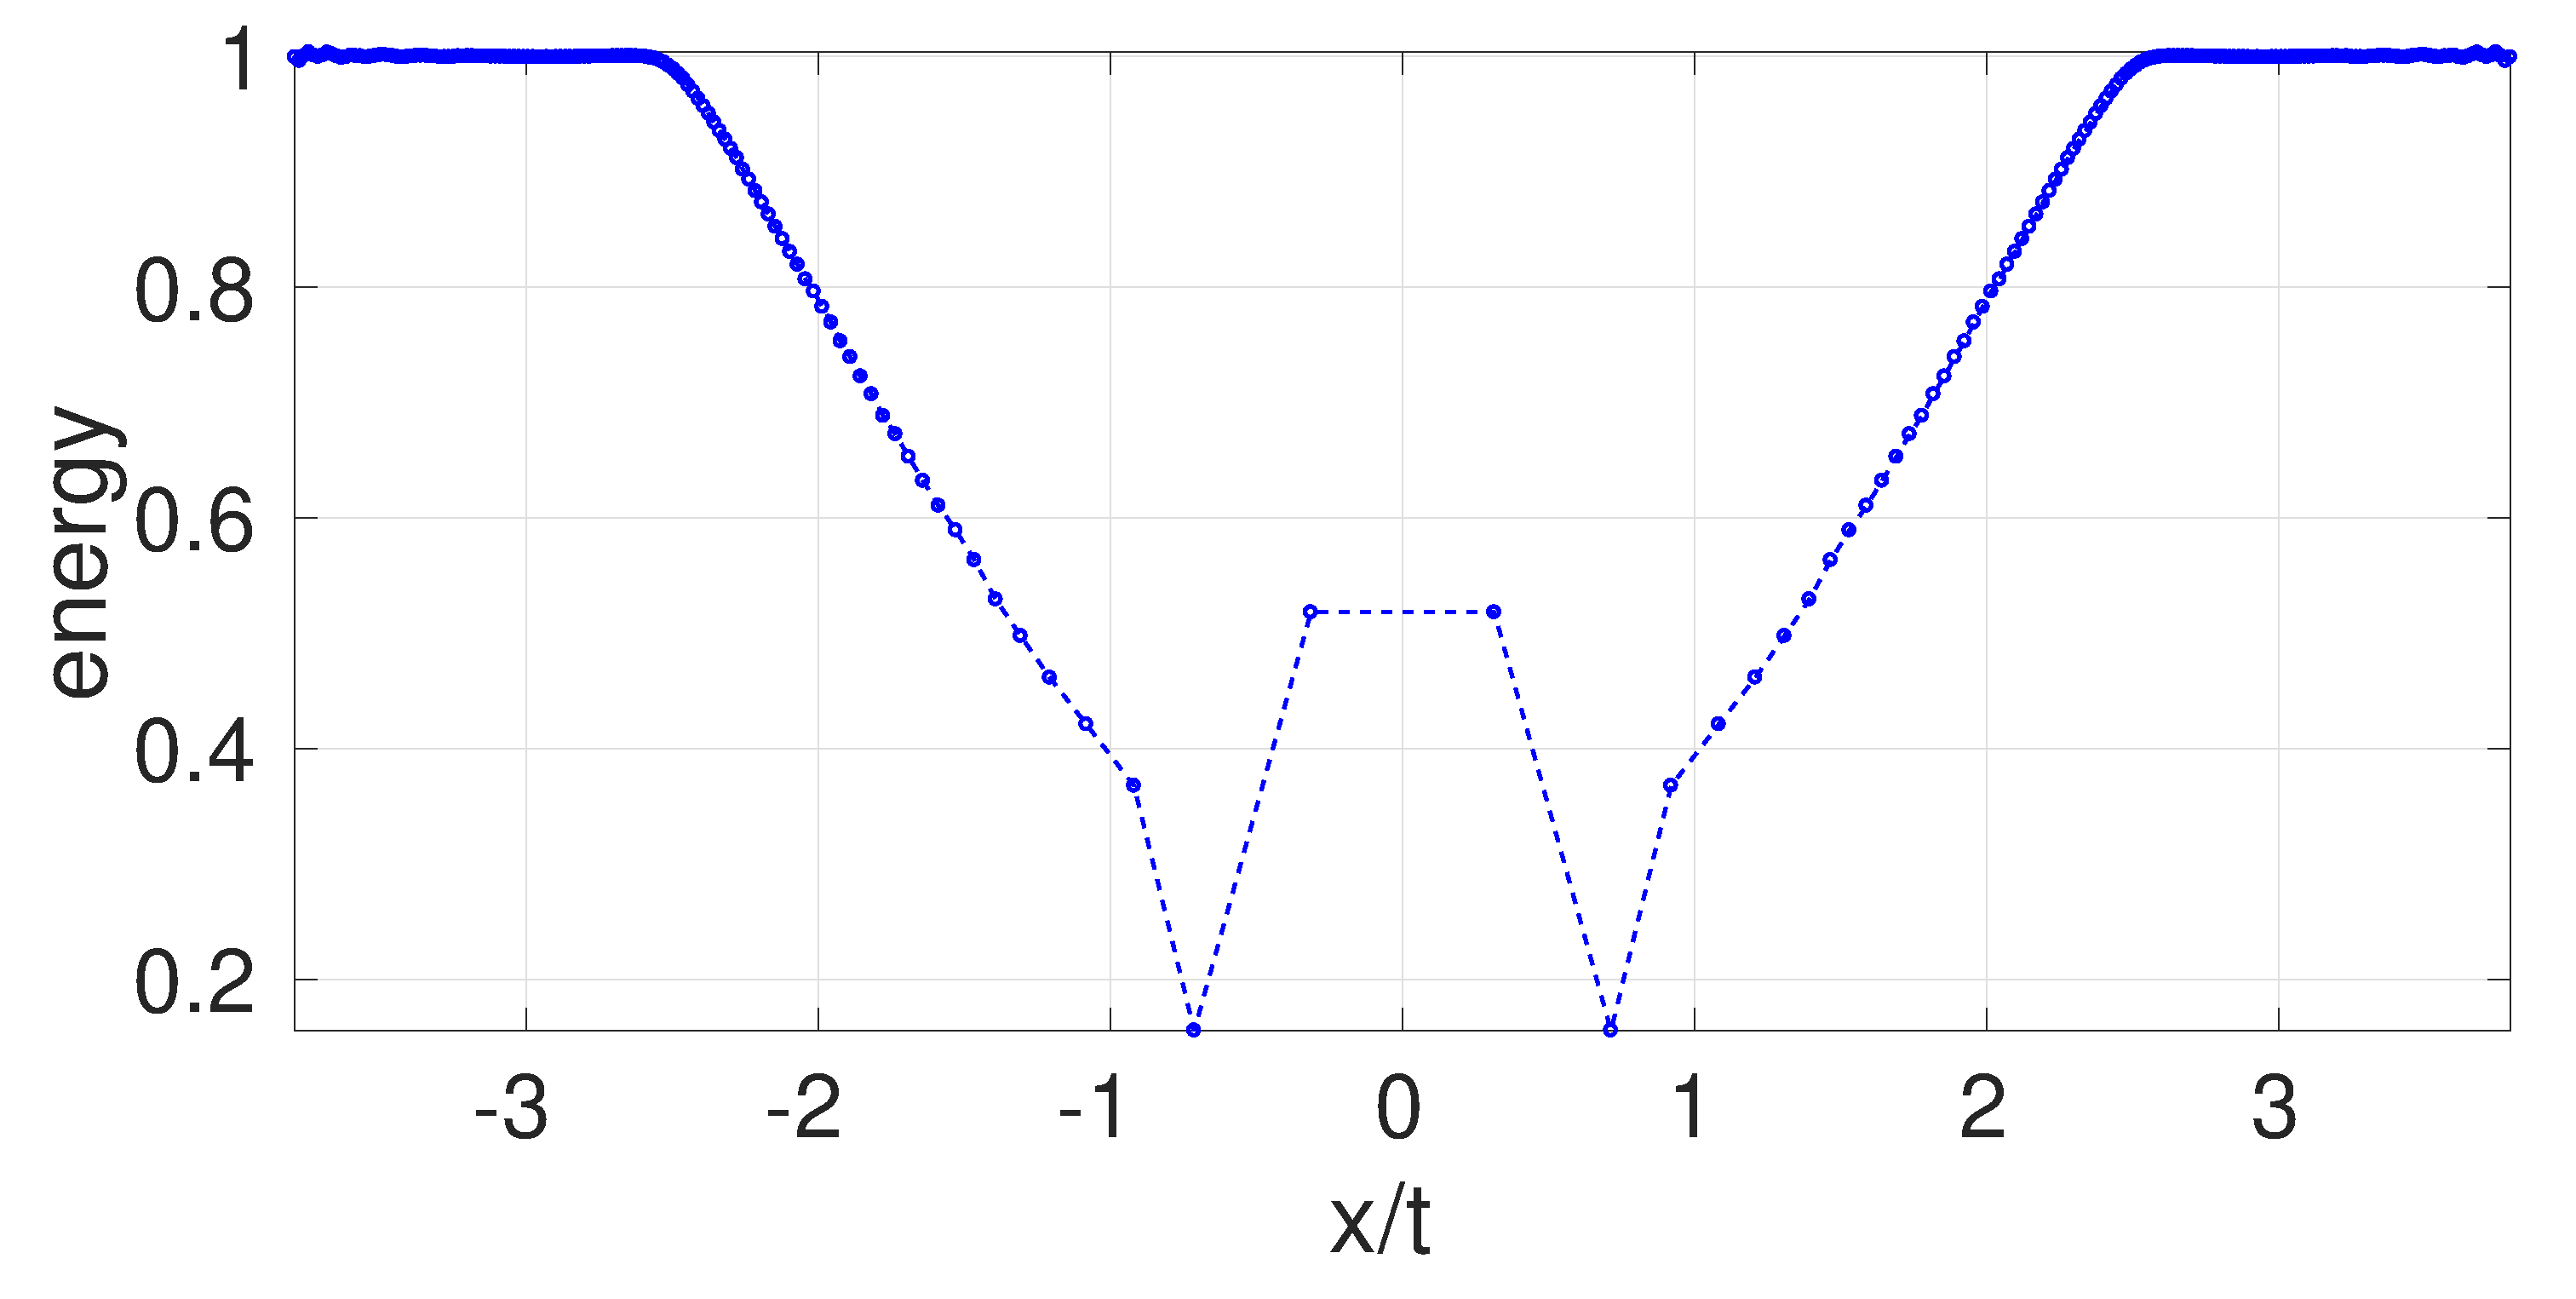
\includegraphics[width=0.99 \textwidth]{./Figures/Sjogreen/Sjogreen-RCM-e-Adpt1}
    \end{minipage}%
    \begin{minipage}{.245 \textwidth}
        \centering
        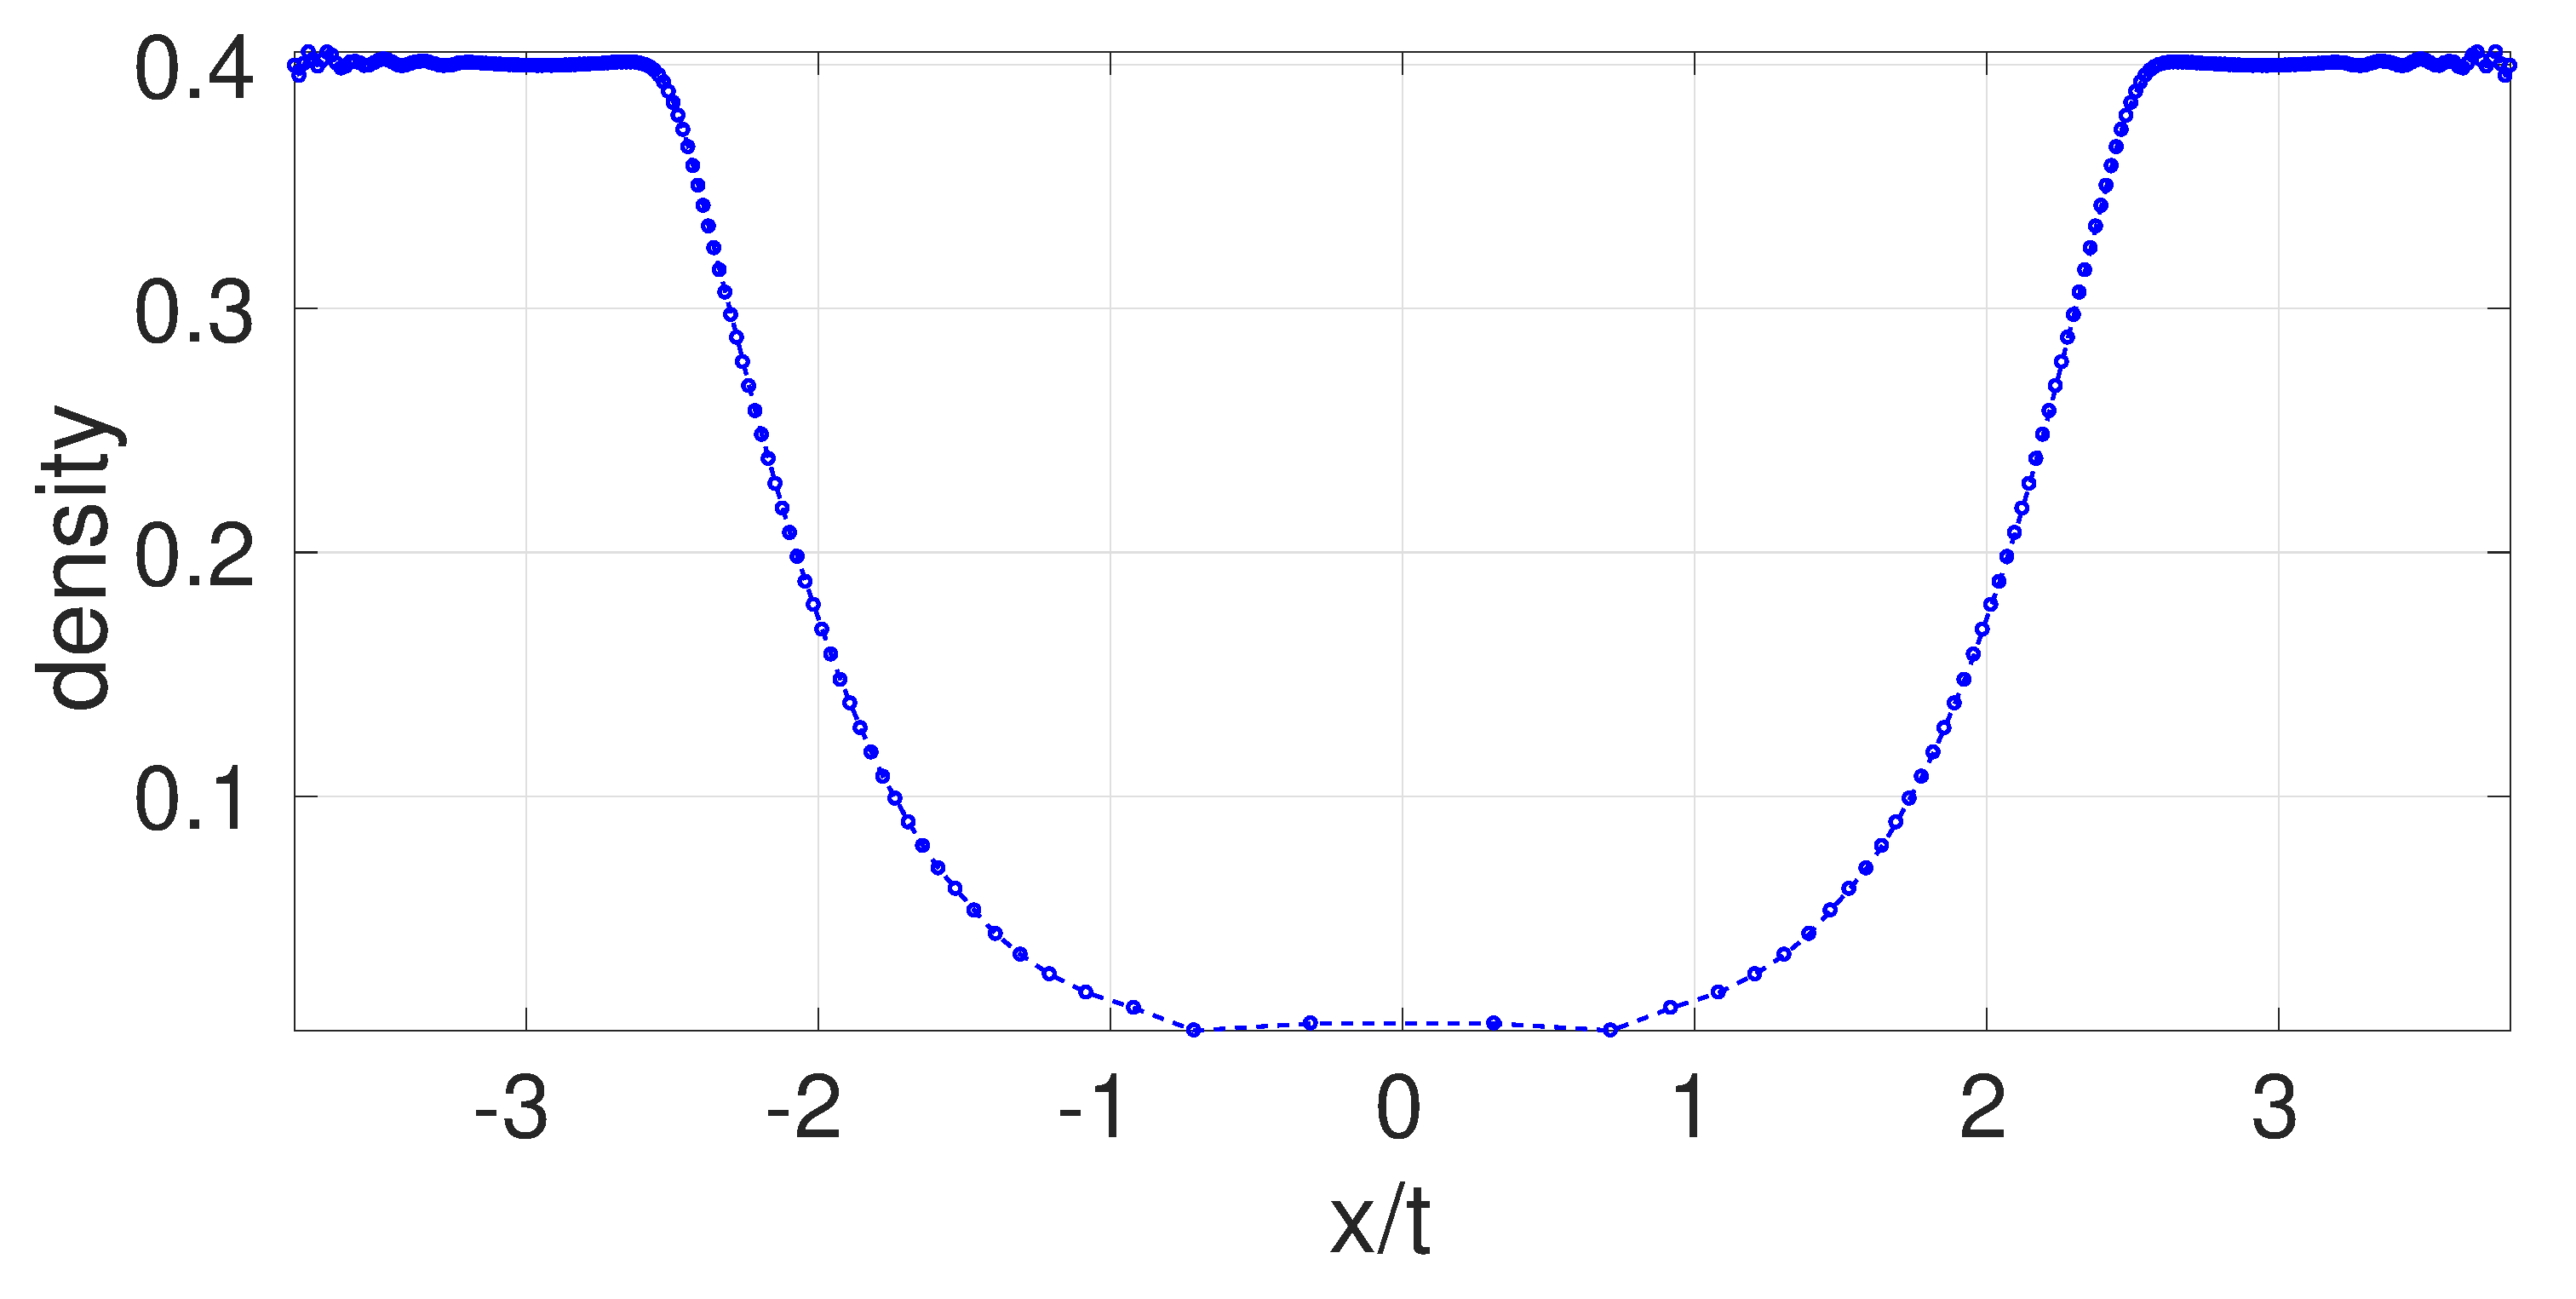
\includegraphics[width=0.99 \textwidth]{./Figures/Sjogreen/Sjogreen-RCM-p-Adpt1}
    \end{minipage}% 
    \caption{Results for test 5.}
    \label{fig:RCM-Sjogreen}
\end{figure}
\begin{figure}[H]
    \centering
    \begin{minipage}{.245\textwidth}
        \centering
        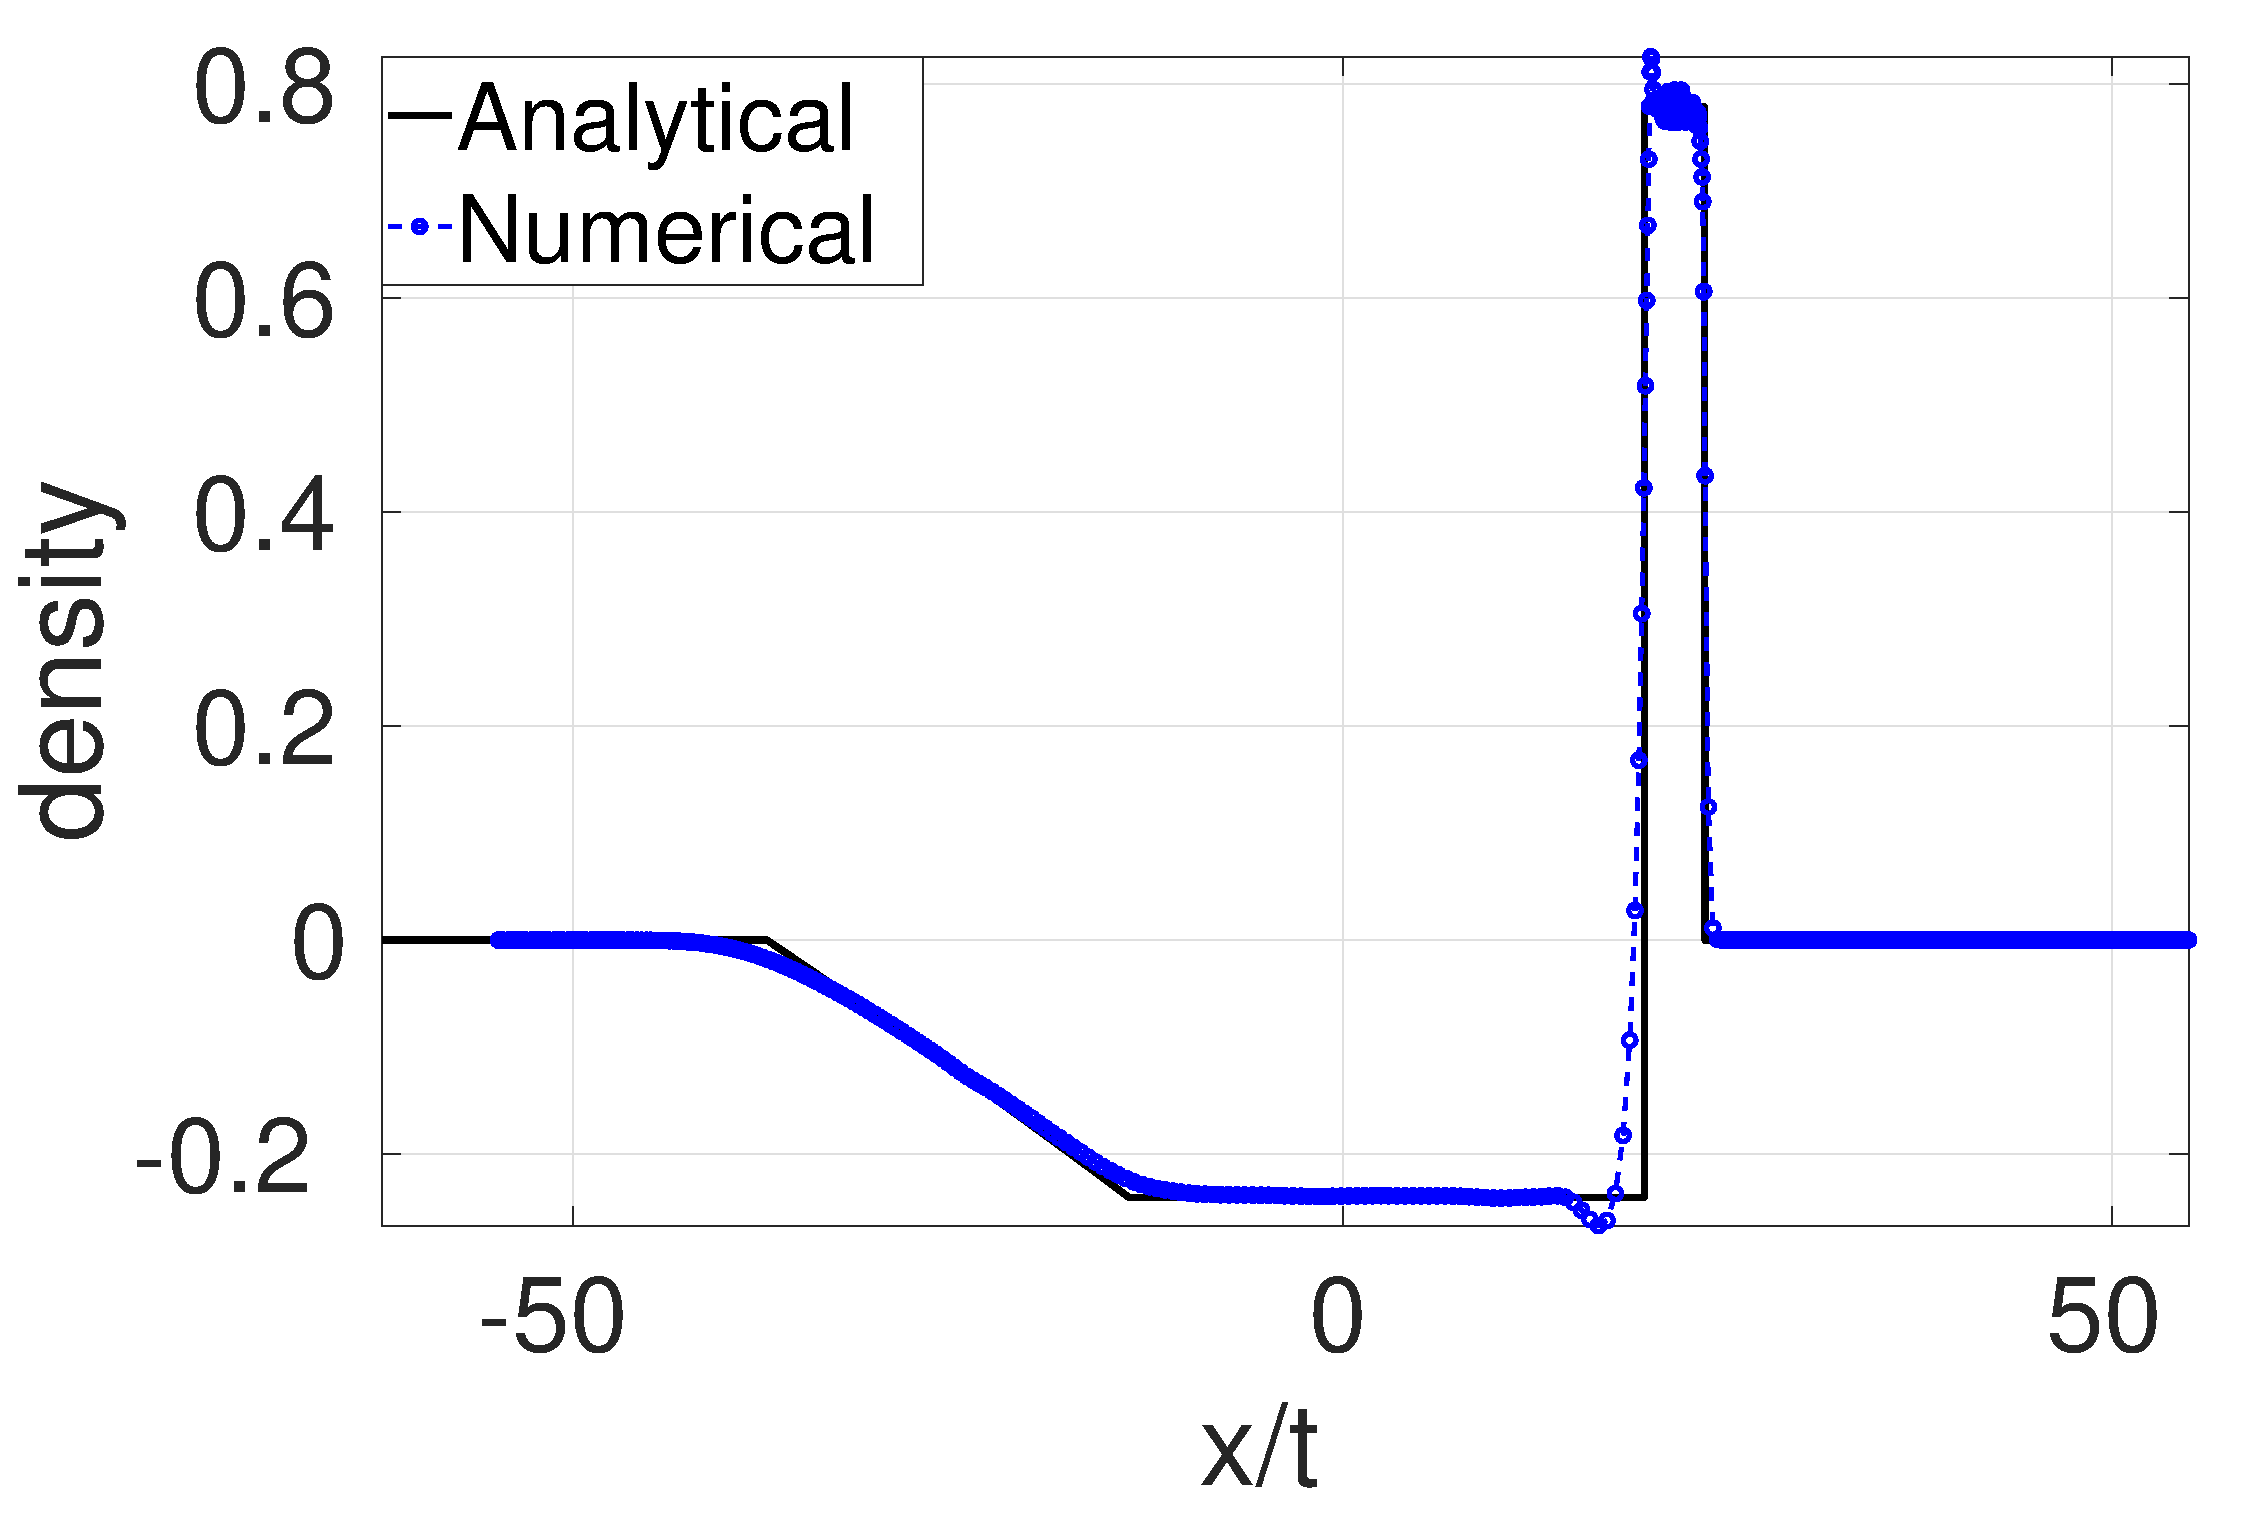
\includegraphics[width=0.99 \textwidth]{./Figures/strong-blast/StrBlst-RCM-rho-Rp3}
    \end{minipage}%
    \begin{minipage}{.245 \textwidth}
        \centering
        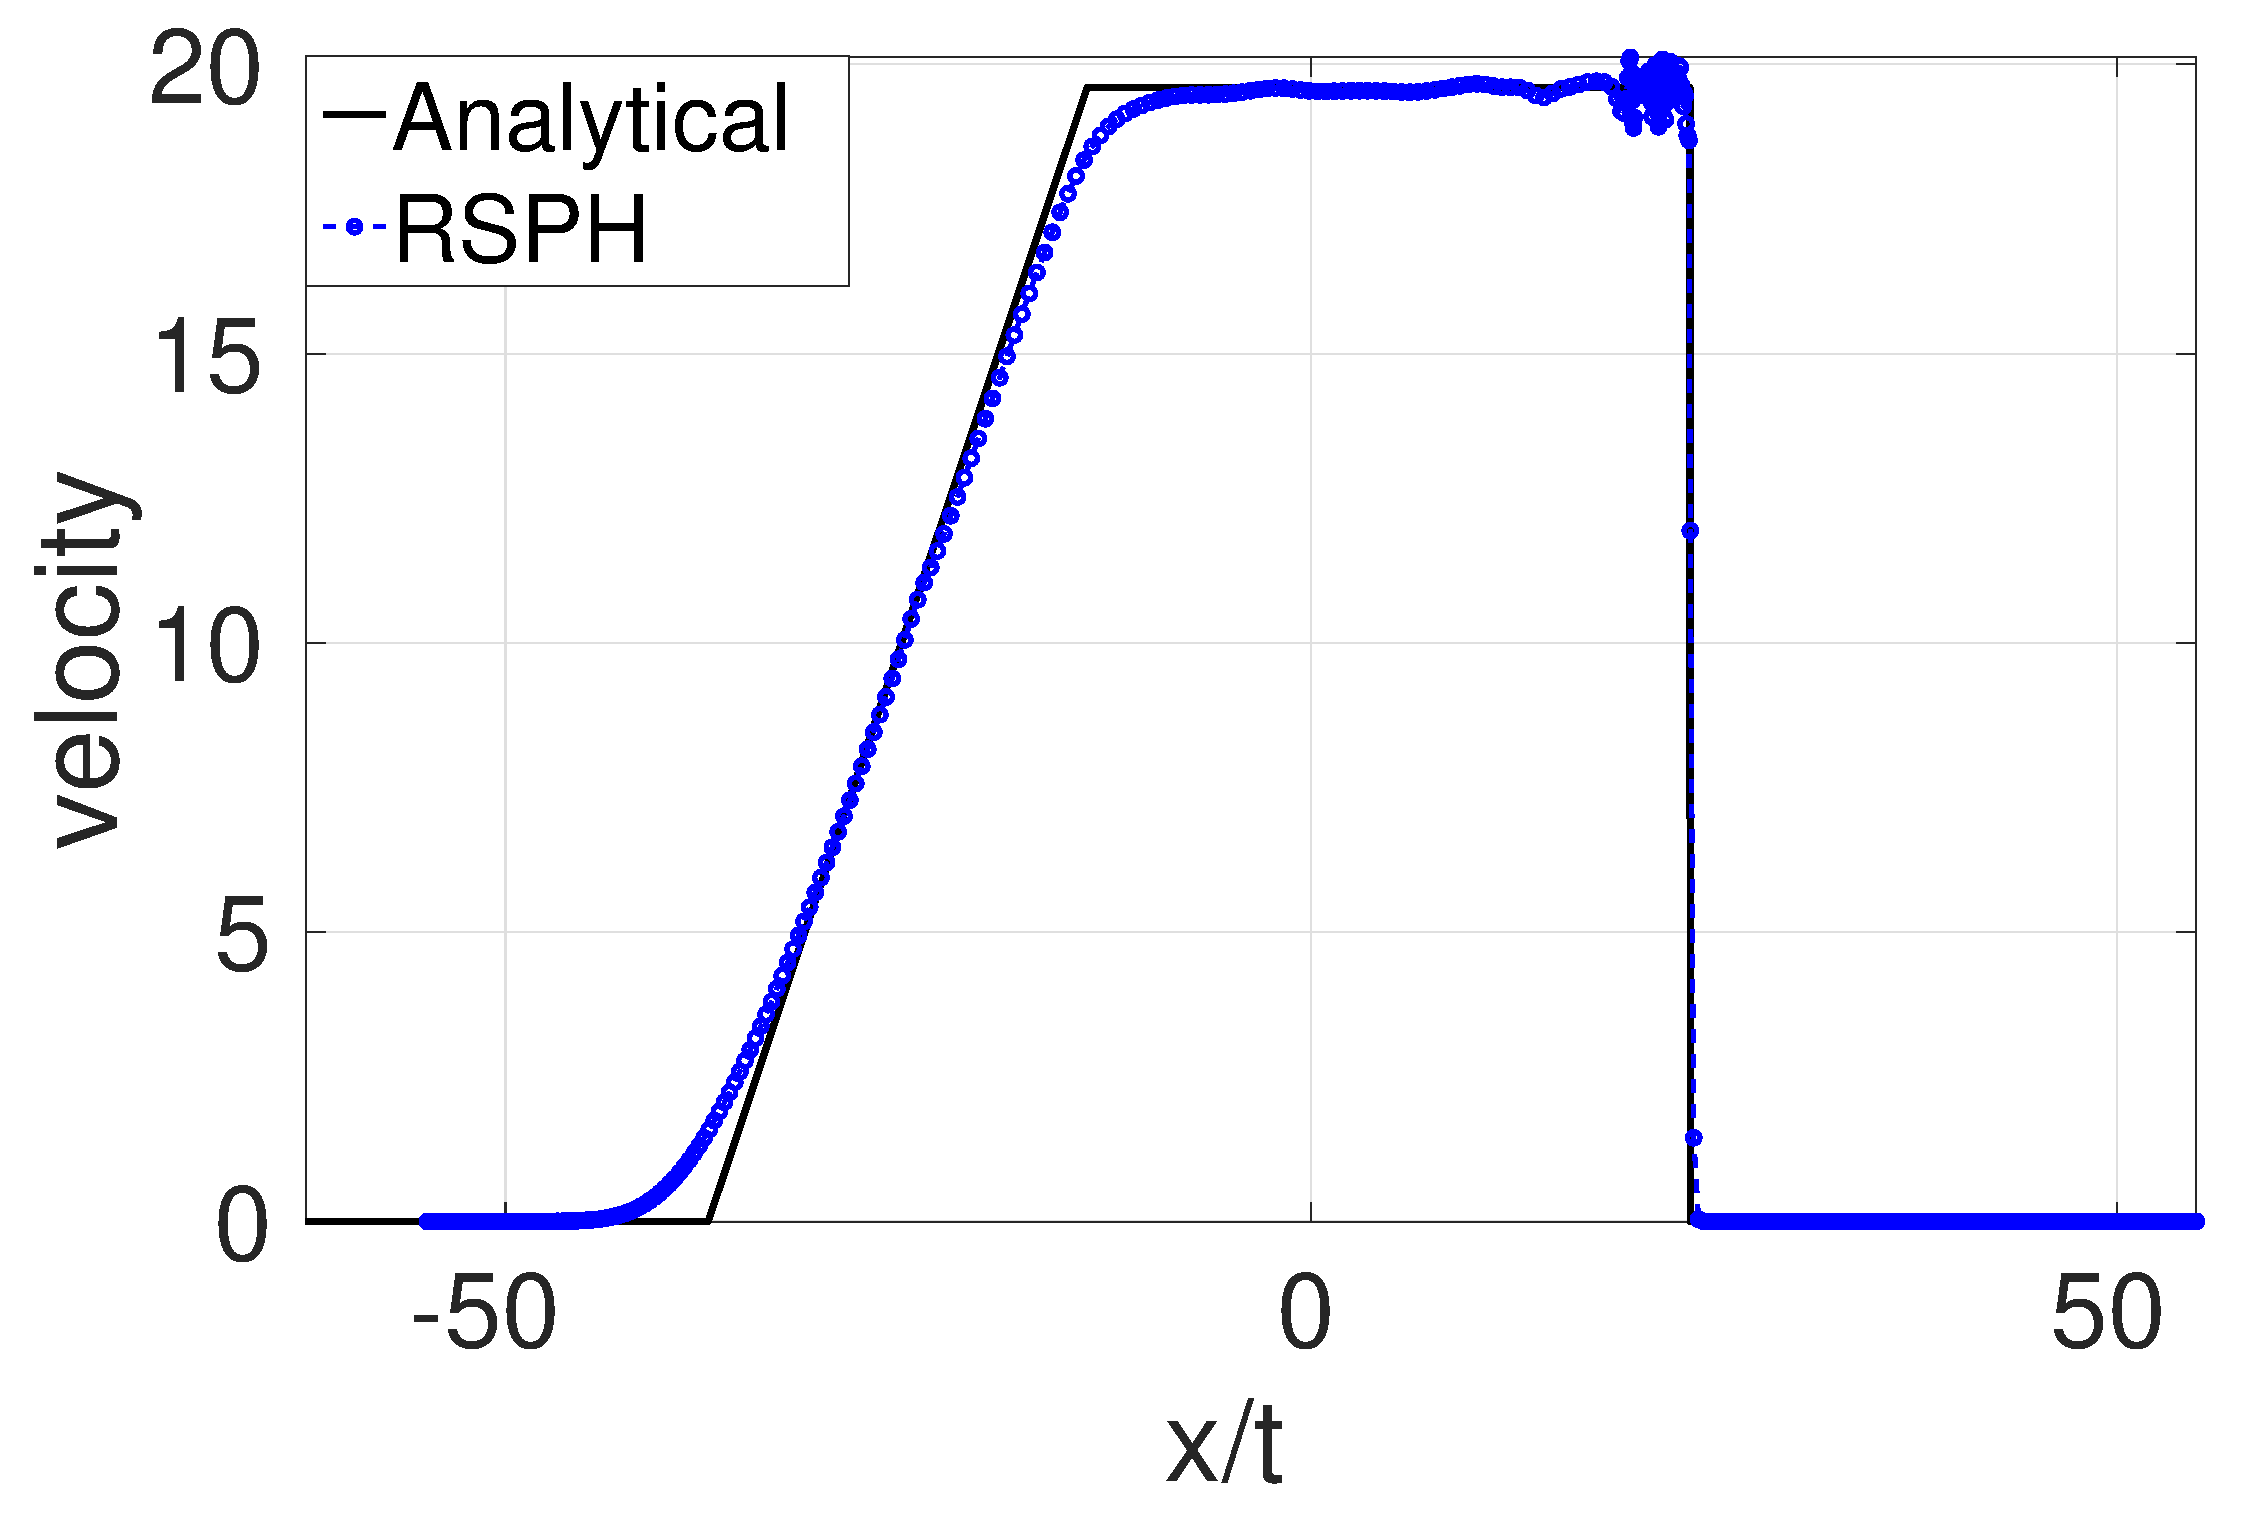
\includegraphics[width=0.99 \textwidth]{./Figures/strong-blast/StrBlst-RCM-v-Rp3}
    \end{minipage}%
    \begin{minipage}{.245\textwidth}
        \centering
        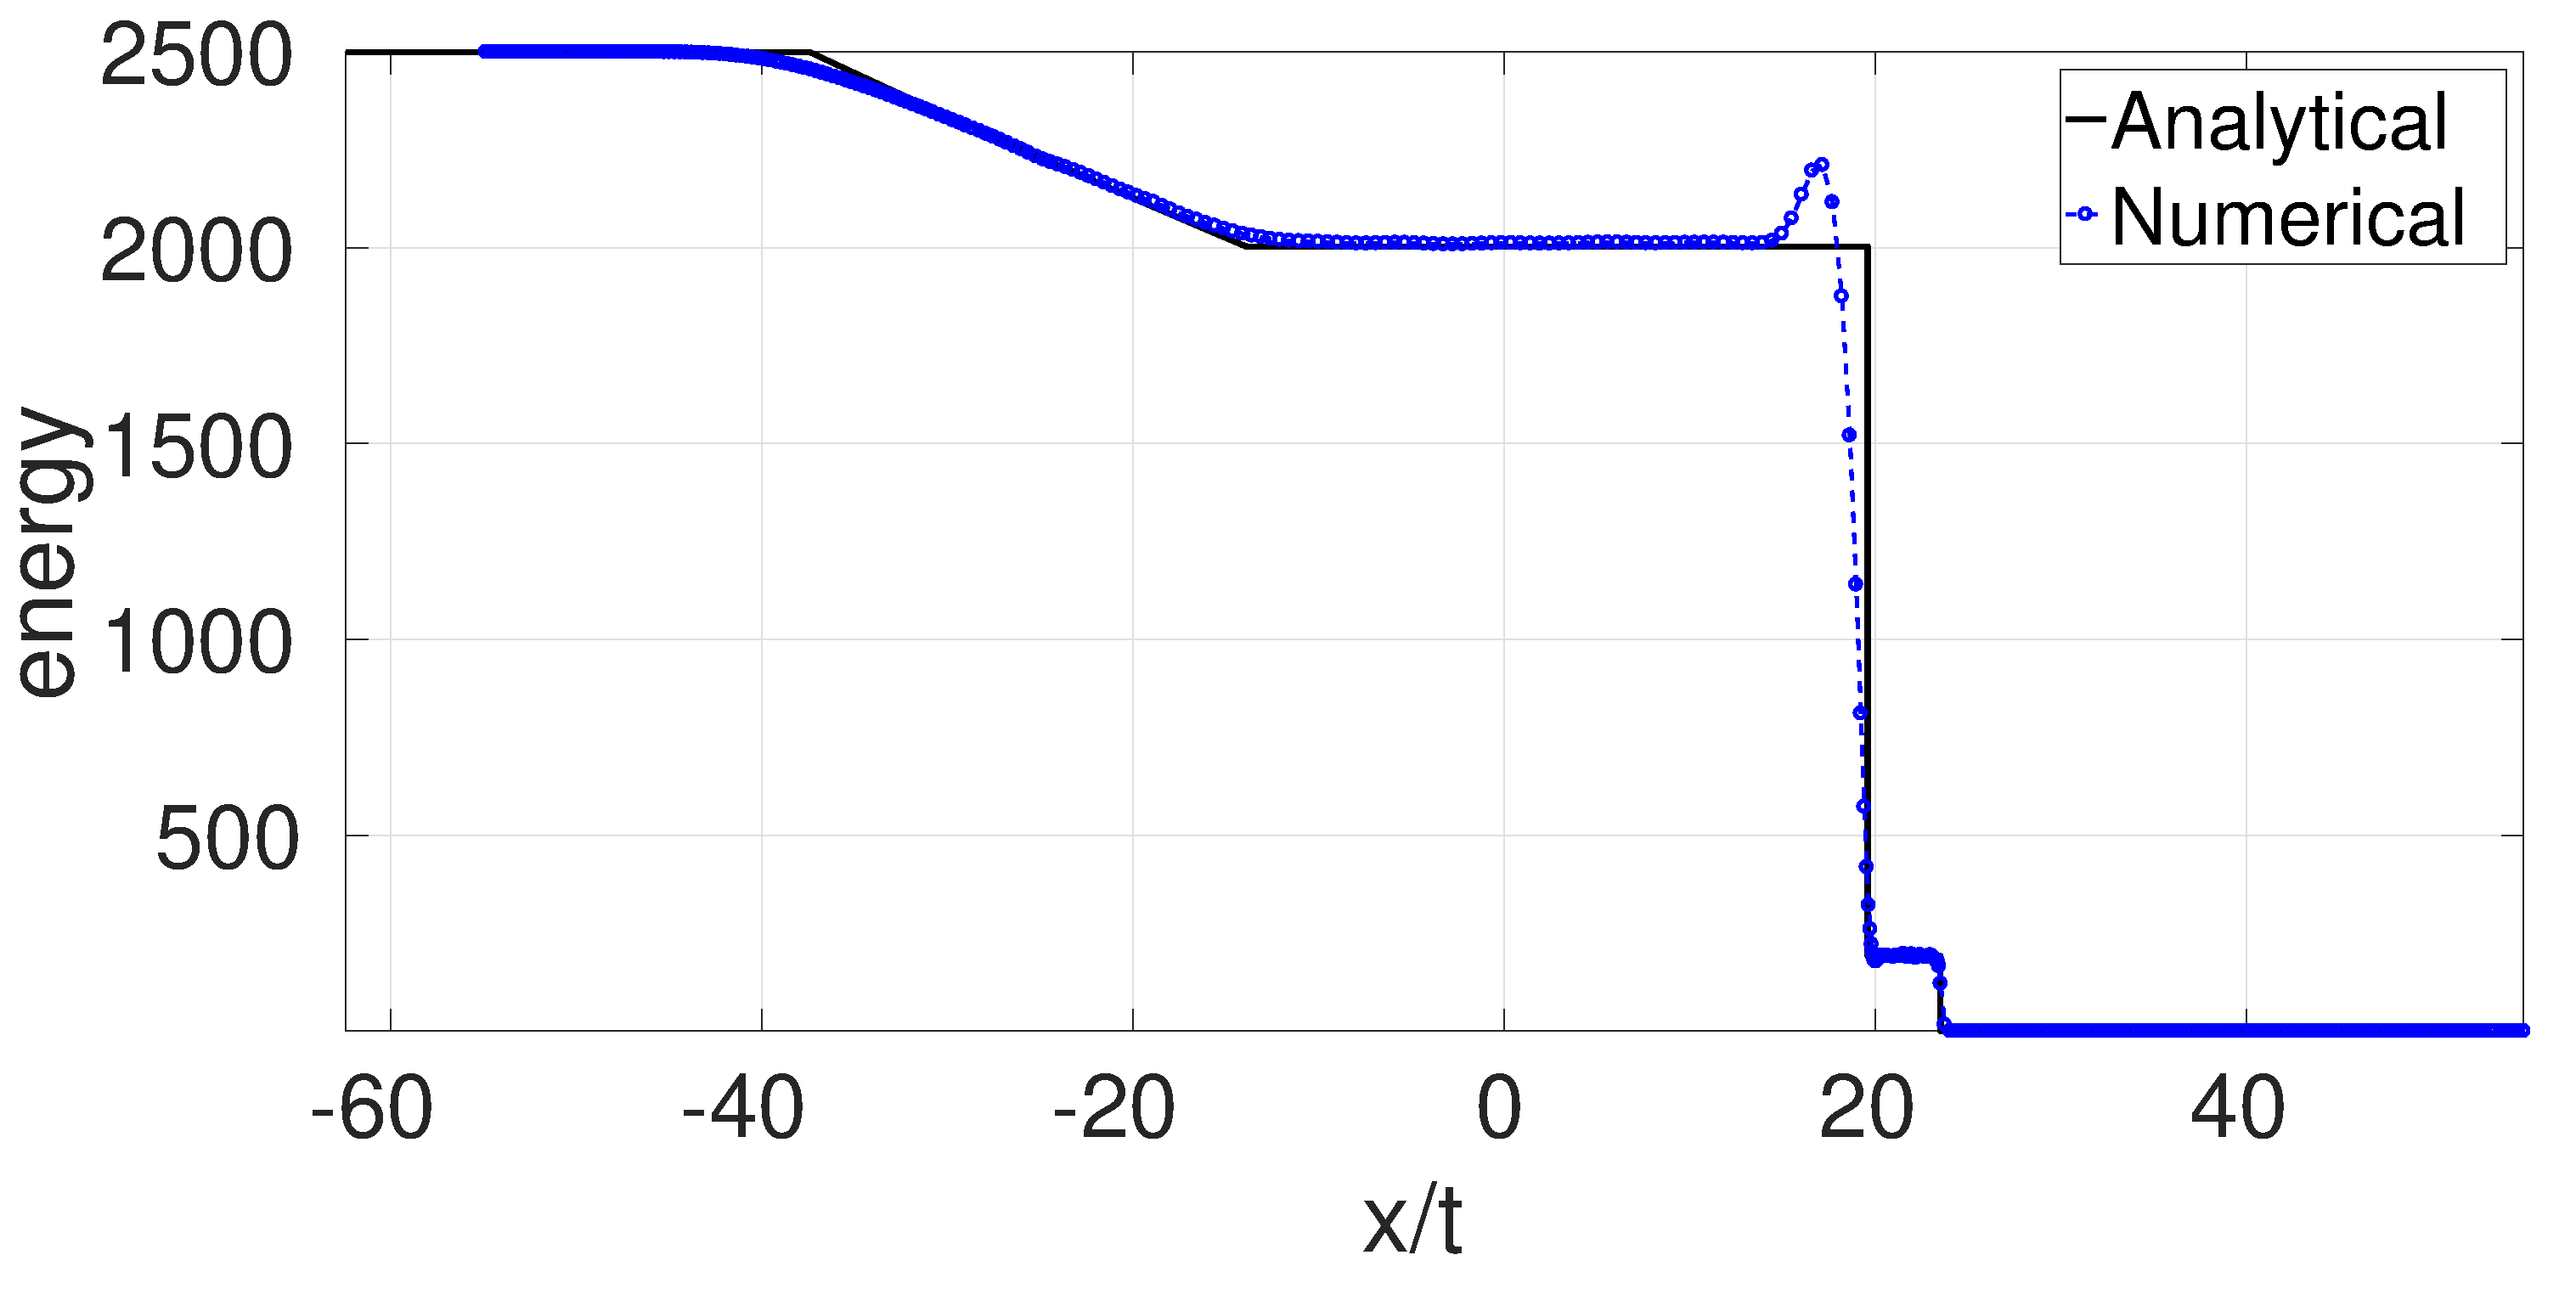
\includegraphics[width=0.99 \textwidth]{./Figures/strong-blast/StrBlst-RCM-e-Rp3}
    \end{minipage}%
    \begin{minipage}{.245 \textwidth}
        \centering
        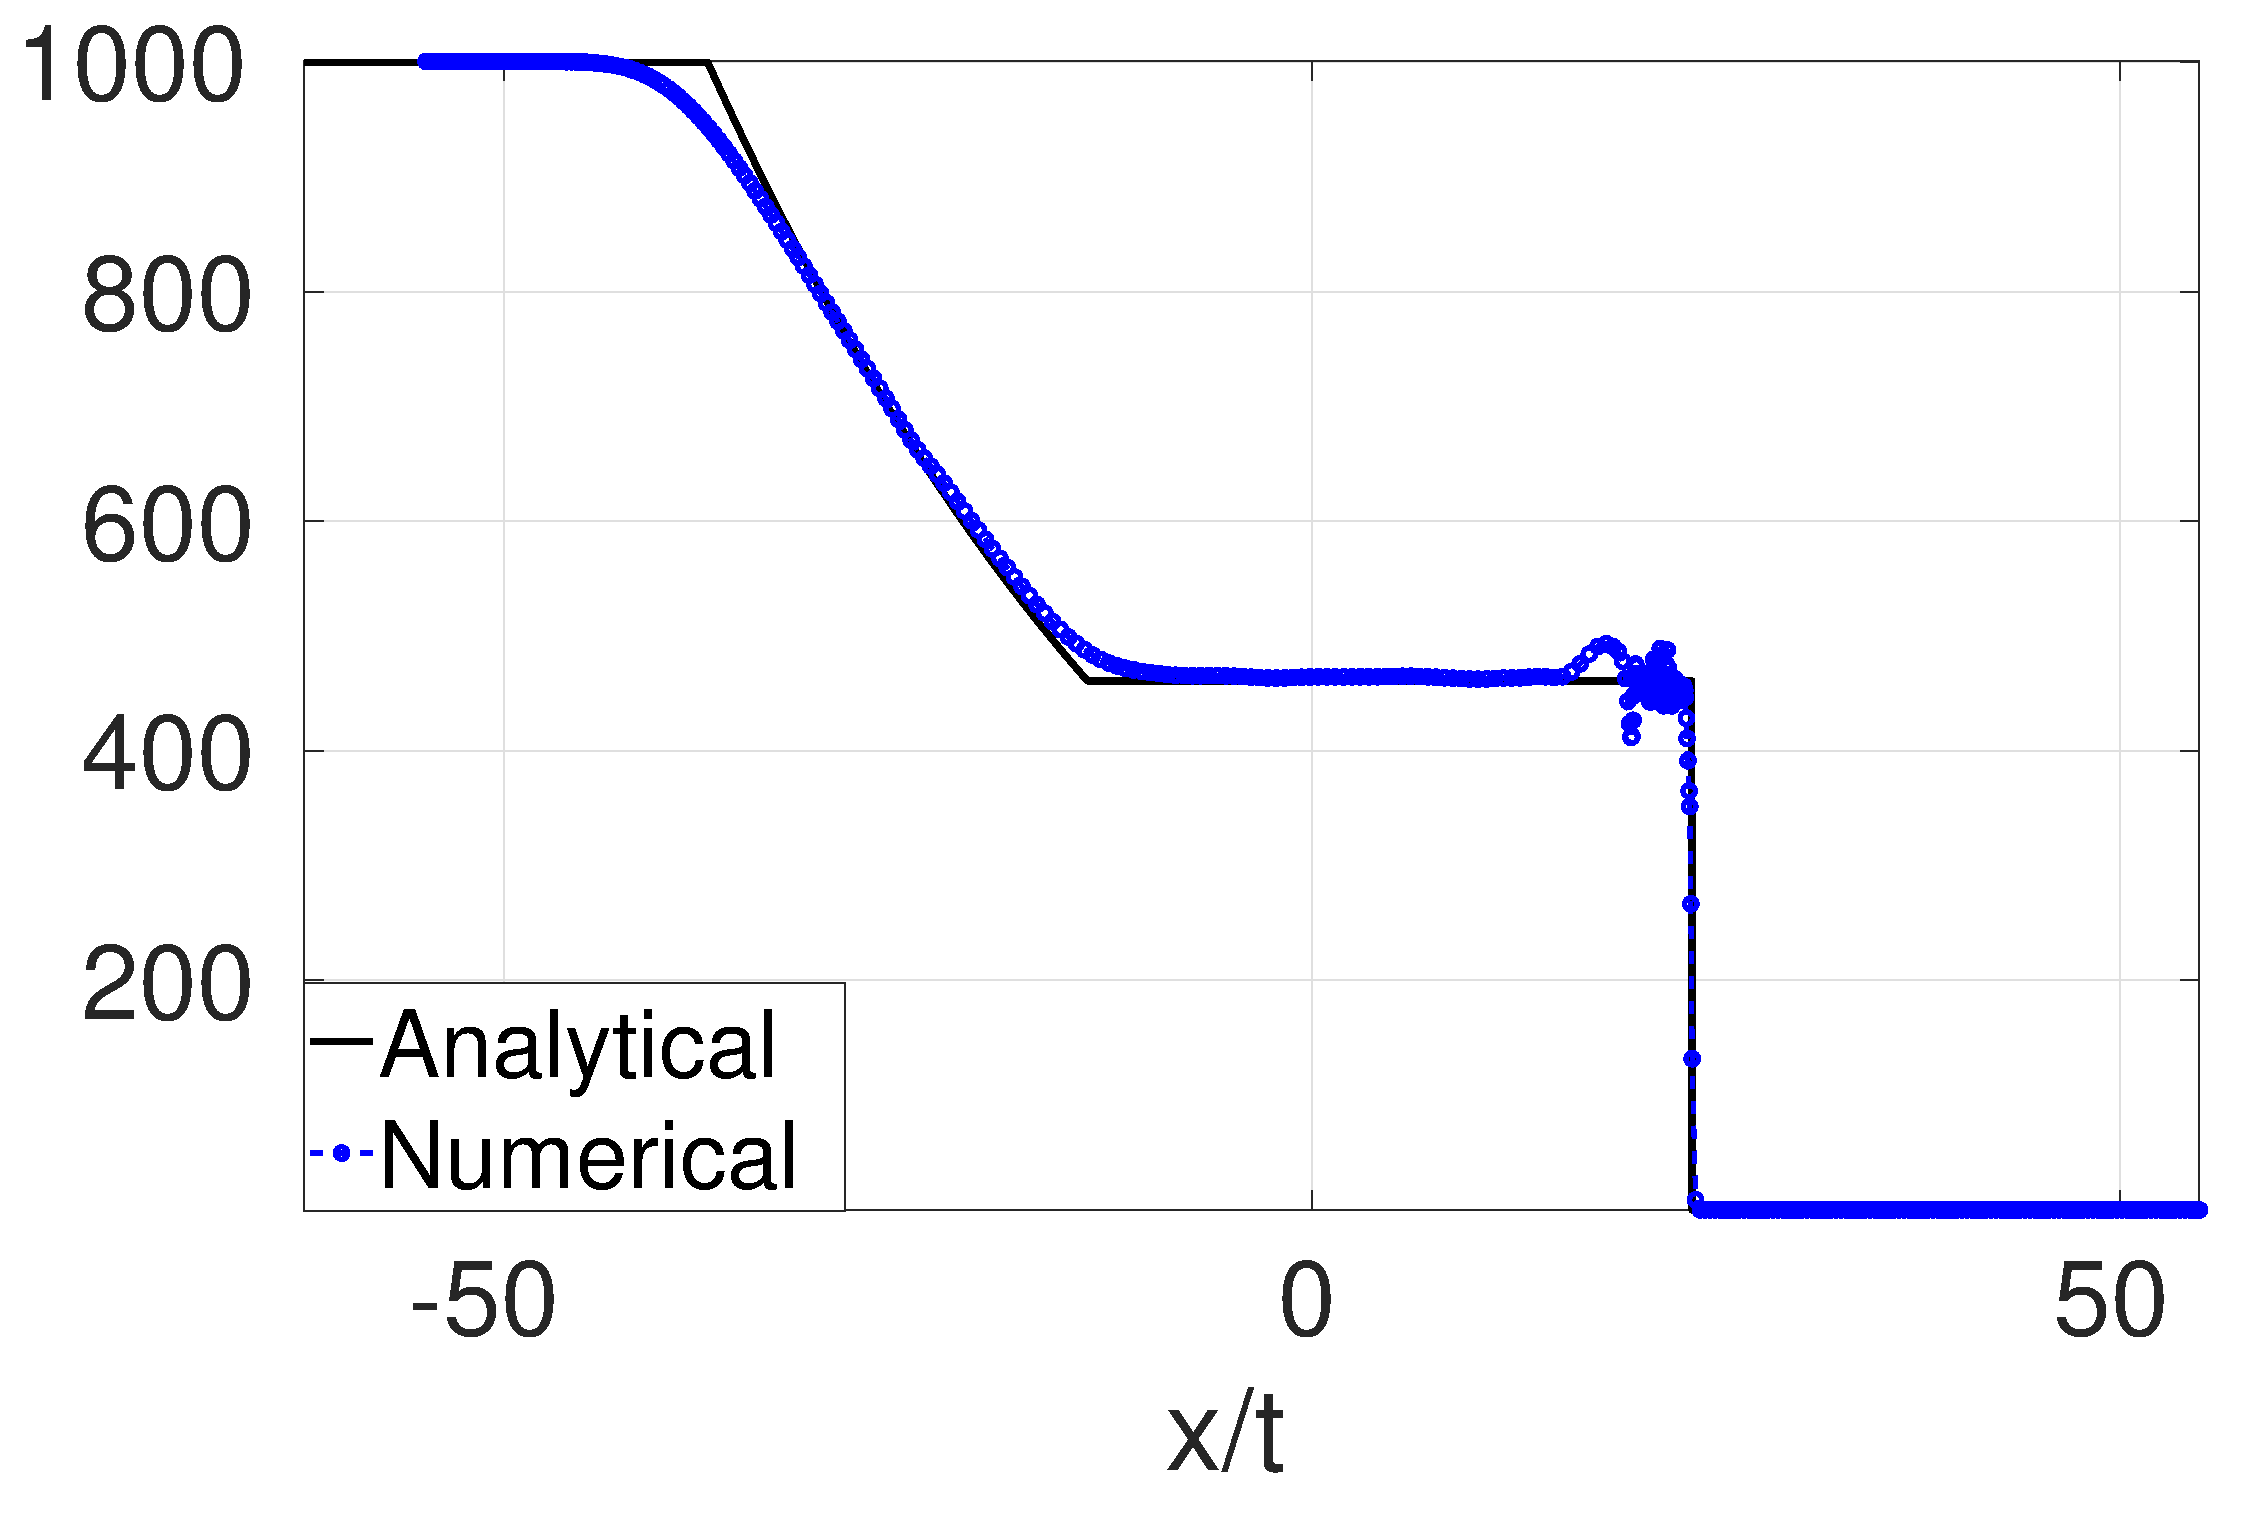
\includegraphics[width=0.99 \textwidth]{./Figures/strong-blast/StrBlst-RCM-p-Rp3}
    \end{minipage}% 
    \caption{Results for test 6.}
    \label{fig:RCM-strong-blast}
\end{figure}

\subsection{Simulation of 3D inject flow}

\section{Conclusion}
This new method enables shock capturing with lower dissipation. One potential application of the method is high speed mixing flow process, for example, supersonic combustion.
By overcoming a fundamental shortcoming of RCM and inheriting attractive feature of RCM, RSPH provide a powerful numerical method for solving combustion problems of in muti-dimensional space.

One limitation of RSPH is that for very strong shocks, simulation becomes unstable. In addition, numerical perturbation caused by non-uniform distribution of smoothing length in space can not be suppressed completely due to smaller dissipation introduced by RSPH in the area away from shocks.

\section*{References}
\bibliography{../Reference}
\end{document}
